Η έρευνα που παρουσιάζεται στο παρόν κεφάλαιο αντλεί τις πηγές της από τις
αιτίες περαιτέρω έρευνας του προηγούμενου κεφαλαίου, όπως αυτές διατυπώθηκαν
στην τελευταία του ενότητα. Στο παρόν κεφάλαιο επιζητούμε το σχεδιασμό και
την ανάπτυξη μεθόδου ευθυγράμμισης πραγματικών με εικονικές σαρώσεις η οποία
λειτουργεί (α) χωρίς τον υπολογισμό αντιστοιχίσεων ανάμεσα στις ακτίνες των
εισόδων της, (β) με ``μικρό" σύνολο ρυθμιζόμενων παραμέτρων, και (γ) με
επίδοση ως προς το σφάλμα στάσης τουλάχιστον ισάξια με την καλύτερη μέθοδο
ευθυγράμμισης μέσω αντιστοιχιών.

Ερευνώντας τη σχετική βιβλιογραφία ανακαλύψαμε την παντελή έλλειψη μεθόδων που
ικανοποιούν ταυτόχρονα τις παραπάνω απαιτήσεις, τις οποίες θεωρήσαμε ως
κρίσιμης σημασίας για τον στόχο της εκτίμησης της στάσης ενός οχήματος του
πεδίου εφαρμογής \ref{scope}. Για αυτόν τον λόγο επεκτείναμε την έρευνά μας σε
κλάδους διαφορετικούς από αυτόν της ρομποτικής, ώστε, σκεπτόμενοι και δρώντας
ως μηχανικοί, να μεταφράσουμε μεθόδους της ευρύτερης βιβλιογραφίας στα
συμφραζόμενα του προβλήματός μας, και να τις μεταγγίσουμε σε συστήματα που το
επιλύουν.

Σε αυτό το κεφάλαιο παρουσιάζουμε την προσαρμογή μίας μεθόδου από τον κλάδο της
υπολογιστικής όρασης για την επίλυση του προβλήματος της εύρεσης της στάσης
ενός ρομπότ στο δισδιάστατο επίπεδο. Πιο συγκεκριμένα θα ασχοληθούμε με την
επίλυση του προβλήματος βάσει \textit{καθολικής} αβεβαιότητος. Ο λόγος για τον
οποίο δεν συνεχίζουμε σε αυτό το σημείο την επίλυση του προβλήματος βάσει
πεπερασμένης αβεβαιότητος (όπως στο προηγούμενο κεφαλαίο) είναι η επιθυμία
δοκιμής της υπόθεσης \ref{hypothesis:02_03:01} \textit{επί της αρχής}:

\begin{customhypothesis}{Υ4}
\label{hypothesis:02_03:01}
  Υπάρχει μέθοδος ευθυγράμμισης πραγματικών με εικονικές
  σαρώσεις που δεν χρησιμοποιεί αντιστοιχίσεις, η οποία εμφανίζει ισάξια
  επίδοση με την καλύτερη μέθοδο ευθυγράμμισης πραγματικών με εικονικές
  σαρώσεις που χρησιμοποιεί τον υπολογισμό αντιστοιχίσεων για την επίλυση του
  προβλήματος ευθυγράμμισης.
\end{customhypothesis}

Αυτό σημαίνει ότι, σε αυτό το προκαταρκτικό στάδιο, ο χρόνος εκτέλεσης της
λύσης δεν αποτελεί κριτήριο αξιολόγησης---κάτι απαιτητέο στο πρόβλημα βάσει
πεπερασμένης αβεβαιότητος, δεδομένου ότι η επίλυση του πρέπει να γίνεται σε
πραγματικό χρόνο. Για αυτόν το λόγο εκμεταλλευόμαστε την παρατήρηση
\ref{remark:01_01_02_02:02} και προτείνουμε μία λύση στο πρόβλημα εντοπισμού
της στάσης ενός ρομπότ κινητής βάσης του πεδίου εφαρμογής \ref{scope} μέσω
ευθυγράμμισης πραγματικών με εικονικές σαρώσεις, η οποία ικανοποιεί τις
απαιτήσεις της πρώτης παραγράφου.

Κατά τη διάρκεια προκαταρκτικής έρευνας επί των ικανοτήτων της μεθόδου που
παρουσιάζεται σε αυτό το κεφάλαιο καταλήξαμε στο συμπέρασμα ότι:

\begin{claim}
\label{claim:02_03:01}
  Μία ικανή συνθήκη για την αφαίρεση του μηχανισμού υπολογισμού αντιστοιχίσεων
  είναι η αντικατάστασή του από αναλυτικές λύσεις του προβλήματος σε κλειστή
  μορφή.  Εκτιμούμε ότι μία αναγκαία συνθήκη για την ανάπτυξή αυτών των λύσεων
  είναι η περιοδικότητα των σαρώσεων, δηλαδή η πανοραμικότητα του γωνιακού
  εύρους των πραγματικών και εικονικών σαρώσεων.
\end{claim}

Αποτελεί ανοιχτό ερώτημα εάν αυτή η συνθήκη είναι αναγκαία ή απλά ικανή.

%%%%%%%%%%%%%%%%%%%%%%%%%%%%%%%%%%%%%%%%%%%%%%%%%%%%%%%%%%%%%%%%%%%%%%%%%%%%%%%%
\section{Στόχοι του κεφαλαίου και δομή}
  \label{section:02_03_01}
  Έστω $\theta = \hat{\theta} + \phi_0$, όπου $\phi_0$ είναι το αρχικό σφάλμα
εκτίμησης. Τότε η εξίσωση (\ref{eq:x1_for_proof}):
\begin{align}
  -\mathcal{F}_1\{\mathcal{S}_V\} &= -e^{-i(\theta-\hat{\theta})} \mathcal{F}_1\{\mathcal{S}_R\}- N_s e^{i\hat{\theta}}(\delta_x - i\cdot \delta_y) \nonumber\\
  \mathcal{F}_1\{\mathcal{S}_V\} &= e^{-i\phi_0} \mathcal{F}_1\{\mathcal{S}_R\}+ N_s e^{i\hat{\theta}}(\delta_x - i\cdot \delta_y) \nonumber
\end{align}

Έστω $\delta = \delta_x - i \cdot \delta_y$. Τότε
\begin{align}
  e^{i\phi_0} &= \dfrac{\mathcal{F}_1\{\mathcal{S}_R\}}{\mathcal{F}_1\{\mathcal{S}_V\} - N_s e^{i\hat{\theta}}\delta}  \label{eq:appendix:02:04:01_01}
\end{align}

Έστω $B = \mathcal{F}_1\{\mathcal{S}_V\} - N_s e^{i\hat{\theta}}\delta$ ο
παρονομαστής της εξίσωσης (\ref{eq:appendix:02:04:01_01}). Τότε
\begin{align}
  B &= |\mathcal{F}_1\{\mathcal{S}_V\}| e^{i\angle \mathcal{F}_1\{\mathcal{S}_V\}} - N_s e^{i\hat{\theta}}|\delta| e^{i \angle \delta} \nonumber \\
    &= [ |\mathcal{F}_1\{\mathcal{S}_V\}| \cos(\angle \mathcal{F}_1\{\mathcal{S}_V\}) - N_s |\delta| \cos(\hat{\theta} + \angle\delta) ] \nonumber \\
    &+ i\cdot [ |\mathcal{F}_1\{\mathcal{S}_V\}| \sin(\angle \mathcal{F}_1\{\mathcal{S}_V\}) - N_s |\delta| \sin(\hat{\theta} + \angle\delta) ] \nonumber \\
    &= |B| e^{i \angle B}
\end{align}
όπου
\begin{align}
  |B| = |\mathcal{F}_1\{\mathcal{S}_V\}|^2 + N_s^2|\delta|^2 -2 |\mathcal{F}_1\{\mathcal{S}_V\}| N_s |\delta| \cos(\angle \mathcal{F}_1\{\mathcal{S}_V\}-\hat{\theta} - \angle\delta) \nonumber
\end{align}
και
\begin{align}
  \angle B = \tan^{-1} \dfrac{ |\mathcal{F}_1\{\mathcal{S}_V\}| \sin(\angle \mathcal{F}_1\{\mathcal{S}_V\}) - N_s |\delta| \sin(\hat{\theta} + \angle\delta)}{|\mathcal{F}_1\{\mathcal{S}_V\}| \cos(\angle \mathcal{F}_1\{\mathcal{S}_V\}) - N_s |\delta| \cos(\hat{\theta} + \angle\delta)} \label{eq:appendix:02:04:01_02}
\end{align}

Τότε η εξίσωση (\ref{eq:appendix:02:04:01_01}) γίνεται
\begin{align}
  e^{i\phi_0} &= \dfrac{\mathcal{F}_1\{\mathcal{S}_R\}}{B} \nonumber \\
  e^{i\phi_0} &= \dfrac{|\mathcal{F}_1\{\mathcal{S}_R\}| e^{i \angle \mathcal{F}_1\{\mathcal{S}_R\}}}{|B| e^{i \angle B}} \nonumber \\
  e^{i\phi_0} &= \dfrac{|\mathcal{F}_1\{\mathcal{S}_R\}|}{|B|}e^{i \angle \mathcal{F}_1\{\mathcal{S}_R\} - \angle B} \nonumber \\
       \phi_0 &= \angle \mathcal{F}_1\{\mathcal{S}_R\} - \angle B \label{eq:appendix:02:04:01_03}
\end{align}
Όμως, λόγω των εξισώσεων $\theta = \hat{\theta} + \phi_0$ και
(\ref{eq:update_t2}):
\begin{align}
  \theta &= \hat{\theta}^\prime + \phi \nonumber \\
  \theta &= \hat{\theta} + \angle \mathcal{F}_1\{\mathcal{S}_R\} - \angle\mathcal{F}_1\{\mathcal{S}_V\} + \phi \nonumber \\
  \phi_0 &= \angle \mathcal{F}_1\{\mathcal{S}_R\} - \angle\mathcal{F}_1\{\mathcal{S}_V\} + \phi \nonumber \\
  \angle \mathcal{F}_1\{\mathcal{S}_R\} - \angle B &\leftstackrel{(\ref{eq:appendix:02:04:01_03})}{=} \angle \mathcal{F}_1\{\mathcal{S}_R\} - \angle\mathcal{F}_1\{\mathcal{S}_V\} + \phi \nonumber \\
  - \angle B &= - \angle\mathcal{F}_1\{\mathcal{S}_V\} + \phi \nonumber \\
  \phi &= \angle\mathcal{F}_1\{\mathcal{S}_V\} - \angle B  \nonumber \\
  \phi &\leftstackrel{(\ref{eq:appendix:02:04:01_02})}{=} \angle\mathcal{F}_1\{\mathcal{S}_V\} - \tan^{-1} \dfrac{ |\mathcal{F}_1\{\mathcal{S}_V\}| \sin(\angle \mathcal{F}_1\{\mathcal{S}_V\}) - N_s |\delta| \sin(\hat{\theta} + \angle\delta)}{|\mathcal{F}_1\{\mathcal{S}_V\}| \cos(\angle \mathcal{F}_1\{\mathcal{S}_V\}) - N_s |\delta| \cos(\hat{\theta} + \angle\delta)} \nonumber \\
\end{align}
\qedsymbol


%%%%%%%%%%%%%%%%%%%%%%%%%%%%%%%%%%%%%%%%%%%%%%%%%%%%%%%%%%%%%%%%%%%%%%%%%%%%%%%%
\section{Σχετική βιβλιογραφία}
  \label{section:02_03_02}
  Έστω οι παραδοχές του προβλήματος \ref{prob:02_04}. Έστω επιπλέον ότι $\hat{\bm{l}} =
\bm{l}$, δηλαδή μόνο ο προσανατολισμός του αισθητήρα πρέπει να εκτιμηθεί. Τότε
ας υπολογιστεί η εικονική σάρωση $\mathcal{S}_V$ μέσω δεσμοβολής (raycasting)
από την εκτίμηση $\hat{\bm{p}}$ στον χάρτη $\bm{M}$. Η εκτίμηση της περιστροφής
της εικονικής σάρωσης $\mathcal{S}_V$ σε σχέση με την πραγματική σάρωση
$\mathcal{S}_R$ μπορεί να βρεθεί μέσω των μεθόδων που παρουσιάζονται στις
ενότητες \ref{subsection:02_04_02:01}, \ref{subsection:02_04_02:02}, και
\ref{subsection:02_04_02:03}. Το σφάλμα της εκτίμησης προσανατολισμού μπορεί να
μειωθεί περαιτέρω μέσω της μεθόδου που παρουσιάζεται στην ενότητα
\ref{subsection:02_04_02:06}.

Στα συμφραζόμενα του παρόντος κεφαλαίου, έστω $\mathcal{F}\{\mathcal{S}\}$ ο
διακριτός μετασχηματισμός Fourier του σήματος $\mathcal{S}$,
$\mathcal{F}^{-1}\{\mathcal{S}\}$ ο αντίστροφός του,
$\mathcal{F}_1\{\mathcal{S}\}$ ο πρώτος όρος του μετασχηματισμού (υποθέτοντας
αρίθμηση από το μηδέν), $\bm{c}^\ast$ ο συζυγής του μιγαδικού αριθμού $\bm{c}$,
$|\bm{c}|$ το μέτρο του, και $i$ η φανταστική μονάδα.

%%%%%%%%%%%%%%%%%%%%%%%%%%%%%%%%%%%%%%%%%%%%%%%%%%%%%%%%%%%%%%%%%%%%%%%%%%%%%%%%
\subsection{Η μέθοδος Fourier-Mellin σε μία διάσταση}
\label{subsection:02_04_02:01}

Έστω ότι ο χώρος δειγματοληπτείται επαρκώς πυκνά γωνιακά, τότε για
$k,\xi \in \mathbb{Z}_{\geq 0}$: $k,\xi \in [0, N_s-1]$:
\begin{align}
  \mathcal{S}_V[k] &\simeq \mathcal{S}_R[(k - \xi) \mod N_s] \Rightarrow \nonumber \\
  \mathcal{F}\{\mathcal{S}_V\}(u) &\simeq e^{-i 2\pi \xi u / N_s} \cdot \mathcal{F}\{\mathcal{S}_R\}(u) \nonumber
\end{align}
και, επομένως, αφού $2\pi \dfrac{\xi}{N_s} = \xi \dfrac{2\pi}{N_s} = \xi \gamma$,
όπου $\gamma$ είναι η διακριτική γωνία του αισθητήρα:
\begin{align}
  Q_{\mathcal{S}_V, \mathcal{S}_R}(u) & \triangleq \dfrac{\mathcal{F}\{\mathcal{S}_V\}^{\ast} \cdot \mathcal{F}\{\mathcal{S}_R\}}{|\mathcal{F}\{\mathcal{S}_V\}| \cdot |\mathcal{F}\{\mathcal{S}_R\}|} \nonumber \\
  &\simeq \dfrac{e^{-i \xi \gamma u} \cdot \mathcal{F}\{\mathcal{S}_R\}^\ast \cdot \mathcal{F}\{\mathcal{S}_R\}}{|e^{- i \xi \gamma u} \cdot \mathcal{F}\{\mathcal{S}_R\}^\ast | \cdot | \mathcal{F}\{\mathcal{S}_R\}|} \nonumber \\
  &= e^{-i \xi \gamma u} \cdot \dfrac{\mathcal{F}\{\mathcal{S}_R\}^\ast \cdot \mathcal{F}\{\mathcal{S}_R\}}{|\mathcal{F}\{\mathcal{S}_R\} | \cdot | \mathcal{F}\{\mathcal{S}_R\}|} \nonumber \\
  &= e^{-i \xi \gamma u}
  \label{eq:Q0}
\end{align}

Ο αντίστροφος διακριτός μετασχηματισμός Fourier του
$Q_{\mathcal{S}_V, \mathcal{S}_R}$ είναι μία Kronecker $\delta$-συνάρτηση
$q_{\mathcal{S}_V, \mathcal{S}_R} = \mathcal{F}^{-1}\{Q_{\mathcal{S}_V, \mathcal{S}_R}\}$
με κέντρο $\xi$:
\begin{align}
  \xi = \operatorname*{arg\,max}\limits_u \ q_{\mathcal{S}_V, \mathcal{S}_R}(u)
  \label{eq:02_04_02:xi}
\end{align}

Εάν η διαφορά του προσανατολισμού μεταξύ των στάσεων από τις οποίες ελήφθησαν
οι σαρώσεις $\mathcal{S}_R$ και $\mathcal{S}_V$ είναι
$\Delta\theta = \theta - \hat{\theta}$, τότε
$\Delta\theta = \xi\gamma + \phi$, όπου
$\mod(\Delta\theta, \gamma) = \phi \in [-\dfrac{\gamma}{2},+\dfrac{\gamma}{2}]$.
Τα παραπάνω μάς οδηγούν στη διατύπωση του Λήμματος \ref{lemma:02_04_02:01}:

\begin{lemma}
  Έστω οι παραδοχές του προβλήματος \ref{prob:02_04} και $\hat{\bm{l}} = \bm{l}$.
  Έστω επίσης ότι (α) οι μετρήσεις του φυσικού αισθητήρα δεν φέρουν
  διαταραχές, και (β) ο χάρτης $\bm{M}$ αναπαριστά το περιβάλλον τέλεια.
  Τότε ενημερώνοντας την εκτίμηση προσανατολισμού $\hat{\theta}$ σε
  $\hat{\theta}^\prime$:
  \begin{align}
    \hat{\theta}^\prime = \hat{\theta} + \xi \gamma \label{eq:update_t1}
  \end{align}
  όπου $\xi$ δίνεται από την εξίσωση (\ref{eq:02_04_02:xi}),
  οδηγεί σε ένα επίλοιπο σφάλμα προσανατολισμού $\phi$:
  \begin{align}
    |\phi| \leq \dfrac{\gamma}{2}  \label{eq:phi_1}
  \end{align}
  \label{lemma:02_04_02:01}
\end{lemma}

\begin{corollary}
  Ο στόχος (\ref{objective:02_04}) επιτυγχάνεται υπό την προϋπόθεση ότι
  $|\theta-\hat{\theta}| > \dfrac{\gamma}{2}$.
\end{corollary}

Η παραπάνω μέθοδος εκτίμησης του προσανατολισμού της στάσης
$\bm{p}(x,y,\theta)$ ονομάζεται στο εξής μέθοδος Fourier-Mellin σε μία
διάσταση. Στο σχήμα \ref{fig:02_04_02:rc_fm} απεικονίζεται η αρχική και τελική
συνθήκη ευθυγράμμισης προσανατολισμού με εφαρμογή της μεθόδου Fourier-Mellin
μίας διάστασης για έναν αισθητήρα δισδιάστατων πανοραμικών σαρώσεων με $\gamma
= 2\pi/360$, σε ένα μη δομημένο περιβάλλον, του οποίου ο χάρτης το αναπαριστά
τέλεια, ενώ οι μετρήσεις του αισθητήρα δεν διαταράσσονται από θόρυβο. Το σχήμα
\ref{fig:02_04_02:rc_fm_exec_time} απεικονίζει το μέσο χρόνο εκτέλεσης μίας
επανάληψης της μεθόδου σε δέκα εκτελέσεις για αυξανόμενο μέγεθος σαρώσεων $N_s$.
Ο Αλγόριθμος \ref{alg:algorithm_fmrc} παρουσιάζει σε ψευδοκώδικα τη διαδικασία
διόρθωσης προσανατολισμού με βάση την εν λόγω μέθοδο.

\begin{figure}[h]\centering
  \vspace{0.5cm}
  \definecolor{sr}{RGB}{43,131,186}
\definecolor{svi}{RGB}{215,25, 28}
\definecolor{svf}{RGB}{179,143,59}
\definecolor{g}{RGB}{0,178,93}
\definecolor{k}{RGB}{0,0,0}

% GNUPLOT: LaTeX picture with Postscript
\begingroup
  \makeatletter
  \providecommand\color[2][]{%
    \GenericError{(gnuplot) \space\space\space\@spaces}{%
      Package color not loaded in conjunction with
      terminal option `colourtext'%
    }{See the gnuplot documentation for explanation.%
    }{Either use 'blacktext' in gnuplot or load the package
      color.sty in LaTeX.}%
    \renewcommand\color[2][]{}%
  }%
  \providecommand\includegraphics[2][]{%
    \GenericError{(gnuplot) \space\space\space\@spaces}{%
      Package graphicx or graphics not loaded%
    }{See the gnuplot documentation for explanation.%
    }{The gnuplot epslatex terminal needs graphicx.sty or graphics.sty.}%
    \renewcommand\includegraphics[2][]{}%
  }%
  \providecommand\rotatebox[2]{#2}%
  \@ifundefined{ifGPcolor}{%
    \newif\ifGPcolor
    \GPcolorfalse
  }{}%
  \@ifundefined{ifGPblacktext}{%
    \newif\ifGPblacktext
    \GPblacktexttrue
  }{}%
  % define a \g@addto@macro without @ in the name:
  \let\gplgaddtomacro\g@addto@macro
  % define empty templates for all commands taking text:
  \gdef\gplfronttext{}%
  \gdef\gplfronttext{}%
  \makeatother
  \ifGPblacktext
    % no textcolor at all
    \def\colorrgb#1{}%
    \def\colorgray#1{}%
  \else
    % gray or color?
    \ifGPcolor
      \def\colorrgb#1{\color[rgb]{#1}}%
      \def\colorgray#1{\color[gray]{#1}}%
      \expandafter\def\csname LTw\endcsname{\color{white}}%
      \expandafter\def\csname LTb\endcsname{\color{black}}%
      \expandafter\def\csname LTa\endcsname{\color{black}}%
      \expandafter\def\csname LT0\endcsname{\color[rgb]{1,0,0}}%
      \expandafter\def\csname LT1\endcsname{\color[rgb]{0,1,0}}%
      \expandafter\def\csname LT2\endcsname{\color[rgb]{0,0,1}}%
      \expandafter\def\csname LT3\endcsname{\color[rgb]{1,0,1}}%
      \expandafter\def\csname LT4\endcsname{\color[rgb]{0,1,1}}%
      \expandafter\def\csname LT5\endcsname{\color[rgb]{1,1,0}}%
      \expandafter\def\csname LT6\endcsname{\color[rgb]{0,0,0}}%
      \expandafter\def\csname LT7\endcsname{\color[rgb]{1,0.3,0}}%
      \expandafter\def\csname LT8\endcsname{\color[rgb]{0.5,0.5,0.5}}%
    \else
      % gray
      \def\colorrgb#1{\color{black}}%
      \def\colorgray#1{\color[gray]{#1}}%
      \expandafter\def\csname LTw\endcsname{\color{white}}%
      \expandafter\def\csname LTb\endcsname{\color{black}}%
      \expandafter\def\csname LTa\endcsname{\color{black}}%
      \expandafter\def\csname LT0\endcsname{\color{black}}%
      \expandafter\def\csname LT1\endcsname{\color{black}}%
      \expandafter\def\csname LT2\endcsname{\color{black}}%
      \expandafter\def\csname LT3\endcsname{\color{black}}%
      \expandafter\def\csname LT4\endcsname{\color{black}}%
      \expandafter\def\csname LT5\endcsname{\color{black}}%
      \expandafter\def\csname LT6\endcsname{\color{black}}%
      \expandafter\def\csname LT7\endcsname{\color{black}}%
      \expandafter\def\csname LT8\endcsname{\color{black}}%
    \fi
  \fi
    \setlength{\unitlength}{0.0500bp}%
    \ifx\gptboxheight\undefined%
      \newlength{\gptboxheight}%
      \newlength{\gptboxwidth}%
      \newsavebox{\gptboxtext}%
    \fi%
    \setlength{\fboxrule}{0.5pt}%
    \setlength{\fboxsep}{1pt}%
\begin{picture}(8000.00,4000.00)%
    \gplgaddtomacro\gplfronttext{%
    }%
    \gplgaddtomacro\gplfronttext{%
    }%
    \gplgaddtomacro\gplfronttext{%
      \colorrgb{0.15,0.15,0.15}%
      \put(4868,400){\makebox(0,0)[r]{\strut{}$2^{-2}$}}%
      \colorrgb{0.15,0.15,0.15}%
      \put(4868,755){\makebox(0,0)[r]{\strut{}$2^{-1}$}}%
      \colorrgb{0.15,0.15,0.15}%
      \put(4868,1111){\makebox(0,0)[r]{\strut{}$2^{0}$}}%
      \colorrgb{0.15,0.15,0.15}%
      \put(4868,1466){\makebox(0,0)[r]{\strut{}$2^{1}$}}%
      \colorrgb{0.15,0.15,0.15}%
      \put(4868,1822){\makebox(0,0)[r]{\strut{}$2^{2}$}}%
      \colorrgb{0.15,0.15,0.15}%
      \put(4868,2177){\makebox(0,0)[r]{\strut{}$2^{3}$}}%
      \colorrgb{0.15,0.15,0.15}%
      \put(4868,2533){\makebox(0,0)[r]{\strut{}$2^{4}$}}%
      \colorrgb{0.15,0.15,0.15}%
      \put(4868,2888){\makebox(0,0)[r]{\strut{}$2^{5}$}}%
      \colorrgb{0.15,0.15,0.15}%
      \put(4868,3244){\makebox(0,0)[r]{\strut{}$2^{6}$}}%
      \colorrgb{0.15,0.15,0.15}%
      \put(4868,3599){\makebox(0,0)[r]{\strut{}$2^{7}$}}%
      \colorrgb{0.15,0.15,0.15}%
      \put(5180,180){\makebox(0,0){\strut{}$1$}}%
      \colorrgb{0.15,0.15,0.15}%
      \put(5900,180){\makebox(0,0){\strut{}$5$}}%
      \colorrgb{0.15,0.15,0.15}%
      \put(6799,180){\makebox(0,0){\strut{}$10$}}%
    }%
    \gplgaddtomacro\gplfronttext{%
      \colorrgb{0.15,0.15,0.15}%
      \put(5400,3919){\makebox(0,0){\strut{}{\color{k}{\rule[0.6mm]{0.5cm}{0.5mm}}} $|\theta-\hat{\theta}[k]|/\gamma$}}%
      \put(6800,3919){\makebox(0,0){\strut{}{\color{g}{\rule[0.6mm]{0.5cm}{0.5mm}}} $2^{-1}$}}%
      \put(5899,-150){\makebox(0,0){\strut{}Αριθμός επαναλήψεων $k$}}%

      \put(1100,3919){\makebox(0,0){\strut{}{\color{k}{\rule[0.6mm]{0.5cm}{0.5mm}}} $\bm{M}$}}%
      \put(1850,3919){\makebox(0,0){\strut{}{\color{sr}{\rule[0.6mm]{0.5cm}{0.5mm}}} $\bm{p}$}}%
      \put(2600,3919){\makebox(0,0){\strut{}{\color{svi}{\rule[0.6mm]{0.5cm}{0.5mm}}} $\hat{\bm{p}}[0]$}}%
      \put(3500,3919){\makebox(0,0){\strut{}{\color{svf}{\rule[0.6mm]{0.5cm}{0.5mm}}} $\hat{\bm{p}}[1]$}}%
    }%
    \put(0,0){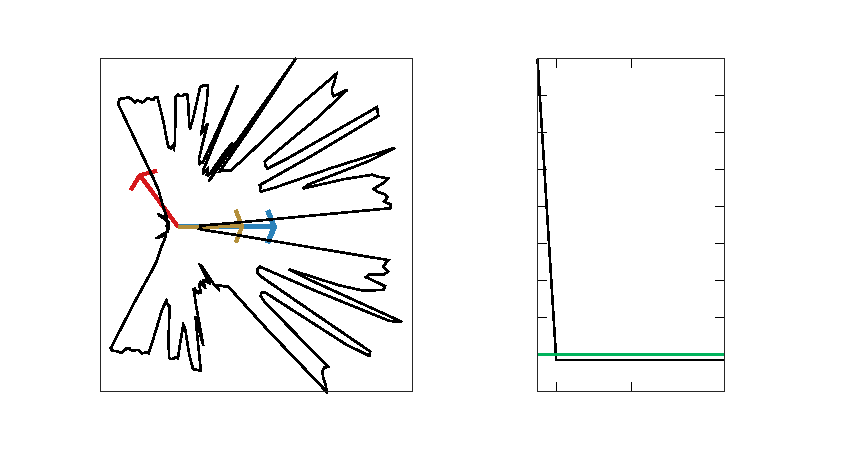
\includegraphics{./figures/parts/02/chapters/04/sections/02/rc_fm}}%
    \gplfronttext
  \end{picture}%
\endgroup

  \vspace{0.5cm}
  \caption{\small Αριστερά: η αρχική
           $\hat{\bm{p}}[0] \equiv (\bm{l},\hat{\theta}[0])$ και τελική
           $\hat{\bm{p}}[1] \equiv (\bm{l},\hat{\theta}[1])$ εκτίμηση στάσης του
           αισθητήρα σε ένα περιβάλλον με χάρτη $\bm{M}$, για πραγματική στάση
           $\bm{p}(\bm{l},\theta)$, ως συνέπεια της εφαρμογής της μεθόδου
           γωνιακής ευθυγράμμισης Fourier-Mellin μίας διάστασης. Δεξιά: το
           σφάλμα εκτίμησης προσανατολισμού ως συνάρτηση της διακριτικής γωνίας
           $\gamma$ του αισθητήρα}
  \label{fig:02_04_02:rc_fm}
\end{figure}

\begin{figure}[h]\centering
  % GNUPLOT: LaTeX picture with Postscript
\begingroup
  \makeatletter
  \providecommand\color[2][]{%
    \GenericError{(gnuplot) \space\space\space\@spaces}{%
      Package color not loaded in conjunction with
      terminal option `colourtext'%
    }{See the gnuplot documentation for explanation.%
    }{Either use 'blacktext' in gnuplot or load the package
      color.sty in LaTeX.}%
    \renewcommand\color[2][]{}%
  }%
  \providecommand\includegraphics[2][]{%
    \GenericError{(gnuplot) \space\space\space\@spaces}{%
      Package graphicx or graphics not loaded%
    }{See the gnuplot documentation for explanation.%
    }{The gnuplot epslatex terminal needs graphicx.sty or graphics.sty.}%
    \renewcommand\includegraphics[2][]{}%
  }%
  \providecommand\rotatebox[2]{#2}%
  \@ifundefined{ifGPcolor}{%
    \newif\ifGPcolor
    \GPcolorfalse
  }{}%
  \@ifundefined{ifGPblacktext}{%
    \newif\ifGPblacktext
    \GPblacktexttrue
  }{}%
  % define a \g@addto@macro without @ in the name:
  \let\gplgaddtomacro\g@addto@macro
  % define empty templates for all commands taking text:
  \gdef\gplfronttext{}%
  \gdef\gplfronttext{}%
  \makeatother
  \ifGPblacktext
    % no textcolor at all
    \def\colorrgb#1{}%
    \def\colorgray#1{}%
  \else
    % gray or color?
    \ifGPcolor
      \def\colorrgb#1{\color[rgb]{#1}}%
      \def\colorgray#1{\color[gray]{#1}}%
      \expandafter\def\csname LTw\endcsname{\color{white}}%
      \expandafter\def\csname LTb\endcsname{\color{black}}%
      \expandafter\def\csname LTa\endcsname{\color{black}}%
      \expandafter\def\csname LT0\endcsname{\color[rgb]{1,0,0}}%
      \expandafter\def\csname LT1\endcsname{\color[rgb]{0,1,0}}%
      \expandafter\def\csname LT2\endcsname{\color[rgb]{0,0,1}}%
      \expandafter\def\csname LT3\endcsname{\color[rgb]{1,0,1}}%
      \expandafter\def\csname LT4\endcsname{\color[rgb]{0,1,1}}%
      \expandafter\def\csname LT5\endcsname{\color[rgb]{1,1,0}}%
      \expandafter\def\csname LT6\endcsname{\color[rgb]{0,0,0}}%
      \expandafter\def\csname LT7\endcsname{\color[rgb]{1,0.3,0}}%
      \expandafter\def\csname LT8\endcsname{\color[rgb]{0.5,0.5,0.5}}%
    \else
      % gray
      \def\colorrgb#1{\color{black}}%
      \def\colorgray#1{\color[gray]{#1}}%
      \expandafter\def\csname LTw\endcsname{\color{white}}%
      \expandafter\def\csname LTb\endcsname{\color{black}}%
      \expandafter\def\csname LTa\endcsname{\color{black}}%
      \expandafter\def\csname LT0\endcsname{\color{black}}%
      \expandafter\def\csname LT1\endcsname{\color{black}}%
      \expandafter\def\csname LT2\endcsname{\color{black}}%
      \expandafter\def\csname LT3\endcsname{\color{black}}%
      \expandafter\def\csname LT4\endcsname{\color{black}}%
      \expandafter\def\csname LT5\endcsname{\color{black}}%
      \expandafter\def\csname LT6\endcsname{\color{black}}%
      \expandafter\def\csname LT7\endcsname{\color{black}}%
      \expandafter\def\csname LT8\endcsname{\color{black}}%
    \fi
  \fi
    \setlength{\unitlength}{0.0500bp}%
    \ifx\gptboxheight\undefined%
      \newlength{\gptboxheight}%
      \newlength{\gptboxwidth}%
      \newsavebox{\gptboxtext}%
    \fi%
    \setlength{\fboxrule}{0.5pt}%
    \setlength{\fboxsep}{1pt}%
\begin{picture}(4800.00,3600.00)%
    \gplgaddtomacro\gplfronttext{%
      \colorrgb{0.15,0.15,0.15}%
      \put(814,1040){\makebox(0,0)[r]{\strut{}$0.4$}}%
      \colorrgb{0.15,0.15,0.15}%
      \put(814,1713){\makebox(0,0)[r]{\strut{}$0.6$}}%
      \colorrgb{0.15,0.15,0.15}%
      \put(814,2386){\makebox(0,0)[r]{\strut{}$0.8$}}%
      \colorrgb{0.15,0.15,0.15}%
      \put(814,3059){\makebox(0,0)[r]{\strut{}$1.0$}}%
      \colorrgb{0.15,0.15,0.15}%
      \put(946,484){\makebox(0,0){\strut{}$360$$\cdot$$2^0$}}%
      \colorrgb{0.15,0.15,0.15}%
      \put(2055,484){\makebox(0,0){\strut{}$360$$\cdot$$2^1$}}%
      \colorrgb{0.15,0.15,0.15}%
      \put(3163,484){\makebox(0,0){\strut{}$360$$\cdot$$2^2$}}%
      \colorrgb{0.15,0.15,0.15}%
      \put(4272,484){\makebox(0,0){\strut{}$360$$\cdot$$2^3$}}%
    }%
    \gplgaddtomacro\gplfronttext{%
      \colorrgb{0.15,0.15,0.15}%
      \put(176,1881){\rotatebox{90}{\makebox(0,0){\strut{}Χρόνος εκτέλεσης [ms]}}}%
      \colorrgb{0.15,0.15,0.15}%
      \put(2609,154){\makebox(0,0){\strut{}Αριθμός ακτίνων $N_s$}}%
      \colorrgb{0.00,0.00,0.00}%
      \put(2609,3269){\makebox(0,0){\strut{}$T_{\texttt{rc\_fm}}$}}%
    }%
    \put(0,0){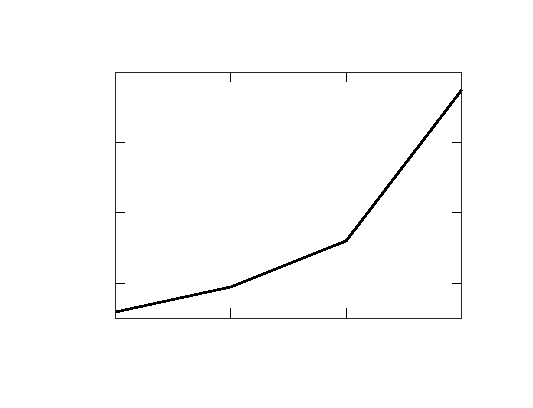
\includegraphics{./figures/parts/02/chapters/04/sections/02/times_rc_fm}}%
    \gplfronttext
  \end{picture}%
\endgroup

  \caption{\small Ο μέσος χρόνος εκτέλεσης μίας επανάληψης της μεθόδου
           Fourier-Mellin μίας διάστασης για δέκα εκτελέσεις, ανά μέγεθος
           σαρώσεων εισόδου $N_s$}
  \label{fig:02_04_02:rc_fm_exec_time}
\end{figure}

\begin{algorithm}[h]
  \caption{\texttt{rc\_fm}}
  \begin{spacing}{1.3}
  \begin{algorithmic}[1]
    \REQUIRE $\mathcal{S}_R$, $\mathcal{S}_V$, $\hat{\bm{p}}(x, y, \hat{\theta})$, $\gamma$
    \ENSURE $\hat{\theta}^\prime$, $q_{\max}$
    \STATE $q_{\mathcal{S}_V, \mathcal{S}_R} \leftarrow \mathcal{F}^{-1}\{Q_{\mathcal{S}_V, \mathcal{S}_R}\}$ (εξ. \ref{eq:Q0})
    \STATE $\xi = \operatorname*{arg\,max} \ q_{\mathcal{S}_V, \mathcal{S}_R}$
    \STATE $q_{\max} \leftarrow q_{\mathcal{S}_V, \mathcal{S}_R}[\xi] = \max q_{\mathcal{S}_V, \mathcal{S}_R}$
    \STATE $\hat{\theta}^\prime \leftarrow \hat{\theta} + \xi \gamma$
    \RETURN $(\hat{\theta}^\prime, q_{\max})$
  \end{algorithmic}
  \end{spacing}
  \label{alg:algorithm_fmrc}
\end{algorithm}


%%%%%%%%%%%%%%%%%%%%%%%%%%%%%%%%%%%%%%%%%%%%%%%%%%%%%%%%%%%%%%%%%%%%%%%%%%%%%%%%
\subsection{Η μέθοδος Πρώτων Αρχών}
\label{subsection:02_04_02:02}

Έστω μία δισδιάστατη σάρωση $\mathcal{S}$ που έχει ληφθεί από τη στάση
$(x,y,\theta)$ σε κάποιο σύστημα συντεταγμένων (Ορισμός \ref{def:lidar}). Έστω
ότι το γωνιακό εύρος της $\mathcal{S}$ είναι $\lambda = 2\pi$. Οι συντεταγμένες
του τελικού σημείου της $n$-οστής ακτίνας της $\mathcal{S}$,
$n=0,1,\dots,N_s-1$, στο σύστημα συντεταγμένων είναι $(x_n,y_n)$:
\begin{align}
  x_n &= x + d_n \cos(\theta + \frac{2 \pi n}{N_s} - \pi) = -d_n \cos(\theta + \frac{2 \pi n}{N_s}) \label{eq:x_n}\\
  y_n &= y + d_n \sin(\theta + \frac{2 \pi n}{N_s} - \pi) = -d_n \sin(\theta + \frac{2 \pi n}{N_s}) \label{eq:y_n}
\end{align}
Εδώ παρατηρούμε ότι $-(x_n-x)$ και $(y_n-y)$ είναι αντίστοιχα το πραγματικό και
το φανταστικό μέρος της μιγαδικής ποσότητας
\begin{align}
  d_n e^{-i(\theta + \frac{2 \pi n}{N_s})} &= d_n \cos(\theta + \frac{2 \pi n}{N_s}) - i \cdot d_n \sin(\theta + \frac{2 \pi n}{N}) \nonumber \\
                                         &\leftstackrel{(\ref{eq:x_n}),(\ref{eq:y_n})}{=} -(x_n-x) + i \cdot (y_n-y) \label{eq:dne_complex_x_y}
\end{align}
και, επομένως
\begin{align}
  d_n e^{-i 2 \pi n/N_s} &= e^{i\theta}(-(x_n-x) + i \cdot (y_n-y)) \label{eq:dne_complex}
\end{align}
Αθροίζοντας τα δύο μέλη της εξίσωσης (\ref{eq:dne_complex}) επί του συνόλου των
$N_s$ ακτίνων λαμβάνουμε τον πρώτο όρο του διακριτού μετασχηματισμού Fourier
του σήματος $\{d_n\}$, $n=0,1,\dots,N_s-1$,
$\mathcal{F}_1\{\mathcal{S}\} = \mathcal{F}\{\mathcal{S}\}[1]$:
\begin{align}
  \mathcal{F}_1\{\mathcal{S}\} = \sum\limits_{n=0}^{N_s-1}d_n \cdot e^{-i 2 \pi n/N_s} \ &\leftstackrel{(\ref{eq:dne_complex})}{=} \ \sum\limits_{n=0}^{N_s-1} e^{i\theta}(-(x_n-x) + i \cdot (y_n-y)) \nonumber  \\
           &= e^{i\theta} \sum\limits_{n=0}^{N_s-1} [ (x- i \cdot y) + (-x_n + i \cdot y_n) ]\nonumber \\
           &= e^{i\theta} N_s (x-i\cdot y) - e^{i\theta}\Delta \label{eq:F1}
\end{align}
όπου $\Delta \triangleq \sum\limits_{n=0}^{N_s-1} (x_n -i \cdot y_n)$.

Συμβολίζοντας με το γράμμα $R$ τις ποσότητες που αντιστοιχούν στην πραγματική
σάρωση $\mathcal{S}_R$, η οποία έχει ληφθεί από τη στάση του φυσικού αισθητήρα
$\bm{p}(x,y,\theta)$, και με $V$ εκείνες που αντιστοιχούν στην εικονική σάρωση
$\mathcal{S}_V$, η οποία έχει ληφθεί από τη στάση
$\hat{\bm{p}}(x,y,\hat{\theta})$:
\begin{align}
  \mathcal{F}_1\{\mathcal{S}_R\} &= \sum\limits_{n=0}^{N_s-1}d_n^R \cdot e^{-i 2 \pi n/N_s} \stackrel{(\ref{eq:F1})}{=} N_s e^{i\theta}(x-i\cdot y) - e^{i\theta} \Delta_R \label{eq:dne_complex_r} \\
  \mathcal{F}_1\{\mathcal{S}_V\} &= \sum\limits_{n=0}^{N_s-1}d_n^V \cdot e^{-i 2 \pi n/N_s} \stackrel{(\ref{eq:F1})}{=} N_s e^{i\hat{\theta}}(x-i\cdot y) - e^{i\hat{\theta}} \Delta_V \label{eq:dne_complex_v}
\end{align}

Έστω τώρα ότι
\begin{align}
  \Delta_R - \Delta_V &= \sum\limits_{n=0}^{N_s-1}(x_n^R-x_n^V) - i \cdot \sum\limits_{n=0}^{N_s-1}(y_n^R-y_n^V) \nonumber \\
                      &= N_s (\delta_x - i \cdot \delta_y)
\end{align}
όπου
\begin{align}
  \delta_x &\triangleq \frac{1}{N_s}\sum\limits_{n=0}^{N_s-1}(x_n^R-x_n^V) \label{eq:delta_x}\\
  \delta_y &\triangleq \frac{1}{N_s}\sum\limits_{n=0}^{N_s-1}(y_n^R-y_n^V) \label{eq:delta_y}
\end{align}
τότε
\begin{align}
  \Delta_V &= \Delta_R -N_s(\delta_x - i \cdot \delta_y) \label{eq:Delta_V_eq_Delta_R}
\end{align}

Ο πρώτος όρος του διακριτού μετασχηματισμού Fourier του σήματος που
αποτελείται από τη διαφορά των δύο σημάτων (\ref{eq:dne_complex_r}) και
(\ref{eq:dne_complex_v}) είναι:
\begin{align}
  \mathcal{F}_1\{\mathcal{S}_R\} - \mathcal{F}_1\{\mathcal{S}_V\} &= \sum\limits_{n=0}^{N_s-1}(d_n^R - d_n^V) \cdot e^{-i 2 \pi n/N_s} \nonumber \\
           &\leftstackrel{(\ref{eq:dne_complex_r}),(\ref{eq:dne_complex_v})}{=} N_s (x-i \cdot y)(e^{i\theta}-e^{i\hat{\theta}}) -e^{i\theta}\Delta_R+e^{i\hat{\theta}}\Delta_V \nonumber \\
          &\leftstackrel{(\ref{eq:Delta_V_eq_Delta_R})}{=} N_s (x-i \cdot y)(e^{i\theta}-e^{i\hat{\theta}}) -e^{i\theta}\Delta_R +e^{i\hat{\theta}}(\Delta_R -N_s(\delta_x - i \cdot \delta_y)) \nonumber \\
          &= N_s (x-i \cdot y)(e^{i\theta}-e^{i\hat{\theta}}) - \Delta_R (e^{i\theta}-e^{i\hat{\theta}})- N_s e^{i\hat{\theta}}(\delta_x - i\cdot \delta_y) \nonumber \\
          &= (e^{i\theta}-e^{i\hat{\theta}}) [N_s(x-i\cdot y) - \Delta_R]- N_s e^{i\hat{\theta}}(\delta_x - i\cdot \delta_y) \nonumber   \\
          &\leftstackrel{(\ref{eq:dne_complex_r})}{=} (e^{i\theta}-e^{i\hat{\theta}}) \dfrac{\mathcal{F}_1\{\mathcal{S}_R\}}{e^{i\theta}}- N_s e^{i\hat{\theta}}(\delta_x - i\cdot \delta_y) \nonumber \\
          &= (1-e^{-i(\theta-\hat{\theta})}) \mathcal{F}_1\{\mathcal{S}_R\}- N_s e^{i\hat{\theta}}(\delta_x - i\cdot \delta_y) \nonumber
\end{align}
άρα
\begin{align}
  -\mathcal{F}_1\{\mathcal{S}_V\} &= -e^{-i(\theta-\hat{\theta})} \mathcal{F}_1\{\mathcal{S}_R\}- N_s e^{i\hat{\theta}}(\delta_x - i\cdot \delta_y) \label{eq:x1_for_proof} \\
  e^{-i(\theta-\hat{\theta})} &= \dfrac{\mathcal{F}_1\{\mathcal{S}_V\}}{\mathcal{F}_1\{\mathcal{S}_R\}} - \dfrac{N_s e^{i\hat{\theta}}}{\mathcal{F}_1\{\mathcal{S}_R\}}(\delta_x - i\cdot \delta_y) \nonumber
\end{align}
Χρησιμοποιώντας την πολική αναπαράσταση $\bm{A} = |\bm{A}| e^{i\angle \bm{A}}$:
\begin{align}
  e^{-i(\theta-\hat{\theta})} &= \dfrac{|\mathcal{F}_1\{\mathcal{S}_V\}|}{|\mathcal{F}_1\{\mathcal{S}_R\}|} e^{-i(\angle \mathcal{F}_1\{\mathcal{S}_R\} - \angle \mathcal{F}_1\{\mathcal{S}_V\})} - \dfrac{e^{-i(\angle \mathcal{F}_1\{\mathcal{S}_R\}-\hat{\theta})}}{|\mathcal{F}_1\{\mathcal{S}_R\}|} (N_s \delta_x - i\cdot N_s \delta_y) \label{eq:x1_final_big_eq}
\end{align}

Λόγω του γεγονότος ότι ο προσανατολισμός $\theta$ του αισθητήρα είναι άγνωστος,
τα τελικά σημεία $\{(x_n^R,y_n^R)\}$ καθίστανται ομοίως άγνωστα, και συνεπώς
και οι ποσότητες $\delta_x, \delta_y$. Προκειμένου να αποκτήσουμε μια αρχική
διαίσθηση ως προς τα μέτρα των τελευταίων κάνουμε την παρατήρηση ότι, εξ
ορισμού, οι ποσότητες $N_s \delta_x$ και $N_s \delta_y$ ποσοτικοποιούν τη
διαφορά της προσέγγισης των επικαμπύλιων ολοκληρωμάτων επί των καμπύλων που
ορίζονται από τα τελικά σημεία των δύο σαρώσεων στους δύο κύριους άξονες $x$
και $y$.  Η προσέγγιση αυτή οφείλεται στο πεπερασμένο μέγεθος των εκπεμπόμενων
ακτίνων $N_s$. Επομένως υπό τις υποθέσεις ότι (α) ο χάρτης του περιβάλλοντος
είναι τέλεια αναπαράστασή του και (β) οι μετρήσεις του φυσικού αισθητήρα δεν
επηρεάζονται από διαταραχές: καθώς $N_s \rightarrow \infty$, $N_s \delta_x$,
$N_s \delta_y$ $\rightarrow 0$, τα οποία με τη σειρά τους σημαίνουν λόγω της
εξίσωσης (\ref{eq:x1_final_big_eq}) ότι
$\dfrac{|\mathcal{F}_1\{\mathcal{S}_V\}|}{|\mathcal{F}_1\{\mathcal{S}_R\}|}
\rightarrow 1$ και $\theta-\hat{\theta} \rightarrow \angle
\mathcal{F}_1\{\mathcal{S}_R\} - \angle \mathcal{F}_1\{\mathcal{S}_V\}$.
Η παραπάνω ανάλυση μάς οδηγεί στη διατύπωση του Λήμματος \ref{lemma:02_04_02:02}:

\begin{lemma}
  Έστω οι παραδοχές του προβλήματος \ref{prob:02_04} και $\hat{\bm{l}} = \bm{l}$.
  Έστω επίσης ότι (α) οι μετρήσεις του φυσικού αισθητήρα δεν φέρουν
  διαταραχές, και (β) ο χάρτης $\bm{M}$ αναπαριστά το περιβάλλον τέλεια. Τότε
  ενημερώνοντας την εκτίμηση προσανατολισμού σε $\hat{\theta}^\prime$:
  \begin{align}
  \hat{\theta}^\prime = \hat{\theta} + \angle \mathcal{F}_1\{\mathcal{S}_R\} - \angle\mathcal{F}_1\{\mathcal{S}_V\}
    \label{eq:update_t2}
  \end{align}
  όπου $\mathcal{F}_1\{\cdot\} = \mathcal{F}\{\cdot\} [1]$,
  οδηγεί σε ένα επίλοιπο σφάλμα προσανατολισμού $\phi$:
  \begin{align}
    \phi &= \angle \mathcal{F}_1\{\mathcal{S}_V\} - \tan^{-1}\dfrac{|\mathcal{F}_1\{\mathcal{S}_V\}| \sin(\angle \mathcal{F}_1\{\mathcal{S}_V\})-N_s |\delta| \sin(\hat{\theta} + \angle \delta)}
                                                                 {|\mathcal{F}_1\{\mathcal{S}_V\}| \cos(\angle \mathcal{F}_1\{\mathcal{S}_V\})-N_s |\delta| \cos(\hat{\theta} + \angle \delta)} \label{eq:phi2}
  \end{align}
  όπου $\delta = \delta_x - i \cdot \delta_y$.
  \label{lemma:02_04_02:02}
\end{lemma}

Η απόδειξη βρίσκεται στο παράρτημα \ref{appendix:04:lemma_01_proof}.

\begin{corollary}
  Το μέτρο του σφάλματος $|\phi|$ είναι αντιστρόφως ανάλογο του αριθμού των
  ακτίνων $N_s$ που εκπέμπει ο αισθητήρας στην περίπτωση που τόσο η πραγματική
  μέτρηση $\mathcal{S}_R$ όσο και η εικονική σάρωση $\mathcal{S}_V$ δεν
  διαταράσσονται από θόρυβο (σχήμα \ref{fig:02_04_02:phi_rc_x1}).
\end{corollary}


\begin{figure}[h]\centering
  \vspace{0.5cm}
  % GNUPLOT: LaTeX picture with Postscript
\begingroup
  \makeatletter
  \providecommand\color[2][]{%
    \GenericError{(gnuplot) \space\space\space\@spaces}{%
      Package color not loaded in conjunction with
      terminal option `colourtext'%
    }{See the gnuplot documentation for explanation.%
    }{Either use 'blacktext' in gnuplot or load the package
      color.sty in LaTeX.}%
    \renewcommand\color[2][]{}%
  }%
  \providecommand\includegraphics[2][]{%
    \GenericError{(gnuplot) \space\space\space\@spaces}{%
      Package graphicx or graphics not loaded%
    }{See the gnuplot documentation for explanation.%
    }{The gnuplot epslatex terminal needs graphicx.sty or graphics.sty.}%
    \renewcommand\includegraphics[2][]{}%
  }%
  \providecommand\rotatebox[2]{#2}%
  \@ifundefined{ifGPcolor}{%
    \newif\ifGPcolor
    \GPcolorfalse
  }{}%
  \@ifundefined{ifGPblacktext}{%
    \newif\ifGPblacktext
    \GPblacktexttrue
  }{}%
  % define a \g@addto@macro without @ in the name:
  \let\gplgaddtomacro\g@addto@macro
  % define empty templates for all commands taking text:
  \gdef\gplfronttext{}%
  \gdef\gplfronttext{}%
  \makeatother
  \ifGPblacktext
    % no textcolor at all
    \def\colorrgb#1{}%
    \def\colorgray#1{}%
  \else
    % gray or color?
    \ifGPcolor
      \def\colorrgb#1{\color[rgb]{#1}}%
      \def\colorgray#1{\color[gray]{#1}}%
      \expandafter\def\csname LTw\endcsname{\color{white}}%
      \expandafter\def\csname LTb\endcsname{\color{black}}%
      \expandafter\def\csname LTa\endcsname{\color{black}}%
      \expandafter\def\csname LT0\endcsname{\color[rgb]{1,0,0}}%
      \expandafter\def\csname LT1\endcsname{\color[rgb]{0,1,0}}%
      \expandafter\def\csname LT2\endcsname{\color[rgb]{0,0,1}}%
      \expandafter\def\csname LT3\endcsname{\color[rgb]{1,0,1}}%
      \expandafter\def\csname LT4\endcsname{\color[rgb]{0,1,1}}%
      \expandafter\def\csname LT5\endcsname{\color[rgb]{1,1,0}}%
      \expandafter\def\csname LT6\endcsname{\color[rgb]{0,0,0}}%
      \expandafter\def\csname LT7\endcsname{\color[rgb]{1,0.3,0}}%
      \expandafter\def\csname LT8\endcsname{\color[rgb]{0.5,0.5,0.5}}%
    \else
      % gray
      \def\colorrgb#1{\color{black}}%
      \def\colorgray#1{\color[gray]{#1}}%
      \expandafter\def\csname LTw\endcsname{\color{white}}%
      \expandafter\def\csname LTb\endcsname{\color{black}}%
      \expandafter\def\csname LTa\endcsname{\color{black}}%
      \expandafter\def\csname LT0\endcsname{\color{black}}%
      \expandafter\def\csname LT1\endcsname{\color{black}}%
      \expandafter\def\csname LT2\endcsname{\color{black}}%
      \expandafter\def\csname LT3\endcsname{\color{black}}%
      \expandafter\def\csname LT4\endcsname{\color{black}}%
      \expandafter\def\csname LT5\endcsname{\color{black}}%
      \expandafter\def\csname LT6\endcsname{\color{black}}%
      \expandafter\def\csname LT7\endcsname{\color{black}}%
      \expandafter\def\csname LT8\endcsname{\color{black}}%
    \fi
  \fi
    \setlength{\unitlength}{0.0500bp}%
    \ifx\gptboxheight\undefined%
      \newlength{\gptboxheight}%
      \newlength{\gptboxwidth}%
      \newsavebox{\gptboxtext}%
    \fi%
    \setlength{\fboxrule}{0.5pt}%
    \setlength{\fboxsep}{1pt}%
\begin{picture}(5000.00,4000.00)%
    \gplgaddtomacro\gplfronttext{%
      \put(1078,0){\makebox(0,0){\strut{}$-\pi$}}%
      \colorrgb{0.15,0.15,0.15}%
      \put(1959,0){\makebox(0,0){\strut{}$-\dfrac{\pi}{2}$}}%
      \colorrgb{0.15,0.15,0.15}%
      \put(2841,0){\makebox(0,0){\strut{}$0$}}%
      \colorrgb{0.15,0.15,0.15}%
      \put(3722,0){\makebox(0,0){\strut{}$+\dfrac{\pi}{2}$}}%
      \colorrgb{0.15,0.15,0.15}%
      \put(4603,0){\makebox(0,0){\strut{}$+\pi$}}%
      \colorrgb{0.15,0.15,0.15}%
      \put(946,264){\makebox(0,0)[r]{\strut{}$10^{-4}$}}%
      \colorrgb{0.15,0.15,0.15}%
      \put(946,743){\makebox(0,0)[r]{\strut{}$10^{-3}$}}%
      \colorrgb{0.15,0.15,0.15}%
      \put(946,1222){\makebox(0,0)[r]{\strut{}$10^{-2}$}}%
      \colorrgb{0.15,0.15,0.15}%
      \put(946,1701){\makebox(0,0)[r]{\strut{}$10^{-1}$}}%
      \colorrgb{0.15,0.15,0.15}%
      \put(946,2181){\makebox(0,0)[r]{\strut{}$10^{0}$}}%
      \colorrgb{0.15,0.15,0.15}%
      \put(946,2660){\makebox(0,0)[r]{\strut{}$10^{1}$}}%
      \colorrgb{0.15,0.15,0.15}%
      \put(946,3139){\makebox(0,0)[r]{\strut{}$10^{2}$}}%
      \colorrgb{0.15,0.15,0.15}%
      \put(1078,3359){\makebox(0,0){\strut{}$-\pi$}}%
      \colorrgb{0.15,0.15,0.15}%
      \put(1959,3359){\makebox(0,0){\strut{}$-\dfrac{\pi}{2}$}}%
      \colorrgb{0.15,0.15,0.15}%
      \put(2841,3359){\makebox(0,0){\strut{}$0$}}%
      \colorrgb{0.15,0.15,0.15}%
      \put(3722,3359){\makebox(0,0){\strut{}$+\dfrac{\pi}{2}$}}%
      \colorrgb{0.15,0.15,0.15}%
      \put(4603,3359){\makebox(0,0){\strut{}$+\pi$}}%
    }%
    \gplgaddtomacro\gplfronttext{%
      \colorrgb{0.15,0.15,0.15}%
      \put(176,1701){\rotatebox{90}{\makebox(0,0){\strut{}$N_s |\delta|$ [m]}}}%
      \colorrgb{0.00,0.00,0.00}%
      \put(2840,3889){\makebox(0,0){\strut{}Επίλοιπο σφάλμα $\phi$: εξ. (\ref{eq:phi2})}}%
      \colorrgb{0.15,0.15,0.15}%
      \put(2840,-400){\makebox(0,0){\strut{}$\phi$ [rad]}}%
    }%
    \put(0,0){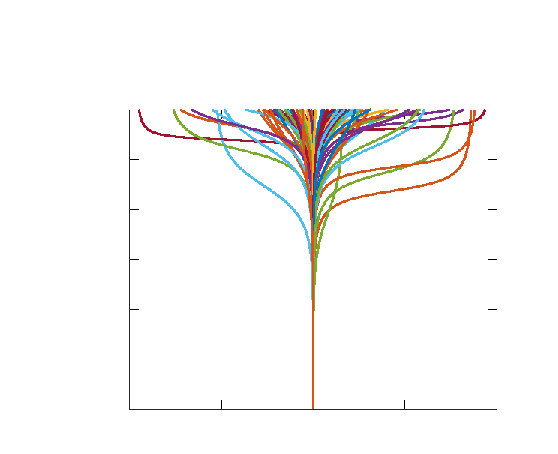
\includegraphics{./figures/parts/02/chapters/04/sections/02/phi_rc_x1}}%
    \gplfronttext
  \end{picture}%
\endgroup

  \vspace{1.0cm}
  \caption{\small Θεωρητικές τιμές του επίλοιπου σφάλματος $\phi$ (εξ.
           \ref{eq:phi2}) σε εκατό προσομοιώσεις για μεταβλητές τιμές
           $N_s |\delta|$. Το μέτρο $|\mathcal{F}_1\{\mathcal{S}_V\}|$ είναι
           ομοιόμορφα κατανεμημένο στο διάστημα $[0.0, 200.0]$, το μέγεθος
           $N_s |\delta|$ στο διάστημα $[10^{-4}, 10^{+2}]$, και τα ορίσματα
           $\angle \mathcal{F}_1\{\mathcal{S}_V\}$, $\angle \delta$ στο
           $[-\pi, \pi)$. Το επίλοιπο σφάλμα $\phi \rightarrow 0$ καθώς
           $N_s \rightarrow \infty \Rightarrow N_s |\delta| \rightarrow 0$}
  \label{fig:02_04_02:phi_rc_x1}
\end{figure}

Η παραπάνω μέθοδος εκτίμησης του προσανατολισμού της στάσης
$\bm{p}(x,y,\theta)$ ονομάζεται στο εξής μέθοδος Πρώτων Αρχών.  Στο σχήμα
\ref{fig:02_04_02:rc_x1} απεικονίζεται η αρχική και τελική συνθήκη
ευθυγράμμισης προσανατολισμού με εφαρμογή της μεθόδου Πρώτων αρχών για έναν
αισθητήρα δισδιάστατων πανοραμικών σαρώσεων με $\gamma = 2\pi/360$, υπό τις
ίδιες συνθήκες διεξαγωγής μείωσης του σφάλματος προσανατολισμού με αυτές που
παρουσιάζονται στο σχήμα \ref{fig:02_04_02:rc_fm}. Το σχήμα
\ref{fig:02_04_02:rc_x1_exec_time} απεικονίζει το μέσο χρόνο εκτέλεσης
μίας επανάληψης της μεθόδου σε δέκα εκτελέσεις για αυξανόμενο μέγεθος σαρώσεων
$N_s$. Ο Αλγόριθμος \ref{alg:algorithm_x1rc} παρουσιάζει σε ψευδοκώδικα τη
διαδικασία διόρθωσης προσανατολισμού με βάση την εν λόγω μέθοδο.

\begin{figure}[h]\centering
  % GNUPLOT: LaTeX picture with Postscript
\begingroup
  \makeatletter
  \providecommand\color[2][]{%
    \GenericError{(gnuplot) \space\space\space\@spaces}{%
      Package color not loaded in conjunction with
      terminal option `colourtext'%
    }{See the gnuplot documentation for explanation.%
    }{Either use 'blacktext' in gnuplot or load the package
      color.sty in LaTeX.}%
    \renewcommand\color[2][]{}%
  }%
  \providecommand\includegraphics[2][]{%
    \GenericError{(gnuplot) \space\space\space\@spaces}{%
      Package graphicx or graphics not loaded%
    }{See the gnuplot documentation for explanation.%
    }{The gnuplot epslatex terminal needs graphicx.sty or graphics.sty.}%
    \renewcommand\includegraphics[2][]{}%
  }%
  \providecommand\rotatebox[2]{#2}%
  \@ifundefined{ifGPcolor}{%
    \newif\ifGPcolor
    \GPcolorfalse
  }{}%
  \@ifundefined{ifGPblacktext}{%
    \newif\ifGPblacktext
    \GPblacktexttrue
  }{}%
  % define a \g@addto@macro without @ in the name:
  \let\gplgaddtomacro\g@addto@macro
  % define empty templates for all commands taking text:
  \gdef\gplfronttext{}%
  \gdef\gplfronttext{}%
  \makeatother
  \ifGPblacktext
    % no textcolor at all
    \def\colorrgb#1{}%
    \def\colorgray#1{}%
  \else
    % gray or color?
    \ifGPcolor
      \def\colorrgb#1{\color[rgb]{#1}}%
      \def\colorgray#1{\color[gray]{#1}}%
      \expandafter\def\csname LTw\endcsname{\color{white}}%
      \expandafter\def\csname LTb\endcsname{\color{black}}%
      \expandafter\def\csname LTa\endcsname{\color{black}}%
      \expandafter\def\csname LT0\endcsname{\color[rgb]{1,0,0}}%
      \expandafter\def\csname LT1\endcsname{\color[rgb]{0,1,0}}%
      \expandafter\def\csname LT2\endcsname{\color[rgb]{0,0,1}}%
      \expandafter\def\csname LT3\endcsname{\color[rgb]{1,0,1}}%
      \expandafter\def\csname LT4\endcsname{\color[rgb]{0,1,1}}%
      \expandafter\def\csname LT5\endcsname{\color[rgb]{1,1,0}}%
      \expandafter\def\csname LT6\endcsname{\color[rgb]{0,0,0}}%
      \expandafter\def\csname LT7\endcsname{\color[rgb]{1,0.3,0}}%
      \expandafter\def\csname LT8\endcsname{\color[rgb]{0.5,0.5,0.5}}%
    \else
      % gray
      \def\colorrgb#1{\color{black}}%
      \def\colorgray#1{\color[gray]{#1}}%
      \expandafter\def\csname LTw\endcsname{\color{white}}%
      \expandafter\def\csname LTb\endcsname{\color{black}}%
      \expandafter\def\csname LTa\endcsname{\color{black}}%
      \expandafter\def\csname LT0\endcsname{\color{black}}%
      \expandafter\def\csname LT1\endcsname{\color{black}}%
      \expandafter\def\csname LT2\endcsname{\color{black}}%
      \expandafter\def\csname LT3\endcsname{\color{black}}%
      \expandafter\def\csname LT4\endcsname{\color{black}}%
      \expandafter\def\csname LT5\endcsname{\color{black}}%
      \expandafter\def\csname LT6\endcsname{\color{black}}%
      \expandafter\def\csname LT7\endcsname{\color{black}}%
      \expandafter\def\csname LT8\endcsname{\color{black}}%
    \fi
  \fi
    \setlength{\unitlength}{0.0500bp}%
    \ifx\gptboxheight\undefined%
      \newlength{\gptboxheight}%
      \newlength{\gptboxwidth}%
      \newsavebox{\gptboxtext}%
    \fi%
    \setlength{\fboxrule}{0.5pt}%
    \setlength{\fboxsep}{1pt}%
\begin{picture}(4800.00,3600.00)%
    \gplgaddtomacro\gplfronttext{%
      \colorrgb{0.15,0.15,0.15}%
      \put(946,704){\makebox(0,0)[r]{\strut{}$0.02$}}%
      \colorrgb{0.15,0.15,0.15}%
      \put(946,1377){\makebox(0,0)[r]{\strut{}$0.06$}}%
      \colorrgb{0.15,0.15,0.15}%
      \put(946,2050){\makebox(0,0)[r]{\strut{}$0.10$}}%
      \colorrgb{0.15,0.15,0.15}%
      \put(946,2723){\makebox(0,0)[r]{\strut{}$0.14$}}%
      \colorrgb{0.15,0.15,0.15}%
      \put(1078,484){\makebox(0,0){\strut{}$360$$\cdot$$2^0$}}%
      \colorrgb{0.15,0.15,0.15}%
      \put(2143,484){\makebox(0,0){\strut{}$360$$\cdot$$2^1$}}%
      \colorrgb{0.15,0.15,0.15}%
      \put(3207,484){\makebox(0,0){\strut{}$360$$\cdot$$2^2$}}%
      \colorrgb{0.15,0.15,0.15}%
      \put(4272,484){\makebox(0,0){\strut{}$360$$\cdot$$2^3$}}%
    }%
    \gplgaddtomacro\gplfronttext{%
      \colorrgb{0.15,0.15,0.15}%
      \put(176,1881){\rotatebox{90}{\makebox(0,0){\strut{}Χρόνος εκτέλεσης [ms]}}}%
      \colorrgb{0.15,0.15,0.15}%
      \put(2675,154){\makebox(0,0){\strut{}Αριθμός ακτίνων $N_s$}}%
      \colorrgb{0.00,0.00,0.00}%
      \put(2675,3269){\makebox(0,0){\strut{}$T_{\texttt{rc\_x1}}$}}%
    }%
    \put(0,0){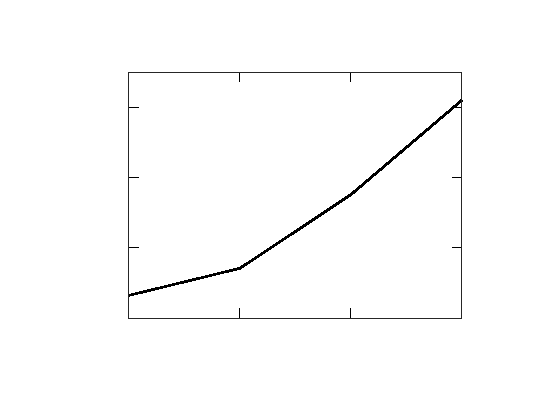
\includegraphics{./figures/parts/02/chapters/04/sections/02/times_rc_x1}}%
    \gplfronttext
  \end{picture}%
\endgroup

  \caption{\small Ο μέσος χρόνος εκτέλεσης μίας επανάληψης της μεθόδου
           Πρώτων Αρχών για δέκα εκτελέσεις, ανά μέγεθος σαρώσεων εισόδου $N_s$}
  \label{fig:02_04_02:rc_x1_exec_time}
\end{figure}

\begin{figure}[h]\centering
  \vspace{0.5cm}
  \definecolor{sr}{RGB}{43,131,186}
\definecolor{svi}{RGB}{215,25, 28}
\definecolor{svf}{RGB}{179,143,59}
\definecolor{g}{RGB}{0,178,93}
\definecolor{k}{RGB}{0,0,0}

% GNUPLOT: LaTeX picture with Postscript
\begingroup
  \makeatletter
  \providecommand\color[2][]{%
    \GenericError{(gnuplot) \space\space\space\@spaces}{%
      Package color not loaded in conjunction with
      terminal option `colourtext'%
    }{See the gnuplot documentation for explanation.%
    }{Either use 'blacktext' in gnuplot or load the package
      color.sty in LaTeX.}%
    \renewcommand\color[2][]{}%
  }%
  \providecommand\includegraphics[2][]{%
    \GenericError{(gnuplot) \space\space\space\@spaces}{%
      Package graphicx or graphics not loaded%
    }{See the gnuplot documentation for explanation.%
    }{The gnuplot epslatex terminal needs graphicx.sty or graphics.sty.}%
    \renewcommand\includegraphics[2][]{}%
  }%
  \providecommand\rotatebox[2]{#2}%
  \@ifundefined{ifGPcolor}{%
    \newif\ifGPcolor
    \GPcolorfalse
  }{}%
  \@ifundefined{ifGPblacktext}{%
    \newif\ifGPblacktext
    \GPblacktexttrue
  }{}%
  % define a \g@addto@macro without @ in the name:
  \let\gplgaddtomacro\g@addto@macro
  % define empty templates for all commands taking text:
  \gdef\gplfronttext{}%
  \gdef\gplfronttext{}%
  \makeatother
  \ifGPblacktext
    % no textcolor at all
    \def\colorrgb#1{}%
    \def\colorgray#1{}%
  \else
    % gray or color?
    \ifGPcolor
      \def\colorrgb#1{\color[rgb]{#1}}%
      \def\colorgray#1{\color[gray]{#1}}%
      \expandafter\def\csname LTw\endcsname{\color{white}}%
      \expandafter\def\csname LTb\endcsname{\color{black}}%
      \expandafter\def\csname LTa\endcsname{\color{black}}%
      \expandafter\def\csname LT0\endcsname{\color[rgb]{1,0,0}}%
      \expandafter\def\csname LT1\endcsname{\color[rgb]{0,1,0}}%
      \expandafter\def\csname LT2\endcsname{\color[rgb]{0,0,1}}%
      \expandafter\def\csname LT3\endcsname{\color[rgb]{1,0,1}}%
      \expandafter\def\csname LT4\endcsname{\color[rgb]{0,1,1}}%
      \expandafter\def\csname LT5\endcsname{\color[rgb]{1,1,0}}%
      \expandafter\def\csname LT6\endcsname{\color[rgb]{0,0,0}}%
      \expandafter\def\csname LT7\endcsname{\color[rgb]{1,0.3,0}}%
      \expandafter\def\csname LT8\endcsname{\color[rgb]{0.5,0.5,0.5}}%
    \else
      % gray
      \def\colorrgb#1{\color{black}}%
      \def\colorgray#1{\color[gray]{#1}}%
      \expandafter\def\csname LTw\endcsname{\color{white}}%
      \expandafter\def\csname LTb\endcsname{\color{black}}%
      \expandafter\def\csname LTa\endcsname{\color{black}}%
      \expandafter\def\csname LT0\endcsname{\color{black}}%
      \expandafter\def\csname LT1\endcsname{\color{black}}%
      \expandafter\def\csname LT2\endcsname{\color{black}}%
      \expandafter\def\csname LT3\endcsname{\color{black}}%
      \expandafter\def\csname LT4\endcsname{\color{black}}%
      \expandafter\def\csname LT5\endcsname{\color{black}}%
      \expandafter\def\csname LT6\endcsname{\color{black}}%
      \expandafter\def\csname LT7\endcsname{\color{black}}%
      \expandafter\def\csname LT8\endcsname{\color{black}}%
    \fi
  \fi
    \setlength{\unitlength}{0.0500bp}%
    \ifx\gptboxheight\undefined%
      \newlength{\gptboxheight}%
      \newlength{\gptboxwidth}%
      \newsavebox{\gptboxtext}%
    \fi%
    \setlength{\fboxrule}{0.5pt}%
    \setlength{\fboxsep}{1pt}%
\begin{picture}(8000.00,4000.00)%
    \gplgaddtomacro\gplfronttext{%
    }%
    \gplgaddtomacro\gplfronttext{%
    }%
    \gplgaddtomacro\gplfronttext{%
      \colorrgb{0.15,0.15,0.15}%
      \put(4868,647){\makebox(0,0)[r]{\strut{}$2^{-3}$}}%
      \colorrgb{0.15,0.15,0.15}%
      \put(4868,942){\makebox(0,0)[r]{\strut{}$2^{-2}$}}%
      \colorrgb{0.15,0.15,0.15}%
      \put(4868,1237){\makebox(0,0)[r]{\strut{}$2^{-1}$}}%
      \colorrgb{0.15,0.15,0.15}%
      \put(4868,1533){\makebox(0,0)[r]{\strut{}$2^{0}$}}%
      \colorrgb{0.15,0.15,0.15}%
      \put(4868,1828){\makebox(0,0)[r]{\strut{}$2^{1}$}}%
      \colorrgb{0.15,0.15,0.15}%
      \put(4868,2123){\makebox(0,0)[r]{\strut{}$2^{2}$}}%
      \colorrgb{0.15,0.15,0.15}%
      \put(4868,2418){\makebox(0,0)[r]{\strut{}$2^{3}$}}%
      \colorrgb{0.15,0.15,0.15}%
      \put(4868,2713){\makebox(0,0)[r]{\strut{}$2^{4}$}}%
      \colorrgb{0.15,0.15,0.15}%
      \put(4868,3009){\makebox(0,0)[r]{\strut{}$2^{5}$}}%
      \colorrgb{0.15,0.15,0.15}%
      \put(4868,3304){\makebox(0,0)[r]{\strut{}$2^{6}$}}%
      \colorrgb{0.15,0.15,0.15}%
      \put(4868,3599){\makebox(0,0)[r]{\strut{}$2^{7}$}}%
      \colorrgb{0.15,0.15,0.15}%
      \put(5180,180){\makebox(0,0){\strut{}$1$}}%
      \colorrgb{0.15,0.15,0.15}%
      \put(5900,180){\makebox(0,0){\strut{}$5$}}%
      \colorrgb{0.15,0.15,0.15}%
      \put(6799,180){\makebox(0,0){\strut{}$10$}}%
    }%
    \gplgaddtomacro\gplfronttext{%
      \colorrgb{0.15,0.15,0.15}%
      \put(5500,3819){\makebox(0,0){\strut{}{\color{k}{\rule[0.6mm]{0.5cm}{0.5mm}}} $|e_\theta|/\gamma$}}%
      \put(6500,3819){\makebox(0,0){\strut{}{\color{g}{\rule[0.6mm]{0.5cm}{0.5mm}}} $2^{-1}$}}%
      \put(5899,-150){\makebox(0,0){\strut{}Αριθμός επαναλήψεων}}%

      \put(1100,3819){\makebox(0,0){\strut{}{\color{k}{\rule[0.6mm]{0.5cm}{0.5mm}}} $\bm{M}$}}%
      \put(1850,3819){\makebox(0,0){\strut{}{\color{sr}{\rule[0.6mm]{0.5cm}{0.5mm}}} $\bm{p}$}}%
      \put(2600,3819){\makebox(0,0){\strut{}{\color{svi}{\rule[0.6mm]{0.5cm}{0.5mm}}} $\hat{\bm{p}}[0]$}}%
      \put(3500,3819){\makebox(0,0){\strut{}{\color{svf}{\rule[0.6mm]{0.5cm}{0.5mm}}} $\hat{\bm{p}}[10]$}}%
    }%
    \put(0,0){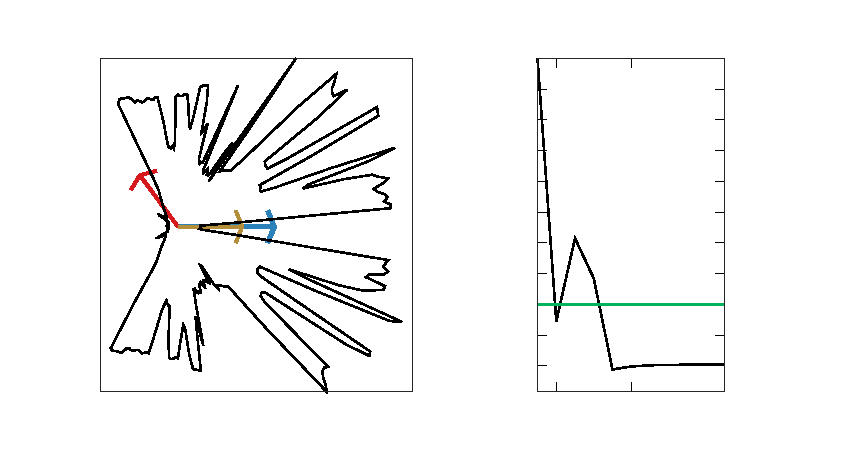
\includegraphics{./figures/parts/02/chapters/04/sections/02/rc_x1}}%
    \gplfronttext
  \end{picture}%
\endgroup

  \vspace{0.5cm}
  \caption{\small Αριστερά: η αρχική
           $\hat{\bm{p}}[0] \equiv (\bm{l},\hat{\theta}[0])$ και τελική
           $\hat{\bm{p}}[1] \equiv (\bm{l},\hat{\theta}[1])$ εκτίμηση στάσης του
           αισθητήρα σε ένα περιβάλλον με χάρτη $\bm{M}$, για πραγματική στάση
           $\bm{p}(\bm{l},\theta)$, ως συνέπεια της εφαρμογής της μεθόδου
           γωνιακής ευθυγράμμισης Πρώτων Αρχών. Δεξιά: το σφάλμα εκτίμησης
           προσανατολισμού ως συνάρτηση της διακριτικής γωνίας $\gamma$ του
           αισθητήρα}
  \label{fig:02_04_02:rc_x1}
\end{figure}

\begin{algorithm}[h]
  \caption{\texttt{rc\_x1}}
  \begin{spacing}{1.3}
  \begin{algorithmic}[1]
    \REQUIRE $\mathcal{S}_R$, $\mathcal{S}_V$, $\hat{\bm{p}}(x, y, \hat{\theta})$
    \ENSURE $\hat{\theta}^\prime$
    %\STATE $\mathcal{S}_V \leftarrow \texttt{scan\_map}(\bm{M}, \hat{\bm{p}}, N_s)$
    \STATE $\bm{R} = \mathcal{F}\{\mathcal{S}_R\}[1]$
    \STATE $\bm{V} = \mathcal{F}\{\mathcal{S}_V\}[1]$
    \STATE $\hat{\theta}^\prime \leftarrow \hat{\theta} + \arg(\bm{R}) - \arg(\bm{V})$
    \RETURN $\hat{\theta}^\prime$
  \end{algorithmic}
  \end{spacing}
  \label{alg:algorithm_x1rc}
\end{algorithm}

%%%%%%%%%%%%%%%%%%%%%%%%%%%%%%%%%%%%%%%%%%%%%%%%%%%%%%%%%%%%%%%%%%%%%%%%%%%%%%%%
\subsection{Η μέθοδος του Προκρούστη}
\label{subsection:02_04_02:03}

Έστω ότι η προβολή των τελικών σημείων των ακτίνων της σάρωσης $\mathcal{S}_V$
γύρω από τη στάση $\hat{\bm{p}}(x,y,\hat{\theta})$ παράγει το σύνολο σημείων
$\bm{P}_V$ στο οριζόντιο επίπεδο. Έστω ότι η ίδια προβολή για τη σάρωση
$\mathcal{S}_R$ ως προς τη στάση $\bm{p}(x,y,\theta)$ παράγει το σύνολο
$\bm{P}_R$. Η περιστροφή της στάσης $\hat{\bm{p}}$ που ευθυγραμμίζει βέλτιστα
το σύνολο σημείων $\bm{P}_V$ σε σχέση με το $\bm{P}_R$ μπορεί να βρεθεί από τη
λύση του Ορθογώνιου Προσκρούστειου προβλήματος \cite{Schonemann1966a} για
πίνακες εισόδου $\bm{P}_V$ και $\bm{P}_R$. Στην περίπτωση που ο πίνακας
μετασχηματισμού περιορίζεται στο να έχει τη δομή πίνακα περιστροφής $\bm{R}$:
$\det{(\bm{R})} = 1$, το πρόβλημα ευθυγράμμισης ονομάζεται Περιορισμένο
Ορθογώνιο Προσκρούστειο πρόβλημα.

Σε αυτή την ενότητα αναζητούμε την λύση αυτού του τελευταίου προβλήματος ως
μέσο επίλυσης του προβλήματος \ref{}, διότι ο περιορισμός του πίνακα
μετασχηματισμού σε πίνακα περιστροφής δίνει τη δυνατότητα προσδιορισμού της
γωνίας περιστροφής της εκτίμησης στάσης από την οποία το εικονικό διάνυσμα
σαρώσεων εμφανίζει τη βέλτιστη ευθυγράμμιση με το πραγματικό διάνυσμα
$\mathcal{S}_R$. Η λύση του Περιορισμένου Ορθογώνιου Προσκρούστειου προβλήματος
δίνεται στο \cite{Umeyama1991} και περιγράφεται παρακάτω.

Δεδομένου ότι στα συμφραζόμενα του προβλήματός \ref{prob:02_04} η θέση $\bm{l}$
είναι άγνωστη, τα τελικά σημεία κάθε σάρωσης λαμβάνονται με την προβολή κάθε
σάρωσης στο επίπεδο $x-y$ σύμφωνα με το τοπικό σύστημα αναφοράς της κάθεμίας,
δηλαδή σαν να είχε ληφθεί η κάθε μιά από το $O(0,0,0)$. Ο πίνακας περιστροφής
$\bm{R}$ που ευθυγραμμίζει βέλτιστα το σύνολο $\bm{P}_V$ με το $\bm{P}_R$ είναι
ο πίνακας που ελαχιστοποιεί την απόκλιση των περιεστραμμένων σημείων
$\bm{R}\bm{P}_V$ από το $\bm{P}_R$:
\begin{align}
  \operatorname*{arg\,min}\limits_{\bm{R}} \|\bm{P}_R - \bm{R} \cdot \bm{P}_V\|_F^2 \nonumber
\end{align}
όπου $\|\bm{A}\|_F = (\bm{A}^\top\bm{A})^{1/2}$ δηλώνει το μέτρο Frobenius του
πίνακα πραγματικών τιμών $\bm{A}$. Έστω ο τελεστής $\text{tr}(\bm{A})$ ότι
δηλώνει το ίχνος του πίνακα $\bm{A}$. Τότε
\begin{align}
  \|\bm{P}_R - \bm{R} \bm{P}_V\|_F^2 = \text{tr}(\bm{P}_R^\top \bm{P}_R + \bm{P}_V^\top \bm{P}_V) - 2 \ \text{tr}(\bm{R} \bm{P}_R \bm{P}_V^\top)
  \label{eq:expanded_frob_norm}
\end{align}

Δεδομένου ότι μόνο ο δεύτερος όρος της δεξιάς πλευράς εξαρτάται από τον πίνακα
$\bm{R}$, για την ελαχιστοποίηση της (\ref{eq:expanded_frob_norm}) ως προς
$\bm{R}$ αρκεί να βρεθεί ο πίνακας περιστροφής $\bm{R}$ που μεγιστοποιεί
το ίχνος $\text{tr}(\bm{R} \bm{P}_V \bm{P}_R^\top)$. Ο βέλτιστος πίνακας
$\bm{R}$ δίνεται από το Λήμμα \ref{lm:umeyama}:

\begin{lemma}
  \label{lm:umeyama}
  Έστω $\bm{P}_R$ και $\bm{P}_V$ πίνακες διαστάσεων $2 \times N_s$, $\bm{R}$
  πίνακας διαστάσεων $2 \times 2$, και $\bm{U} \bm{D} \bm{V}^\top$ η αποσύνθεση
  του $\bm{P}_R \bm{P}_V^\top$ σε ιδιάζουσες τιμές (Singular Value
  Decomposition---SVD). Τότε ο πίνακας $\bm{R}$ που ελαχιστοποιεί το μέτρο
  $\|\bm{P}_R - \bm{R} \cdot \bm{P}_V\|_F^2$ δίνεται από τη σχέση
  $\bm{R} = \bm{U} \bm{S} \bm{V}^\top$, όπου
  $\bm{S} = \text{diag}(1,\det{(\bm{U}\bm{V})})$.
\end{lemma}

\begin{corollary}
  \label{corollary:umeyama}
  Η τιμή του μέγιστου ίχνους
  $T(\bm{P}_R, \bm{P}_V) \triangleq \max\text{tr}(\bm{R} \bm{P}_R \bm{P}_V^\top)$
  είναι
  \begin{align}
  \max\text{tr}(\bm{R} \bm{P}_R \bm{P}_V^\top) = \text{tr}(\bm{D}\bm{S})
  \end{align}
\end{corollary}

Το Λήμμα \ref{lm:umeyama} παρέχει τον βέλτιστο πίνακα περιστροφής $\bm{R}$ υπό
την προϋπόθεση ότι τόσο το σύνολο $\bm{P}_R$ όσο και το $\bm{P}_V$ είναι
γνωστά.  Ωστόσο, στα συμφραζόμενα του προβλήματος \ref{prob:02_04} τα τελικά
σημεία $\bm{P}_R$ υπολογίζονται από έναν αυθαίρετο προσανατολισμό επειδή ο
επιθυμητός προσανατολισμός είναι θεμελιωδώς άγνωστος. Επομένως ο υπολογισμός
του πίνακα $\bm{R}$ και η εξαγωγή  του σχετικού προσανατολισμού του $\bm{P}_V$
σε σχέση με το $\bm{P}_R$ από τον πίνακα $\bm{R}$ \textit{σε ένα βήμα} είναι
αδύνατη. Αυτό που μπορεί να γίνει για την εκτίμηση του προσανατολισμού της
στάσης $\bm{p}$ ως προς τον προσανατολισμό της στάσης $\hat{\bm{p}}$ είναι το
εξής. Υπολογίζεται το γινόμενο $\bm{P}_R \bm{P}_V^\top$ σε $O(N_s^2)$, η
αποσύνθεσή του σε ιδιάζουσες τιμές σε $O(1)$, καταγράφεται η τιμή του ίχνους
$\text{tr}(\bm{D}\bm{S})$ σε $O(1)$, μετατοπίζεται ο πίνακας $\bm{P}_V$ κατά
στήλες προς τα αριστερά μία φορά, και επαναλαμβάνεται η διαδικασία $N_s-1$
φορές. Έστω ότι η επανάληψη $\psi \in \mathbb{Z}_{\geq 0}$ καταγράφει το
μέγιστο ίχνος: τότε η περιστροφή της στάσης $\hat{\bm{p}}$ κατά $\psi \gamma$
μεγιστοποιεί το ίχνος $\text{tr}(\bm{R} \bm{P}_R \bm{P}_V^\top)$ και
ελαχιστοποιεί το μέτρο του σφάλματος ευθυγράμμισης
(\ref{eq:expanded_frob_norm}) για μία δεδομένη διακριτική γωνία $\gamma$. Η
παραπάνω διαδικασία αποδίδει τη βέλτιστη περιστροφή επειδή το ίχνος
$\text{tr}(\bm{D}\bm{S})$ ουσιαστικά αναλαμβάνει το ρόλο ενός μέτρου
ευθυγράμμισης μεταξύ των συνόλων σημείων $\bm{P}_V$ και $\bm{P}_R$.

Η παραπάνω διαδικασία καταγραφής $N_s$ ιχνών μπορεί να υπολογιστεί είτε με ευθύ
τρόπο, πολυπλοκότητας $O(N_s^3)$, είτε μέσω με της μεθόδου που παρουσιάζεται
στο \cite{Dogan2015} με σημαντικά μειωμένη πολυπλοκότητα $O(N_s \log N_s)$.  Η
μέθοδος αυτή θα αναφέρεται στο εξής ως μέθοδος DBH και περιγράφεται παρακάτω.


Έστω $\widetilde{\bm{A}}$ ο πίνακας $\bm{A}$ με αντίστροφη σειρά στηλών,
$\bm{P}_R = [\bm{p}_R^x; \bm{p}_R^y]$,
$\widetilde{\bm{P}}_V = [\bm{p}_V^x; \bm{p}_V^y]$. Έστω επίσης ότι ο τελεστής
$\odot$ υποδηλώνει τον πολλαπλασιασμό κατά στοιχείο. Τότε υπολογίζονται
τέσσερα διανύσματα μεγέθους $N_s$:
\begin{align}
  \bm{m}_{11} = \mathcal{F}^{-1}\{ \mathcal{F}\{\bm{p}_R^x\} \odot \mathcal{F}\{\bm{p}_V^x\} \} \} \nonumber \\
  \bm{m}_{12} = \mathcal{F}^{-1}\{ \mathcal{F}\{\bm{p}_R^y\} \odot \mathcal{F}\{\bm{p}_V^x\} \} \} \nonumber \\
  \bm{m}_{21} = \mathcal{F}^{-1}\{ \mathcal{F}\{\bm{p}_R^x\} \odot \mathcal{F}\{\bm{p}_V^y\} \} \} \nonumber \\
  \bm{m}_{22} = \mathcal{F}^{-1}\{ \mathcal{F}\{\bm{p}_R^y\} \odot \mathcal{F}\{\bm{p}_V^y\} \} \} \nonumber
\end{align}
Μετά τον υπολογισμό των διανυσμάτων $\bm{m}_{kl}$, $k,l = 1,2$, υπολογίζονται
$N_s$ πίνακες $\bm{M}_j$, μεγέθους $2\times2$, σύμφωνα με:
\begin{align}
  \bm{M}_j =
  \begin{bmatrix}
    \bm{m}_{11}^j & \bm{m}_{12}^j \\
    \bm{m}_{21}^j & \bm{m}_{22}^j
  \end{bmatrix}
\end{align}
όπου $j = 0,\dots,N-1$, και $\bm{m}_{kl}^j$ είναι το $j$-οστό στοιχείο του
διανύσματος $\bm{m}_{kl}$. Ο πίνακας $\bm{M}_j$ είναι ίσος με τον πίνακα
$\bm{P}_R (\bm{P}_V^{N_s-1-j})^\top$, όπου ο συμβολισμός $\bm{A}^k$  δηλώνει
τον πίνακα $\bm{A}$ του οποίου οι στήλες έχουν μετατοπιστεί $k$ φορές προς τα
αριστερά. Η απόδειξη χρησιμοποιεί το Θεώρημα Κυκλικής Συνέλιξης του DFT και
παραλείπεται.

Αφού υπολογιστούν και σχηματιστούν όλοι οι $N_s$ $\bm{M}_j$ πίνακες, κάθε ένας
αποσυντίθεται σε ιδιάζουσες τιμές. Το ίχνος κάθε πίνακα $\bm{R}_j \bm{M}_j$
καταγράφεται με την εφαρμογή του Λήμματος \ref{lm:umeyama} και του Επακόλουθου
\ref{corollary:umeyama}. Έστω ότι το μέγιστο ίχνος καταγράφεται για τον δείκτη
$J$, τότε η περιστροφή της στάσης $\hat{\bm{p}}$ κατά $(N_s-1-J)\gamma =
\psi\gamma$ επιτυγχάνει το ίδιο αποτέλεσμα με την ευθεία μέθοδο υψηλότερης
πολυπλοκότητας για μία δεδομένη διακριτική γωνία $\gamma$. Εάν η διαφορά του
προσανατολισμού μεταξύ των στάσεων από τις οποίες ελήφθησαν οι σαρώσεις
$\mathcal{S}_R$ και $\mathcal{S}_V$ είναι $\Delta\theta = \theta-\hat{\theta}$,
τότε $\Delta\theta = (N_s-1-J)\gamma + \phi$, όπου
$\mod(\Delta\theta, \gamma) = \phi \in [-\dfrac{\gamma}{2},+\dfrac{\gamma}{2}]$.
Τα παραπάνω μας οδηγούν στη διατύπωση του Λήμματος \ref{lemma:02_04_02:03}:

\begin{lemma}
  Έστω οι παραδοχές του προβλήματος \ref{prob:02_04} και $\hat{\bm{l}} = \bm{l}$.
  Έστω επίσης ότι (α) οι μετρήσεις του φυσικού αισθητήρα δεν φέρουν
  διαταραχές, και (β) ο χάρτης $\bm{M}$ αναπαριστά το περιβάλλον τέλεια. Τότε
  ενημερώνοντας την εκτίμηση προσανατολισμού σε
  $\hat{\theta}^\prime$:
  \begin{align}
    \hat{\theta}^\prime = \hat{\theta} + \psi \gamma \label{eq:update_t3}
  \end{align}
  όπου $\psi$ δίνεται από τη γραμμή 5 του Αλγορίθμου \ref{alg:algorithm_ufrc},
  οδηγεί σε ένα επίλοιπο σφάλμα προσανατολισμού $\phi$:
  \begin{align}
    |\phi| \leq \dfrac{\gamma}{2}  \label{eq:phi_3}
  \end{align}
  \label{lemma:02_04_02:03}
\end{lemma}

\begin{corollary}
  Ο στόχος (\ref{objective:02_04}) επιτυγχάνεται υπό την προϋπόθεση ότι
  $|\theta-\hat{\theta}| > \dfrac{\gamma}{2}$.
\end{corollary}

Η παραπάνω μέθοδος εκτίμησης του προσανατολισμού της στάσης $\bm{p}(x,y,\theta)$
ονομάζεται στο εξής μέθοδος του Προκρούστη. Στο σχήμα
\ref{fig:02_04_02:ku_vs_dbh} απεικονίζεται το κέρδος της εφαρμογής της μεθόδου
DBH έναντι της αφελούς μεθόδου σε χρόνο εκτέλεσης για αύξοντες αριθμούς
εκπεμπόμενων από τον αισθητήρα σάρωσης ακτίνων $N_s$.

\begin{figure}[h]\centering
  \vspace{1.0cm}
  \definecolor{k}{RGB}{0,0,0}
\definecolor{g}{RGB}{200,200,200}
% GNUPLOT: LaTeX picture with Postscript
\begingroup
  \makeatletter
  \providecommand\color[2][]{%
    \GenericError{(gnuplot) \space\space\space\@spaces}{%
      Package color not loaded in conjunction with
      terminal option `colourtext'%
    }{See the gnuplot documentation for explanation.%
    }{Either use 'blacktext' in gnuplot or load the package
      color.sty in LaTeX.}%
    \renewcommand\color[2][]{}%
  }%
  \providecommand\includegraphics[2][]{%
    \GenericError{(gnuplot) \space\space\space\@spaces}{%
      Package graphicx or graphics not loaded%
    }{See the gnuplot documentation for explanation.%
    }{The gnuplot epslatex terminal needs graphicx.sty or graphics.sty.}%
    \renewcommand\includegraphics[2][]{}%
  }%
  \providecommand\rotatebox[2]{#2}%
  \@ifundefined{ifGPcolor}{%
    \newif\ifGPcolor
    \GPcolorfalse
  }{}%
  \@ifundefined{ifGPblacktext}{%
    \newif\ifGPblacktext
    \GPblacktexttrue
  }{}%
  % define a \g@addto@macro without @ in the name:
  \let\gplgaddtomacro\g@addto@macro
  % define empty templates for all commands taking text:
  \gdef\gplbacktext{}%
  \gdef\gplfronttext{}%
  \makeatother
  \ifGPblacktext
    % no textcolor at all
    \def\colorrgb#1{}%
    \def\colorgray#1{}%
  \else
    % gray or color?
    \ifGPcolor
      \def\colorrgb#1{\color[rgb]{#1}}%
      \def\colorgray#1{\color[gray]{#1}}%
      \expandafter\def\csname LTw\endcsname{\color{white}}%
      \expandafter\def\csname LTb\endcsname{\color{black}}%
      \expandafter\def\csname LTa\endcsname{\color{black}}%
      \expandafter\def\csname LT0\endcsname{\color[rgb]{1,0,0}}%
      \expandafter\def\csname LT1\endcsname{\color[rgb]{0,1,0}}%
      \expandafter\def\csname LT2\endcsname{\color[rgb]{0,0,1}}%
      \expandafter\def\csname LT3\endcsname{\color[rgb]{1,0,1}}%
      \expandafter\def\csname LT4\endcsname{\color[rgb]{0,1,1}}%
      \expandafter\def\csname LT5\endcsname{\color[rgb]{1,1,0}}%
      \expandafter\def\csname LT6\endcsname{\color[rgb]{0,0,0}}%
      \expandafter\def\csname LT7\endcsname{\color[rgb]{1,0.3,0}}%
      \expandafter\def\csname LT8\endcsname{\color[rgb]{0.5,0.5,0.5}}%
    \else
      % gray
      \def\colorrgb#1{\color{black}}%
      \def\colorgray#1{\color[gray]{#1}}%
      \expandafter\def\csname LTw\endcsname{\color{white}}%
      \expandafter\def\csname LTb\endcsname{\color{black}}%
      \expandafter\def\csname LTa\endcsname{\color{black}}%
      \expandafter\def\csname LT0\endcsname{\color{black}}%
      \expandafter\def\csname LT1\endcsname{\color{black}}%
      \expandafter\def\csname LT2\endcsname{\color{black}}%
      \expandafter\def\csname LT3\endcsname{\color{black}}%
      \expandafter\def\csname LT4\endcsname{\color{black}}%
      \expandafter\def\csname LT5\endcsname{\color{black}}%
      \expandafter\def\csname LT6\endcsname{\color{black}}%
      \expandafter\def\csname LT7\endcsname{\color{black}}%
      \expandafter\def\csname LT8\endcsname{\color{black}}%
    \fi
  \fi
    \setlength{\unitlength}{0.0500bp}%
    \ifx\gptboxheight\undefined%
      \newlength{\gptboxheight}%
      \newlength{\gptboxwidth}%
      \newsavebox{\gptboxtext}%
    \fi%
    \setlength{\fboxrule}{0.5pt}%
    \setlength{\fboxsep}{1pt}%
\begin{picture}(4000.00,3000.00)%
    \gplgaddtomacro\gplbacktext{%
      \colorrgb{0.00,0.00,0.00}%
      \put(468,330){\makebox(0,0)[r]{\strut{}$0.3$}}%
      \colorrgb{0.00,0.00,0.00}%
      \put(468,1308){\makebox(0,0)[r]{\strut{}$0.4$}}%
      \colorrgb{0.00,0.00,0.00}%
      \put(468,2285){\makebox(0,0)[r]{\strut{}$0.5$}}%
      \colorrgb{0.15,0.15,0.15}%
      \put(600,110){\makebox(0,0){\strut{}$0$}}%
      \colorrgb{0.15,0.15,0.15}%
      \put(1606,110){\makebox(0,0){\strut{}$1$}}%
      \colorrgb{0.15,0.15,0.15}%
      \put(2613,110){\makebox(0,0){\strut{}$2$}}%
      \colorrgb{0.15,0.15,0.15}%
      \put(3619,110){\makebox(0,0){\strut{}$3$}}%
    }%
    \gplgaddtomacro\gplfronttext{%
      \colorrgb{0.00,0.00,0.00}%
      \put(1209,3194){\makebox(0,0){\strut{}{\color{k}{\rule[0.6mm]{0.5cm}{0.5mm}}} $\dfrac{T_{\texttt{DBH}}}{T_{\text{naive}}}$}}%
      \put(2809,3194){\makebox(0,0){\strut{}{\color{g}{\rule[0.6mm]{0.5cm}{0.5mm}}} $\dfrac{N \log(N)}{N^3}$}}%
      \put(2109,-220){\makebox(0,0){\strut{}Βαθμός δειγματολειψίας $\nu$}}%
    }%
    \gplgaddtomacro\gplbacktext{%
      \colorrgb{0.00,0.00,0.00}%
      \put(3751,330){\makebox(0,0)[l]{\strut{}}}%
      \colorrgb{0.00,0.00,0.00}%
      \put(3751,819){\makebox(0,0)[l]{\strut{}}}%
      \colorrgb{0.00,0.00,0.00}%
      \put(3751,1308){\makebox(0,0)[l]{\strut{}}}%
      \colorrgb{0.00,0.00,0.00}%
      \put(3751,1796){\makebox(0,0)[l]{\strut{}}}%
      \colorrgb{0.00,0.00,0.00}%
      \put(3751,2285){\makebox(0,0)[l]{\strut{}}}%
      \colorrgb{0.00,0.00,0.00}%
      \put(3751,2774){\makebox(0,0)[l]{\strut{}}}%
    }%
    \gplgaddtomacro\gplfronttext{%
    }%
    \gplbacktext
    \put(0,0){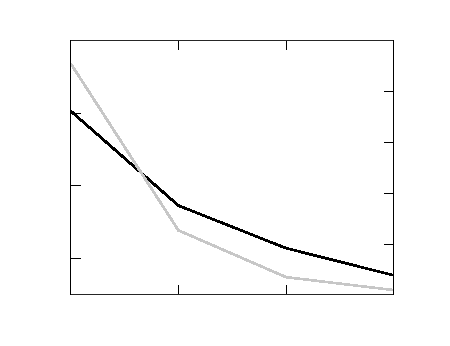
\includegraphics{./figures/parts/02/chapters/04/sections/02/ku_vs_dbh}}%
    \gplfronttext
  \end{picture}%
\endgroup

  \vspace{0.5cm}
  \caption{\small Το ποσοστό του χρόνου εκτέλεσης της μεθόδου ευθυγράμμισης
           Προκρούστη με την εφαρμογή της μεθόδου DBH προς το χρόνο εκτέλεσης
           χωρίς την εφαρμογή της, για αυξανόμενο αριθμό εκπεμπόμενων ακτίνων
           του αισθητήρα σάρωσης}
  \label{fig:02_04_02:ku_vs_dbh}
\end{figure}

Στο σχήμα \ref{fig:02_04_02:rc_uf} απεικονίζεται η αρχική και τελική συνθήκη
ευθυγράμμισης προσανατολισμού με εφαρμογή της μεθόδου Προκρούστη για έναν
αισθητήρα δισδιάστατων πανοραμικών σαρώσεων με $\gamma = 2\pi/360$, σε ένα μη
δομημένο περιβάλλον, του οποίου ο χάρτης το αναπαριστά τέλεια, ενώ οι μετρήσεις
του αισθητήρα δεν διαταράσσονται από θόρυβο. Το σχήμα
\ref{fig:02_04_02:rc_uf_exec_time} απεικονίζει το μέσο χρόνο εκτέλεσης
μίας επανάληψης της μεθόδου σε δέκα εκτελέσεις για αυξανόμενο μέγεθος σαρώσεων
$N_s$. Ο Αλγόριθμος \ref{alg:algorithm_x1rc} παρουσιάζει σε ψευδοκώδικα τη
διαδικασία διόρθωσης προσανατολισμού με βάση την εν λόγω μέθοδο. Ο Αλγόριθμος
\ref{alg:algorithm_core_ufrc} παρουσιάζει σε ψευδοκώδικα τη μέθοδο DBH.

\begin{figure}[h]\centering
  % GNUPLOT: LaTeX picture with Postscript
\begingroup
  \makeatletter
  \providecommand\color[2][]{%
    \GenericError{(gnuplot) \space\space\space\@spaces}{%
      Package color not loaded in conjunction with
      terminal option `colourtext'%
    }{See the gnuplot documentation for explanation.%
    }{Either use 'blacktext' in gnuplot or load the package
      color.sty in LaTeX.}%
    \renewcommand\color[2][]{}%
  }%
  \providecommand\includegraphics[2][]{%
    \GenericError{(gnuplot) \space\space\space\@spaces}{%
      Package graphicx or graphics not loaded%
    }{See the gnuplot documentation for explanation.%
    }{The gnuplot epslatex terminal needs graphicx.sty or graphics.sty.}%
    \renewcommand\includegraphics[2][]{}%
  }%
  \providecommand\rotatebox[2]{#2}%
  \@ifundefined{ifGPcolor}{%
    \newif\ifGPcolor
    \GPcolorfalse
  }{}%
  \@ifundefined{ifGPblacktext}{%
    \newif\ifGPblacktext
    \GPblacktexttrue
  }{}%
  % define a \g@addto@macro without @ in the name:
  \let\gplgaddtomacro\g@addto@macro
  % define empty templates for all commands taking text:
  \gdef\gplfronttext{}%
  \gdef\gplfronttext{}%
  \makeatother
  \ifGPblacktext
    % no textcolor at all
    \def\colorrgb#1{}%
    \def\colorgray#1{}%
  \else
    % gray or color?
    \ifGPcolor
      \def\colorrgb#1{\color[rgb]{#1}}%
      \def\colorgray#1{\color[gray]{#1}}%
      \expandafter\def\csname LTw\endcsname{\color{white}}%
      \expandafter\def\csname LTb\endcsname{\color{black}}%
      \expandafter\def\csname LTa\endcsname{\color{black}}%
      \expandafter\def\csname LT0\endcsname{\color[rgb]{1,0,0}}%
      \expandafter\def\csname LT1\endcsname{\color[rgb]{0,1,0}}%
      \expandafter\def\csname LT2\endcsname{\color[rgb]{0,0,1}}%
      \expandafter\def\csname LT3\endcsname{\color[rgb]{1,0,1}}%
      \expandafter\def\csname LT4\endcsname{\color[rgb]{0,1,1}}%
      \expandafter\def\csname LT5\endcsname{\color[rgb]{1,1,0}}%
      \expandafter\def\csname LT6\endcsname{\color[rgb]{0,0,0}}%
      \expandafter\def\csname LT7\endcsname{\color[rgb]{1,0.3,0}}%
      \expandafter\def\csname LT8\endcsname{\color[rgb]{0.5,0.5,0.5}}%
    \else
      % gray
      \def\colorrgb#1{\color{black}}%
      \def\colorgray#1{\color[gray]{#1}}%
      \expandafter\def\csname LTw\endcsname{\color{white}}%
      \expandafter\def\csname LTb\endcsname{\color{black}}%
      \expandafter\def\csname LTa\endcsname{\color{black}}%
      \expandafter\def\csname LT0\endcsname{\color{black}}%
      \expandafter\def\csname LT1\endcsname{\color{black}}%
      \expandafter\def\csname LT2\endcsname{\color{black}}%
      \expandafter\def\csname LT3\endcsname{\color{black}}%
      \expandafter\def\csname LT4\endcsname{\color{black}}%
      \expandafter\def\csname LT5\endcsname{\color{black}}%
      \expandafter\def\csname LT6\endcsname{\color{black}}%
      \expandafter\def\csname LT7\endcsname{\color{black}}%
      \expandafter\def\csname LT8\endcsname{\color{black}}%
    \fi
  \fi
    \setlength{\unitlength}{0.0500bp}%
    \ifx\gptboxheight\undefined%
      \newlength{\gptboxheight}%
      \newlength{\gptboxwidth}%
      \newsavebox{\gptboxtext}%
    \fi%
    \setlength{\fboxrule}{0.5pt}%
    \setlength{\fboxsep}{1pt}%
\begin{picture}(4800.00,3600.00)%
    \gplgaddtomacro\gplfronttext{%
      \colorrgb{0.15,0.15,0.15}%
      \put(814,704){\makebox(0,0)[r]{\strut{}$0.0$}}%
      \colorrgb{0.15,0.15,0.15}%
      \put(814,1175){\makebox(0,0)[r]{\strut{}$1.0$}}%
      \colorrgb{0.15,0.15,0.15}%
      \put(814,1646){\makebox(0,0)[r]{\strut{}$2.0$}}%
      \colorrgb{0.15,0.15,0.15}%
      \put(814,2117){\makebox(0,0)[r]{\strut{}$3.0$}}%
      \colorrgb{0.15,0.15,0.15}%
      \put(814,2588){\makebox(0,0)[r]{\strut{}$4.0$}}%
      \colorrgb{0.15,0.15,0.15}%
      \put(814,3059){\makebox(0,0)[r]{\strut{}$5.0$}}%
      \colorrgb{0.15,0.15,0.15}%
      \put(946,484){\makebox(0,0){\strut{}$360$$\cdot$$2^0$}}%
      \colorrgb{0.15,0.15,0.15}%
      \put(2055,484){\makebox(0,0){\strut{}$360$$\cdot$$2^1$}}%
      \colorrgb{0.15,0.15,0.15}%
      \put(3163,484){\makebox(0,0){\strut{}$360$$\cdot$$2^2$}}%
      \colorrgb{0.15,0.15,0.15}%
      \put(4272,484){\makebox(0,0){\strut{}$360$$\cdot$$2^3$}}%
    }%
    \gplgaddtomacro\gplfronttext{%
      \colorrgb{0.15,0.15,0.15}%
      \put(176,1881){\rotatebox{90}{\makebox(0,0){\strut{}Χρόνος εκτέλεσης [ms]}}}%
      \colorrgb{0.15,0.15,0.15}%
      \put(2609,154){\makebox(0,0){\strut{}Αριθμός ακτίνων $N_s$}}%
      \colorrgb{0.00,0.00,0.00}%
      \put(2609,3269){\makebox(0,0){\strut{}$T_{\texttt{rc\_uf}}$}}%
    }%
    \put(0,0){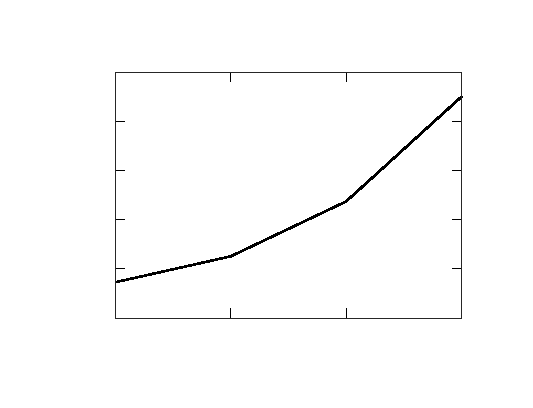
\includegraphics{./figures/parts/02/chapters/04/sections/02/times_rc_uf}}%
    \gplfronttext
  \end{picture}%
\endgroup

  \caption{\small Ο μέσος χρόνος εκτέλεσης μίας επανάληψης της μεθόδου
           Προκρούστη διάστασης για δέκα εκτελέσεις, ανά μέγεθος σαρώσεων εισόδου
           $N_s$}
  \label{fig:02_04_02:rc_uf_exec_time}
\end{figure}

\begin{figure}[h]\centering
  \vspace{0.5cm}
  \definecolor{sr}{RGB}{43,131,186}
\definecolor{svi}{RGB}{215,25, 28}
\definecolor{svf}{RGB}{179,143,59}
\definecolor{g}{RGB}{0,178,93}
\definecolor{k}{RGB}{0,0,0}

% GNUPLOT: LaTeX picture with Postscript
\begingroup
  \makeatletter
  \providecommand\color[2][]{%
    \GenericError{(gnuplot) \space\space\space\@spaces}{%
      Package color not loaded in conjunction with
      terminal option `colourtext'%
    }{See the gnuplot documentation for explanation.%
    }{Either use 'blacktext' in gnuplot or load the package
      color.sty in LaTeX.}%
    \renewcommand\color[2][]{}%
  }%
  \providecommand\includegraphics[2][]{%
    \GenericError{(gnuplot) \space\space\space\@spaces}{%
      Package graphicx or graphics not loaded%
    }{See the gnuplot documentation for explanation.%
    }{The gnuplot epslatex terminal needs graphicx.sty or graphics.sty.}%
    \renewcommand\includegraphics[2][]{}%
  }%
  \providecommand\rotatebox[2]{#2}%
  \@ifundefined{ifGPcolor}{%
    \newif\ifGPcolor
    \GPcolorfalse
  }{}%
  \@ifundefined{ifGPblacktext}{%
    \newif\ifGPblacktext
    \GPblacktexttrue
  }{}%
  % define a \g@addto@macro without @ in the name:
  \let\gplgaddtomacro\g@addto@macro
  % define empty templates for all commands taking text:
  \gdef\gplfronttext{}%
  \gdef\gplfronttext{}%
  \makeatother
  \ifGPblacktext
    % no textcolor at all
    \def\colorrgb#1{}%
    \def\colorgray#1{}%
  \else
    % gray or color?
    \ifGPcolor
      \def\colorrgb#1{\color[rgb]{#1}}%
      \def\colorgray#1{\color[gray]{#1}}%
      \expandafter\def\csname LTw\endcsname{\color{white}}%
      \expandafter\def\csname LTb\endcsname{\color{black}}%
      \expandafter\def\csname LTa\endcsname{\color{black}}%
      \expandafter\def\csname LT0\endcsname{\color[rgb]{1,0,0}}%
      \expandafter\def\csname LT1\endcsname{\color[rgb]{0,1,0}}%
      \expandafter\def\csname LT2\endcsname{\color[rgb]{0,0,1}}%
      \expandafter\def\csname LT3\endcsname{\color[rgb]{1,0,1}}%
      \expandafter\def\csname LT4\endcsname{\color[rgb]{0,1,1}}%
      \expandafter\def\csname LT5\endcsname{\color[rgb]{1,1,0}}%
      \expandafter\def\csname LT6\endcsname{\color[rgb]{0,0,0}}%
      \expandafter\def\csname LT7\endcsname{\color[rgb]{1,0.3,0}}%
      \expandafter\def\csname LT8\endcsname{\color[rgb]{0.5,0.5,0.5}}%
    \else
      % gray
      \def\colorrgb#1{\color{black}}%
      \def\colorgray#1{\color[gray]{#1}}%
      \expandafter\def\csname LTw\endcsname{\color{white}}%
      \expandafter\def\csname LTb\endcsname{\color{black}}%
      \expandafter\def\csname LTa\endcsname{\color{black}}%
      \expandafter\def\csname LT0\endcsname{\color{black}}%
      \expandafter\def\csname LT1\endcsname{\color{black}}%
      \expandafter\def\csname LT2\endcsname{\color{black}}%
      \expandafter\def\csname LT3\endcsname{\color{black}}%
      \expandafter\def\csname LT4\endcsname{\color{black}}%
      \expandafter\def\csname LT5\endcsname{\color{black}}%
      \expandafter\def\csname LT6\endcsname{\color{black}}%
      \expandafter\def\csname LT7\endcsname{\color{black}}%
      \expandafter\def\csname LT8\endcsname{\color{black}}%
    \fi
  \fi
    \setlength{\unitlength}{0.0500bp}%
    \ifx\gptboxheight\undefined%
      \newlength{\gptboxheight}%
      \newlength{\gptboxwidth}%
      \newsavebox{\gptboxtext}%
    \fi%
    \setlength{\fboxrule}{0.5pt}%
    \setlength{\fboxsep}{1pt}%
\begin{picture}(8000.00,4000.00)%
    \gplgaddtomacro\gplfronttext{%
    }%
    \gplgaddtomacro\gplfronttext{%
    }%
    \gplgaddtomacro\gplfronttext{%
      \colorrgb{0.15,0.15,0.15}%
      \put(4868,400){\makebox(0,0)[r]{\strut{}$2^{-2}$}}%
      \colorrgb{0.15,0.15,0.15}%
      \put(4868,755){\makebox(0,0)[r]{\strut{}$2^{-1}$}}%
      \colorrgb{0.15,0.15,0.15}%
      \put(4868,1111){\makebox(0,0)[r]{\strut{}$2^{0}$}}%
      \colorrgb{0.15,0.15,0.15}%
      \put(4868,1466){\makebox(0,0)[r]{\strut{}$2^{1}$}}%
      \colorrgb{0.15,0.15,0.15}%
      \put(4868,1822){\makebox(0,0)[r]{\strut{}$2^{2}$}}%
      \colorrgb{0.15,0.15,0.15}%
      \put(4868,2177){\makebox(0,0)[r]{\strut{}$2^{3}$}}%
      \colorrgb{0.15,0.15,0.15}%
      \put(4868,2533){\makebox(0,0)[r]{\strut{}$2^{4}$}}%
      \colorrgb{0.15,0.15,0.15}%
      \put(4868,2888){\makebox(0,0)[r]{\strut{}$2^{5}$}}%
      \colorrgb{0.15,0.15,0.15}%
      \put(4868,3244){\makebox(0,0)[r]{\strut{}$2^{6}$}}%
      \colorrgb{0.15,0.15,0.15}%
      \put(4868,3599){\makebox(0,0)[r]{\strut{}$2^{7}$}}%
      \colorrgb{0.15,0.15,0.15}%
      \put(5180,180){\makebox(0,0){\strut{}$1$}}%
      \colorrgb{0.15,0.15,0.15}%
      \put(5900,180){\makebox(0,0){\strut{}$5$}}%
      \colorrgb{0.15,0.15,0.15}%
      \put(6799,180){\makebox(0,0){\strut{}$10$}}%
    }%
    \gplgaddtomacro\gplfronttext{%
      \colorrgb{0.00,0.00,0.00}%
      \put(5400,3919){\makebox(0,0){\strut{}{\color{k}{\rule[0.6mm]{0.5cm}{0.5mm}}} $\dfrac{|\theta-\hat{\theta}[k]|}{\gamma}$}}%
      \put(6800,3919){\makebox(0,0){\strut{}{\color{g}{\rule[0.6mm]{0.5cm}{0.5mm}}} $2^{-1}$}}%
      \put(5899,-150){\makebox(0,0){\strut{}Αριθμός επαναλήψεων $k$}}%
      \put(2300,-150){\makebox(0,0){\strut{}Προκρούστης}}%

      \put(1100,3919){\makebox(0,0){\strut{}{\color{k}{\rule[0.6mm]{0.5cm}{0.5mm}}} $\bm{M}$}}%
      \put(1850,3919){\makebox(0,0){\strut{}{\color{sr}{\rule[0.6mm]{0.5cm}{0.5mm}}} $\bm{p}$}}%
      \put(2600,3919){\makebox(0,0){\strut{}{\color{svi}{\rule[0.6mm]{0.5cm}{0.5mm}}} $\hat{\bm{p}}[0]$}}%
      \put(3500,3919){\makebox(0,0){\strut{}{\color{svf}{\rule[0.6mm]{0.5cm}{0.5mm}}} $\hat{\bm{p}}[1]$}}%

    }%
    \put(0,0){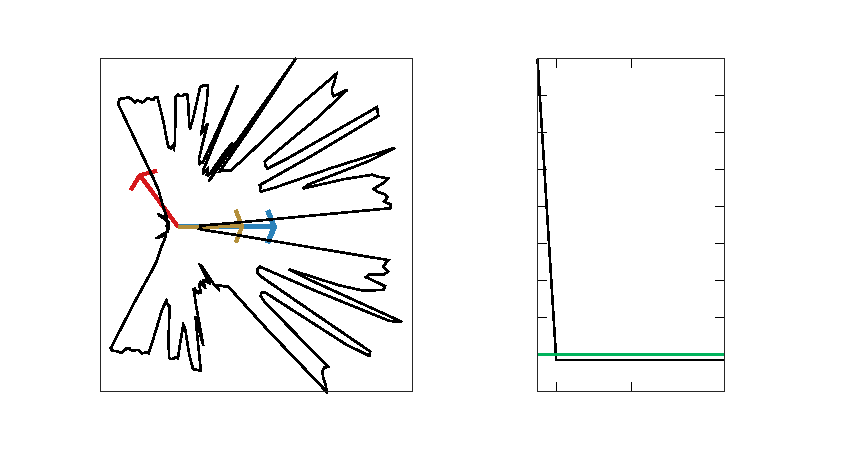
\includegraphics{./figures/parts/02/chapters/04/sections/02/rc_uf}}%
    \gplfronttext
  \end{picture}%
\endgroup

  \vspace{0.5cm}
  \caption{\small Αριστερά: η αρχική
           $\hat{\bm{p}}[0] \equiv (\bm{l},\hat{\theta}[0])$ και τελική
           $\hat{\bm{p}}[1] \equiv (\bm{l},\hat{\theta}[1])$ εκτίμηση στάσης του
           αισθητήρα σε ένα περιβάλλον με χάρτη $\bm{M}$, για πραγματική στάση
           $\bm{p}(\bm{l},\theta)$, ως συνέπεια της εφαρμογής της μεθόδου
           γωνιακής ευθυγράμμισης Προκρούστη. Δεξιά: το σφάλμα εκτίμησης
           προσανατολισμού ως συνάρτηση της διακριτικής γωνίας $\gamma$ του
           αισθητήρα}
  \label{fig:02_04_02:rc_uf}
\end{figure}


\begin{algorithm}[h]
  \caption{\texttt{rc\_uf}}
  \begin{spacing}{1.3}
  \begin{algorithmic}[1]
    \REQUIRE $\mathcal{S}_R$, $\mathcal{S}_V$, $\hat{\bm{p}}(x, y, \hat{\theta})$, $\gamma$
    \ENSURE $\hat{\theta}^\prime$, $T$
    %\STATE $\mathcal{S}_V \leftarrow \texttt{scan\_map}(\bm{M}, \hat{\bm{p}}, N_s)$
    \STATE $\bm{P}_R \leftarrow \texttt{project}(\mathcal{S}_R, (0,0,0))$
    \STATE $\bm{P}_V \leftarrow \texttt{project}(\mathcal{S}_V, (0,0,0))$
    \STATE $(J,T) \leftarrow \texttt{rc\_uf\_core}(\bm{P}_R, \bm{P}_V)$ (Αλγόριθμος \ref{alg:algorithm_core_ufrc})
    \STATE $N_s = 2 \pi / \gamma$
    \STATE $\psi = N_s - 1 - J$
    \STATE $\hat{\theta}^\prime \leftarrow \hat{\theta} + \psi \gamma$
    \RETURN $(\hat{\theta}^\prime, T)$
  \end{algorithmic}
  \end{spacing}
  \label{alg:algorithm_ufrc}
\end{algorithm}


\begin{algorithm}[h]
  \caption{\texttt{rc\_uf\_core}}
  \begin{spacing}{1.3}
  \begin{algorithmic}[1]
    \REQUIRE $\bm{P}_R$, $\bm{P}_V$
    \ENSURE $J$, $T(\bm{P}_R, \bm{P}_V)$
    \STATE \texttt{reverse}$(\bm{P}_V)$
    \STATE $\bm{p}_R^x \leftarrow \text{first row of } \bm{P}_R$
    \STATE $\bm{p}_R^y \leftarrow \text{second row of } \bm{P}_R$
    \STATE $\bm{p}_V^x \leftarrow \text{first row of } \bm{P}_V$
    \STATE $\bm{p}_V^y \leftarrow \text{second row of } \bm{P}_V$
    \STATE $\bm{m}_{11} \leftarrow \mathcal{F}^{-1}\{\mathcal{F}\{\bm{p}_R^x\} \odot \mathcal{F}\{\bm{p}_V^x\}\}$
    \STATE $\bm{m}_{12} \leftarrow \mathcal{F}^{-1}\{\mathcal{F}\{\bm{p}_R^y\} \odot \mathcal{F}\{\bm{p}_V^x\}\}$
    \STATE $\bm{m}_{21} \leftarrow \mathcal{F}^{-1}\{\mathcal{F}\{\bm{p}_R^x\} \odot \mathcal{F}\{\bm{p}_V^y\}\}$
    \STATE $\bm{m}_{22} \leftarrow \mathcal{F}^{-1}\{\mathcal{F}\{\bm{p}_R^y\} \odot \mathcal{F}\{\bm{p}_V^y\}\}$
    \STATE $\bm{T} \leftarrow \{\varnothing\}$
    \FOR{\texttt{$j = 0:N_s-1$}}
      \vspace{0.1cm}
      \STATE $\bm{M}_j \leftarrow
        \begin{bmatrix}
          \bm{m}_{11}(j) & \bm{m}_{12}(j) \\
          \bm{m}_{21}(j) & \bm{m}_{22}(j)
        \end{bmatrix}$
        \vspace{0.1cm}
        \STATE $(\bm{U}, \bm{D}, \bm{V}) \leftarrow \texttt{SVD}(\bm{M}_j)$
        \STATE \texttt{append} $\texttt{trace}(\bm{D} \cdot \texttt{diag}(1,\det(\bm{U}\bm{V})))$ to $\bm{T}$
    \ENDFOR
    \STATE \texttt{reverse}$(\bm{T})$
    \STATE $J \leftarrow \arg\max\bm{T}$
    \STATE $T_{\max} \leftarrow \max \{\bm{T}\} = \bm{T}[J]$
    \RETURN $(J,T_{\max})$
  \end{algorithmic}
  \end{spacing}
  \label{alg:algorithm_core_ufrc}
\end{algorithm}




%%%%%%%%%%%%%%%%%%%%%%%%%%%%%%%%%%%%%%%%%%%%%%%%%%%%%%%%%%%%%%%%%%%%%%%%%%%%%%%%
\subsection{Η κλίνη της διακριτικής γωνίας του αισθητήρα}
\label{subsection:02_04_02:04}

Η μέθοδος Fourier-Mellin σε μία διάσταση (ενότητα \ref{subsection:02_04_02:01})
και η μέθοδος του Προκρούστη (ενότητα \ref{subsection:02_04_02:03}), σε
αντίθεση με την μέθοδο Πρώτων Αρχών (ενότητα \ref{subsection:02_04_02:02}),
είναι διακριτές μέθοδοι εκτίμησης υπό την έννοια ότι λειτουργούν
\textit{μειώνοντας την αρχική εκτίμηση προσανατολισμού κατά ακέραια πολλαπλάσια
της σταθεράς διακριτικής γωνίας $\gamma$}, με αποτέλεσμα αυθαίρετα επίλοιπα
σφάλματα προσανατολισμού $\phi$ όπως ορίζονται από τα Λήμματα
\ref{lemma:02_04_02:01} και \ref{lemma:02_04_02:03}. Αυτός ο περιορισμός
μπορεί να ιδωθεί ως μία έτερη Προκρούστεια ιδιότητα,\footnote{Στη μυθολογία ο
Πολυπήμων, γνωστότερος ως Προκρούστης, ήταν ένας απαγωγέας ξένων, και μάστιγα
της Ιεράς Οδού της Αττικής. Αφού φιλοξενούσε τα θύματά του προσφέροντάς τούς
ένα πλουσιοπάροχο δείπνο, τα προσκαλούσε να ξαπλώσουν σε ένα κρεβάτι διαστάσεων
τέτοιων που το ύψος του θύματος καλείτο να προσαρμοστεί στο μήκος του
κρεβατιού, είτε μέσω τεμαχισμού του σώματός του, είτε μέσω τάνυσής του. Ο
Πολυπήμων είχε την ατυχία να απαγάγει τον Θησέα, ο οποίος, άρτι αφιχθείς από τη
δολοφονία του Μινώταυρου, τον τιμώρησε χρησιμοποιώντας την τεχνική του εναντίον
τού.} που αφορά σε δύο μεθόδους αυτή τη φορά, υπό την έννοια ότι το αρχικό
σφάλμα προσανατολισμού $|\theta - \hat{\theta}| \in \mathbb{R}_{\geq 0}$
τεμαχίζεται στην κλίνη $K\gamma, K \in \mathbb{Z}_{\geq 0}$, στη βάση διακριτής
και εξωτερικής λογικής:---το αρχικό σφάλμα προσαρμόζεται στη μέθοδο, αντί η
μέθοδος να είναι προσαρμόσιμη στο αρχικό σφάλμα.

Επιπρόσθετα, σύμφωνα με τα Λήμματα \ref{lemma:02_04_02:01},
\ref{lemma:02_04_02:02}, και \ref{lemma:02_04_02:03} τα τελικά σφάλματα
προσανατολισμού των τριών ως άνω μεθόδων εξαρτώνται από τον \textit{αμετάβλητο}
αριθμό των εκπεμπόμενων από τον φυσικό αισθητήρα απόστασης ακτίνων, ή,
ισοδύναμα, από την αμετάβλητη διακριτική του γωνία $\gamma$. Το πεπερασμένο και
αμετάβλητο των εκπεμπόμενων ακτίνων του φυσικού αισθητήρα, σε συνδυασμό με το
αυθαίρετο του ρυθμού των αλλαγών του περιβάλλοντος (σχήμα
\ref{fig:02_02:the_problem}), μπορούν να οδηγήσουν σε υποδειγματοληψία τμημάτων
του περιβάλλοντος ή/και του χάρτη του, με συνέπεια τη μη βέλτιστη σύγκλιση της
εκτίμησης προσανατολισμού.

Οι δύο παραπάνω παρατηρήσεις αφορούν στα σφάλματα στάσης της συνολικής μεθόδου
ευθυγράμμισης, όχι μόνο λόγω των μη επιλύσιμων σφαλμάτων προσανατολισμού αυτών
καθεαυτά, αλλά και λόγω της διάδοσής τους στην διαδεχόμενη της μεθόδου
ευθυγράμμισης προσανατολισμού μέθοδο ευθυγράμμισης της θέσης (Παρατήρηση
\ref{rem:iterative}): λόγω σύζευξης των δύο ειδών ευθυγράμμισης, η μέθοδος
εκτίμησης θέσης απαιτεί επί της αρχής μηδενικά σφάλματα προσανατολισμού. Κατ'
ελάχιστον, όμως, στην περίπτωση των δύο ως άνω Προκρούστειων μεθόδων, το τελικό
σφάλμα προσανατολισμού τους μπορεί να έχει τιμή έως και $\gamma/2$. Για την
επίλυση αυτού του προβλήματος εξετάζουμε δύο υποψήφιες μεθόδους, οι οποίες
παρουσιάζονται στις επόμενες δύο ενότητες.


%%%%%%%%%%%%%%%%%%%%%%%%%%%%%%%%%%%%%%%%%%%%%%%%%%%%%%%%%%%%%%%%%%%%%%%%%%%%%%%%
\subsection{Η μέθοδος του Πιτυοκάμπτη Σίνι}
\label{subsection:02_04_02:05}

Προτού εισάγουμε τη μέθοδο που ελαττώνει τα σφάλματα εκτίμησης προσανατολισμού
που προτείνουμε, πρέπει να εξετάσουμε το λόγο για την πολυπλοκότητά και την
επιτυχία της σε σχέση με την αφελή μέθοδο επιχείρησης ελάττωσης του σφάλματος
εκτίμησης του προσανατολισμού, η οποία παρουσιάζεται στην παρούσα ενότητα.

Δεδομένων ότι

\begin{itemize}
  \item το τελικό σφάλμα εκτίμησης προσανατολισμού των τριών ως άνω
        μεθόδων είναι αντιστρόφως ανάλογο του αριθμού εκπεμπομένων ακτίνων $N_s$
  \item ο τελευταίος είναι \textit{αμετάβλητος} όσο αφορά στον φυσικό αισθητήρα
        αποστάσεων (με την έννοια ότι δεν μπορεί να προσδώσει περισσότερες
        μετρήσεις από $N_s = 2\pi/\gamma$)
  \item o τελευταίος είναι \textit{μεταβλητός} όσο αφορά στον εικονικό αισθητήρα
        αποστάσεων (με την έννοια ότι, εφόσον οι εικονικές σαρώσεις είναι
        υπολογιστέες μέσω του χάρτη, μπορεί να υπολογιστεί ένας αυθαίρετος
        αριθμός εικονικών ακτίνων εντός του)
\end{itemize}
ένας αφελής τρόπος επίλυσης του προβλήματος ελάττωσης του σφάλματος
προσανατολισμού συνίσταται στην αύξηση των εκπεμπόμενων ακτίνων
\begin{itemize}
  \item του φυσικού αισθητήρα με την παρεμβολή των τιμών των ακτίνων της
        πραγματικής σάρωσης
  \item του εικονικού αισθητήρα με την δεσμοβολή ισάριθμων ακτίνων της
        πραγματικής σάρωσης εντός του χάρτη $\bm{M}$
\end{itemize}

Σε αυτή την περίπτωση η αύξηση του αριθμού των ακτίνων της πραγματικής σάρωσης
μέσω παρεμβολής γίνεται με διχοτόμηση όλων των $N_s$ γωνιών μεταξύ γειτονικών
ακτίνων, και εισαγωγή ακτίνων σε γωνίες
$n\gamma + \gamma/2$, $n = 0,1,\dots,N_s-1$, των οποίων η αναφερόμενη απόσταση
τίθεται σε
$\mathcal{S}_R^{\prime\text{\ interp}}[n] = \dfrac{1}{2}(\mathcal{S}_R[n] + \mathcal{S}_R[n+1])$,
όπου $\mathcal{S}_R[N_s] = \mathcal{S}_R[0]$. Με αυτόν τον τρόπο
η προκύπτουσα διακριτική γωνία είναι $\gamma^\prime = \gamma / 2$. Αυτή
διαδικασία θα μπορούσε να επαναληφθεί περαιτέρω, έως ότου η τελική
διακριτική γωνία φτάσει σε ένα αποδεκτά χαμηλό επίπεδο
$\gamma^{(\nu)} = \gamma / 2^\nu$, $\nu \in \mathbb{Z}_{> 0}$. Όσο αφορά στην
εικονική σάρωση, δεδομένου ότι παράγεται από το χάρτη, δεν απαιτεί τη χρήση
παρεμβολής---ο αριθμός των απαιτούμενων εικονικών ακτίνων $N_s^\prime$
καθορίζεται από το μέγεθος της πραγματικής σάρωσης: $N_s^\prime = 2^\nu N_s$.
Λόγω της χρήσης της τεχνικής διχοτόμησης ακτίνων ονομάζουμε αυτή τη μέθοδο ως
μέθοδο του Πιτυοκάμπτη Σίνι.\footnote{Ο Σίνις, επονομαζόμενος Πιτυοκάμπτης, ήταν
γιος του Προκρούστη Πολυπήμωνος. Σε συνέχεια της γενεαλογίας του ο Σίνις απήγαγε
ξένους, των οποίων τα άκρα έδενε σε δύο λυγισμένα πεύκα (κεκαμμένες πιτύες)
προτού αφήσει τα τελευταία να πάρουν τη φυσική τους κλίση, διχοτομώντας έτσι τα
σώματά των θυμάτων του. Για κακή του τύχη εξοντώθηκε επίσης από τον Θησέα.}

\begin{remark}
  \label{rem:sizes_incorrect}
  Κατά τη διάρκεια αυτής της μεθόδου ελάττωσης του σφάλματος προσανατολισμού η
  πραγματική σάρωση και ο χάρτης δειγματοληπτούνται με ρυθμό δειγματοληψίας
  $2^\nu$, με αποτέλεσμα \textit{μία} πραγματική σάρωση και \textit{μία}
  εικονική σάρωση, αποτελούμενες από $2^\nu N_s$ ακτίνες. Η διόρθωση
  προσανατολισμού εκτελείται \textit{μία} φορά, και έχει ως αποτέλεσμα
  \textit{μία} εκτίμηση προσανατολισμού.
\end{remark}

Στο σχήμα \ref{fig:oversampling_goes_wrong} απεικονίζεται μία μεγέθυνση των δύο
περιοχών του σχήματος \ref{fig:02_02:the_problem} που περικλείονται σε κόκκινα
και πράσινα πλαίσια. Η παραπάνω μεθοδολογία υπερδειγματοληψίας προσομοιώνει
τέλεια τις επιπρόσθετες αποστάσεις που θα λάμβανε ένας αισθητήρας με $2^2 N_s$
ακτίνες σε σχέση με έναν αισθητήρα $N_s$ ακτίνων σε γραμμικά τμήματα του
περιβάλλοντος (επάνω σειρά). Όμως, σε μη γραμμικά ή απότομα μεταβαλλόμενα
τμήματα του περιβάλλοντος (κάτω σειρά), η μέθοδος παρεμβολής αστοχεί στην
προσομοίωση των επιπρόσθετων αποστάσεων λόγω εισαγωγής σφαλμάτων απόστασης που
οφείλονται στην επινόηση τεχνητών μετρήσεων. Το μέγεθος αυτών των σφαλμάτων
εξαρτάται από το μέγεθος της διακριτικής γωνίας του αισθητήρα, τον ρυθμό
υπερδειγματοληψίας, και τον χάρτη ως ανεξάρτητη μεταβλητή.

\begin{figure}[h]\centering
  \vspace{0.5cm}
  \definecolor{sr}{RGB}{255,0,0}
\definecolor{sv}{RGB}{0,115,189}
\definecolor{sri}{RGB}{255,0,255}
\definecolor{svi}{RGB}{0,115,189}

% GNUPLOT: LaTeX picture with Postscript
\begingroup
  \makeatletter
  \providecommand\color[2][]{%
    \GenericError{(gnuplot) \space\space\space\@spaces}{%
      Package color not loaded in conjunction with
      terminal option `colourtext'%
    }{See the gnuplot documentation for explanation.%
    }{Either use 'blacktext' in gnuplot or load the package
      color.sty in LaTeX.}%
    \renewcommand\color[2][]{}%
  }%
  \providecommand\includegraphics[2][]{%
    \GenericError{(gnuplot) \space\space\space\@spaces}{%
      Package graphicx or graphics not loaded%
    }{See the gnuplot documentation for explanation.%
    }{The gnuplot epslatex terminal needs graphicx.sty or graphics.sty.}%
    \renewcommand\includegraphics[2][]{}%
  }%
  \providecommand\rotatebox[2]{#2}%
  \@ifundefined{ifGPcolor}{%
    \newif\ifGPcolor
    \GPcolorfalse
  }{}%
  \@ifundefined{ifGPblacktext}{%
    \newif\ifGPblacktext
    \GPblacktexttrue
  }{}%
  % define a \g@addto@macro without @ in the name:
  \let\gplgaddtomacro\g@addto@macro
  % define empty templates for all commands taking text:
  \gdef\gplfronttext{}%
  \gdef\gplfronttext{}%
  \makeatother
  \ifGPblacktext
    % no textcolor at all
    \def\colorrgb#1{}%
    \def\colorgray#1{}%
  \else
    % gray or color?
    \ifGPcolor
      \def\colorrgb#1{\color[rgb]{#1}}%
      \def\colorgray#1{\color[gray]{#1}}%
      \expandafter\def\csname LTw\endcsname{\color{white}}%
      \expandafter\def\csname LTb\endcsname{\color{black}}%
      \expandafter\def\csname LTa\endcsname{\color{black}}%
      \expandafter\def\csname LT0\endcsname{\color[rgb]{1,0,0}}%
      \expandafter\def\csname LT1\endcsname{\color[rgb]{0,1,0}}%
      \expandafter\def\csname LT2\endcsname{\color[rgb]{0,0,1}}%
      \expandafter\def\csname LT3\endcsname{\color[rgb]{1,0,1}}%
      \expandafter\def\csname LT4\endcsname{\color[rgb]{0,1,1}}%
      \expandafter\def\csname LT5\endcsname{\color[rgb]{1,1,0}}%
      \expandafter\def\csname LT6\endcsname{\color[rgb]{0,0,0}}%
      \expandafter\def\csname LT7\endcsname{\color[rgb]{1,0.3,0}}%
      \expandafter\def\csname LT8\endcsname{\color[rgb]{0.5,0.5,0.5}}%
    \else
      % gray
      \def\colorrgb#1{\color{black}}%
      \def\colorgray#1{\color[gray]{#1}}%
      \expandafter\def\csname LTw\endcsname{\color{white}}%
      \expandafter\def\csname LTb\endcsname{\color{black}}%
      \expandafter\def\csname LTa\endcsname{\color{black}}%
      \expandafter\def\csname LT0\endcsname{\color{black}}%
      \expandafter\def\csname LT1\endcsname{\color{black}}%
      \expandafter\def\csname LT2\endcsname{\color{black}}%
      \expandafter\def\csname LT3\endcsname{\color{black}}%
      \expandafter\def\csname LT4\endcsname{\color{black}}%
      \expandafter\def\csname LT5\endcsname{\color{black}}%
      \expandafter\def\csname LT6\endcsname{\color{black}}%
      \expandafter\def\csname LT7\endcsname{\color{black}}%
      \expandafter\def\csname LT8\endcsname{\color{black}}%
    \fi
  \fi
    \setlength{\unitlength}{0.0500bp}%
    \ifx\gptboxheight\undefined%
      \newlength{\gptboxheight}%
      \newlength{\gptboxwidth}%
      \newsavebox{\gptboxtext}%
    \fi%
    \setlength{\fboxrule}{0.5pt}%
    \setlength{\fboxsep}{1pt}%
\begin{picture}(5000.00,5000.00)%
    \gplgaddtomacro\gplfronttext{%
      \put(800,5000){\makebox(0,0){\strut{}{\color{sr}{\rule[0.6mm]{0.5cm}{0.5mm}}}               \small  $\mathcal{S}_R$}}
      \put(1800,5000){\makebox(0,0){\strut{}{\color{sv}{\rule[0.6mm]{0.5cm}{0.5mm}}}              \small  $\mathcal{S}_V$}}
      \put(3300,5000){\makebox(0,0){\strut{}{\color{sri}{\hdashrule[0.6mm]{0.65cm}{0.5mm}{0.5mm}}}\small  $\mathcal{S}_R^{\prime\text{\ interp}}$}}
      \put(4000,5000){\makebox(0,0){\strut{}{\color{svi}{\rule[0.6mm]{0.30cm}{0.5mm}}}}}
      \put(4350,5000){\makebox(0,0){\strut{}{\color{svi}{\hdashrule[0.6mm]{0.35cm}{0.5mm}{0.5mm}}}\small  $\mathcal{S}_V^\prime$}}

      \put(1400,-200){\makebox(0,0){\strut{}\small $|\mathcal{S}_R| = |\mathcal{S}_V| = N_s$}}
      \put(3700,-200){\makebox(0,0){\strut{}\small $|\mathcal{S}_R^\prime| = |\mathcal{S}_R| + |\mathcal{S}_R^{\prime\text{\ interp}}|$}}
      \put(3780,-500){\makebox(0,0){\strut{}\small $= |\mathcal{S}_V^\prime| = 2^2 N_s$}}
    }%
    \gplgaddtomacro\gplfronttext{%
    }%
    \gplgaddtomacro\gplfronttext{%
    }%
    \gplgaddtomacro\gplfronttext{%
    }%
    \gplgaddtomacro\gplfronttext{%
    }%
    \gplgaddtomacro\gplfronttext{%
    }%
    \gplgaddtomacro\gplfronttext{%
    }%
    \gplgaddtomacro\gplfronttext{%
    }%
    \put(0,0){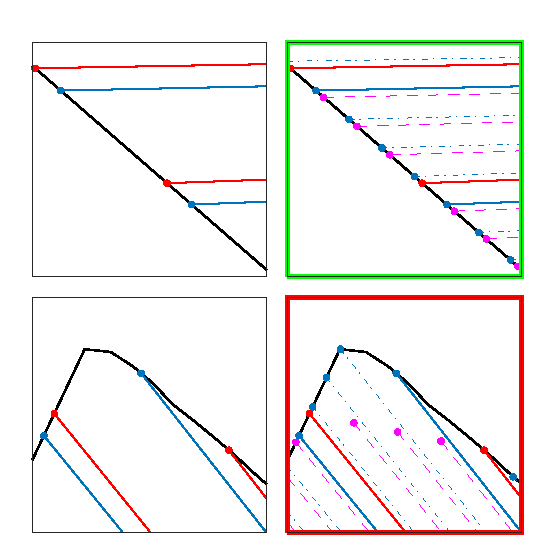
\includegraphics{./figures/parts/02/chapters/04/sections/02/false_oversampling}}%
    \gplfronttext
  \end{picture}%
\endgroup

  \vspace{1.0cm}
  \caption{\small Μεγέθυνση των δύο περιοχών που περικλείονται με κόκκινο
           και πράσινο χρώμα στο σχήμα \ref{fig:02_02:the_problem}. Οι κόκκινες
           γραμμές υποδηλώνουν ακτίνες της πραγματικής μέτρησης $\mathcal{S}_R$.
           Oι μπλε γραμμές υποδηλώνουν ακτίνες της εικονικής μέτρησης $\mathcal{S}_V$.
           Οι διακεκομμένες φούξια γραμμές απεικονίζουν τις παρεμβαλλόμενες
           ακτίνες του πραγματικού αισθητήρα. Οι διακεκομμένες μπλε γραμμές
           απεικονίζουν τις πρόσθετες ακτίνες του εικονικού αισθητήρα.
           Εδώ ο ρυθμός υπερδειγματοληψίας είναι $\mu = 2^\nu$, $\nu = 2$.
           Τα σχήματα στην αριστερή πλευρά δείχνουν τις αρχικές σαρώσεις
           μεγέθους $N_s$. Τα δεξιά σχήματα δείχνουν την παρεμβαλλόμενη
           πραγματική σάρωση και την εικονική σάρωση ίσου μεγέθους $N_s^\prime
           = 2^\nu N_s$. Η παρεμβολή των ακτίνων της πραγματικής σάρωσης είναι
           ακριβής σε γραμμικά τμήματα. Σε μη γραμμικά τµήµατα, όμως, οι
           αποστάσεις των παρεµβαλλόµενων ακτίνων είναι αυθαίρετα λανθασμένες,
           και δεν μπορεί να διασφαλιστεί ότι το σφάλμα προσανατολισμού
           φράσσεται άνωθεν από την τιμή $\gamma/2^{\nu+1}$. }
  \label{fig:oversampling_goes_wrong}
\end{figure}

Αυτό σημαίνει ότι η εισαγωγή παρεμβαλλόμενων ακτίνων έχει το αμετάβλητο και
ακούσιο αποτέλεσμα η λύση να εισάγει τα δικά της σφάλματα στην επιζητούμενη
εκτίμηση. Επιπλέον, αυτό το σφάλμα δεν μπορεί να ελεγχθεί, και, κατά συνέπεια,
είναι αναγκαία εναλλακτική προσέγγιση λύσης του προβλήματος. Για του λόγου το
αληθές, στο σχήμα \ref{fig:02_04_02:sinis} εκτίθεται το μέγεθος, η τυχαιότητα,
και η αστάθεια αυτών των σφαλμάτων. Όπως και πριν απεικονίζονται οι αρχικές και
τελικές συνθήκες ευθυγράμμισης προσανατολισμού για έναν αισθητήρα δισδιάστατων
πανοραμικών σαρώσεων με $\gamma = 2\pi/360$, σε ένα μη δομημένο περιβάλλον, του
οποίου ο χάρτης το αναπαριστά τέλεια, ενώ οι μετρήσεις του αισθητήρα δεν
διαταράσσονται από θόρυβο. H μέθοδος του Πιτυοκάμπτη Σίνι εφαρμόζεται επί των
μεθόδων Fourier-Mellin μίας διάστασης (άνω) και Προκρούστη (κάτω). Εδώ ο βαθμός
υπερδειγματοληψίας $\nu$ έχει αρχική τιμή $\nu = \nu_{\min} = 0$ και αυξάνει
διαδοχικά κάθε φορά που η εκτίμηση προσανατολισμού δεν εμφανίζει μεταβολή ως
προς την προηγούμενη τιμή της πάνω από $\gamma/2$ rad, έως ότου $\nu =
\nu_{\max} = 3$.

\begin{figure}[h]\centering
  \definecolor{sr}{RGB}{43,131,186}
\definecolor{svi}{RGB}{215,25, 28}
\definecolor{svf}{RGB}{179,143,59}
\definecolor{g}{RGB}{0,178,93}
\definecolor{k}{RGB}{0,0,0}
\definecolor{m}{RGB}{255,0,255}

% GNUPLOT: LaTeX picture with Postscript
\begingroup
  \makeatletter
  \providecommand\color[2][]{%
    \GenericError{(gnuplot) \space\space\space\@spaces}{%
      Package color not loaded in conjunction with
      terminal option `colourtext'%
    }{See the gnuplot documentation for explanation.%
    }{Either use 'blacktext' in gnuplot or load the package
      color.sty in LaTeX.}%
    \renewcommand\color[2][]{}%
  }%
  \providecommand\includegraphics[2][]{%
    \GenericError{(gnuplot) \space\space\space\@spaces}{%
      Package graphicx or graphics not loaded%
    }{See the gnuplot documentation for explanation.%
    }{The gnuplot epslatex terminal needs graphicx.sty or graphics.sty.}%
    \renewcommand\includegraphics[2][]{}%
  }%
  \providecommand\rotatebox[2]{#2}%
  \@ifundefined{ifGPcolor}{%
    \newif\ifGPcolor
    \GPcolorfalse
  }{}%
  \@ifundefined{ifGPblacktext}{%
    \newif\ifGPblacktext
    \GPblacktexttrue
  }{}%
  % define a \g@addto@macro without @ in the name:
  \let\gplgaddtomacro\g@addto@macro
  % define empty templates for all commands taking text:
  \gdef\gplfronttext{}%
  \gdef\gplfronttext{}%
  \makeatother
  \ifGPblacktext
    % no textcolor at all
    \def\colorrgb#1{}%
    \def\colorgray#1{}%
  \else
    % gray or color?
    \ifGPcolor
      \def\colorrgb#1{\color[rgb]{#1}}%
      \def\colorgray#1{\color[gray]{#1}}%
      \expandafter\def\csname LTw\endcsname{\color{white}}%
      \expandafter\def\csname LTb\endcsname{\color{black}}%
      \expandafter\def\csname LTa\endcsname{\color{black}}%
      \expandafter\def\csname LT0\endcsname{\color[rgb]{1,0,0}}%
      \expandafter\def\csname LT1\endcsname{\color[rgb]{0,1,0}}%
      \expandafter\def\csname LT2\endcsname{\color[rgb]{0,0,1}}%
      \expandafter\def\csname LT3\endcsname{\color[rgb]{1,0,1}}%
      \expandafter\def\csname LT4\endcsname{\color[rgb]{0,1,1}}%
      \expandafter\def\csname LT5\endcsname{\color[rgb]{1,1,0}}%
      \expandafter\def\csname LT6\endcsname{\color[rgb]{0,0,0}}%
      \expandafter\def\csname LT7\endcsname{\color[rgb]{1,0.3,0}}%
      \expandafter\def\csname LT8\endcsname{\color[rgb]{0.5,0.5,0.5}}%
    \else
      % gray
      \def\colorrgb#1{\color{black}}%
      \def\colorgray#1{\color[gray]{#1}}%
      \expandafter\def\csname LTw\endcsname{\color{white}}%
      \expandafter\def\csname LTb\endcsname{\color{black}}%
      \expandafter\def\csname LTa\endcsname{\color{black}}%
      \expandafter\def\csname LT0\endcsname{\color{black}}%
      \expandafter\def\csname LT1\endcsname{\color{black}}%
      \expandafter\def\csname LT2\endcsname{\color{black}}%
      \expandafter\def\csname LT3\endcsname{\color{black}}%
      \expandafter\def\csname LT4\endcsname{\color{black}}%
      \expandafter\def\csname LT5\endcsname{\color{black}}%
      \expandafter\def\csname LT6\endcsname{\color{black}}%
      \expandafter\def\csname LT7\endcsname{\color{black}}%
      \expandafter\def\csname LT8\endcsname{\color{black}}%
    \fi
  \fi
    \setlength{\unitlength}{0.0500bp}%
    \ifx\gptboxheight\undefined%
      \newlength{\gptboxheight}%
      \newlength{\gptboxwidth}%
      \newsavebox{\gptboxtext}%
    \fi%
    \setlength{\fboxrule}{0.5pt}%
    \setlength{\fboxsep}{1pt}%
\begin{picture}(8000.00,8000.00)%
    \gplgaddtomacro\gplfronttext{%
    }%
    \gplgaddtomacro\gplfronttext{%
    }%
    \gplgaddtomacro\gplfronttext{%
      \colorrgb{0.15,0.15,0.15}%
      \put(4868,4400){\makebox(0,0)[r]{\strut{}$2^{-2}$}}%
      \colorrgb{0.15,0.15,0.15}%
      \put(4868,4680){\makebox(0,0)[r]{\strut{}$2^{-1}$}}%
      \colorrgb{0.15,0.15,0.15}%
      \put(4868,4960){\makebox(0,0)[r]{\strut{}$2^{0}$}}%
      \colorrgb{0.15,0.15,0.15}%
      \put(4868,5240){\makebox(0,0)[r]{\strut{}$2^{1}$}}%
      \colorrgb{0.15,0.15,0.15}%
      \put(4868,5520){\makebox(0,0)[r]{\strut{}$2^{2}$}}%
      \colorrgb{0.15,0.15,0.15}%
      \put(4868,5800){\makebox(0,0)[r]{\strut{}$2^{3}$}}%
      \colorrgb{0.15,0.15,0.15}%
      \put(4868,6080){\makebox(0,0)[r]{\strut{}$2^{4}$}}%
      \colorrgb{0.15,0.15,0.15}%
      \put(4868,6360){\makebox(0,0)[r]{\strut{}$2^{5}$}}%
      \colorrgb{0.15,0.15,0.15}%
      \put(4868,6640){\makebox(0,0)[r]{\strut{}$2^{6}$}}%
      \colorrgb{0.15,0.15,0.15}%
      \put(4868,6921){\makebox(0,0)[r]{\strut{}$2^{7}$}}%
      \colorrgb{0.15,0.15,0.15}%
      \put(4868,7201){\makebox(0,0)[r]{\strut{}$2^{8}$}}%
      \colorrgb{0.15,0.15,0.15}%
      \put(5095,4180){\makebox(0,0){\strut{}$1$}}%
      \colorrgb{0.15,0.15,0.15}%
      \put(6231,4180){\makebox(0,0){\strut{}$13$}}%
      \colorrgb{0.15,0.15,0.15}%
      \put(6515,4180){\makebox(0,0){\strut{}$16$}}%
      \colorrgb{0.15,0.15,0.15}%
      \put(6799,4180){\makebox(0,0){\strut{}$19$}}%
    }%
    \gplgaddtomacro\gplfronttext{%
    }%
    \gplgaddtomacro\gplfronttext{%
    }%
    \gplgaddtomacro\gplfronttext{%
    }%
    \gplgaddtomacro\gplfronttext{%
      \colorrgb{0.15,0.15,0.15}%
      \put(4868,800){\makebox(0,0)[r]{\strut{}$2^{-2}$}}%
      \colorrgb{0.15,0.15,0.15}%
      \put(4868,1080){\makebox(0,0)[r]{\strut{}$2^{-1}$}}%
      \colorrgb{0.15,0.15,0.15}%
      \put(4868,1360){\makebox(0,0)[r]{\strut{}$2^{0}$}}%
      \colorrgb{0.15,0.15,0.15}%
      \put(4868,1640){\makebox(0,0)[r]{\strut{}$2^{1}$}}%
      \colorrgb{0.15,0.15,0.15}%
      \put(4868,1920){\makebox(0,0)[r]{\strut{}$2^{2}$}}%
      \colorrgb{0.15,0.15,0.15}%
      \put(4868,2200){\makebox(0,0)[r]{\strut{}$2^{3}$}}%
      \colorrgb{0.15,0.15,0.15}%
      \put(4868,2480){\makebox(0,0)[r]{\strut{}$2^{4}$}}%
      \colorrgb{0.15,0.15,0.15}%
      \put(4868,2760){\makebox(0,0)[r]{\strut{}$2^{5}$}}%
      \colorrgb{0.15,0.15,0.15}%
      \put(4868,3040){\makebox(0,0)[r]{\strut{}$2^{6}$}}%
      \colorrgb{0.15,0.15,0.15}%
      \put(4868,3321){\makebox(0,0)[r]{\strut{}$2^{7}$}}%
      \colorrgb{0.15,0.15,0.15}%
      \put(4868,3601){\makebox(0,0)[r]{\strut{}$2^{8}$}}%
      \colorrgb{0.15,0.15,0.15}%
      \put(5078,580){\makebox(0,0){\strut{}$1$}}%
      \colorrgb{0.15,0.15,0.15}%
      \put(5548,580){\makebox(0,0){\strut{}$7$}}%
      \colorrgb{0.15,0.15,0.15}%
      \put(6173,580){\makebox(0,0){\strut{}$15$}}%
      \colorrgb{0.15,0.15,0.15}%
      \put(6799,580){\makebox(0,0){\strut{}$23$}}%
    }%
    \gplgaddtomacro\gplfronttext{%
      \colorrgb{0.15,0.15,0.15}%
      \put(5400,7519){\makebox(0,0){\strut{}{\color{k}{\rule[0.6mm]{0.5cm}{0.5mm}}} $\dfrac{|\theta-\hat{\theta}[k]|}{\gamma}$}}%
      \put(6700,7519){\makebox(0,0){\strut{}{\color{g}{\rule[0.6mm]{0.5cm}{0.5mm}}} $2^{-1}$}}%
      \put(1100,7519){\makebox(0,0){\strut{}{\color{k}{\rule[0.6mm]{0.5cm}{0.5mm}}} $\bm{M}$}}%
      \put(1850,7519){\makebox(0,0){\strut{}{\color{sr}{\rule[0.6mm]{0.5cm}{0.5mm}}} $\bm{p}$}}%
      \put(2600,7519){\makebox(0,0){\strut{}{\color{svi}{\rule[0.6mm]{0.5cm}{0.5mm}}} $\hat{\bm{p}}[0]$}}%
      \put(3600,7519){\makebox(0,0){\strut{}{\color{svf}{\rule[0.6mm]{0.5cm}{0.5mm}}} $\hat{\bm{p}}[k_{\max}]$}}%

      \put(5100,3869){\makebox(0,0){\strut{}$\nu$}}%
      \put(5400,3869){\makebox(0,0){\strut{}\fcolorbox{black}{sinisn0}{\rule{0pt}{6pt}\rule{6pt}{0pt} 0}}} %
      \put(5800,3869){\makebox(0,0){\strut{}\fcolorbox{black}{sinisn1}{\rule{0pt}{6pt}\rule{6pt}{0pt} 1}}} %
      \put(6200,3869){\makebox(0,0){\strut{}\fcolorbox{black}{sinisn2}{\rule{0pt}{6pt}\rule{6pt}{0pt} 2}}} %
      \put(6600,3869){\makebox(0,0){\strut{}\fcolorbox{black}{sinisn3}{\rule{0pt}{6pt}\rule{6pt}{0pt} 3}}} %

      \put(2300,4039){\makebox(0,0){\strut{} \texttt{rc\_fm}}}%
      \put(2300,250){\makebox(0,0){\strut{} \texttt{rc\_uf}}}%

      \put(5899,250){\makebox(0,0){\strut{}Αριθμός επαναλήψεων $k$}}%
    }
    \put(0,0){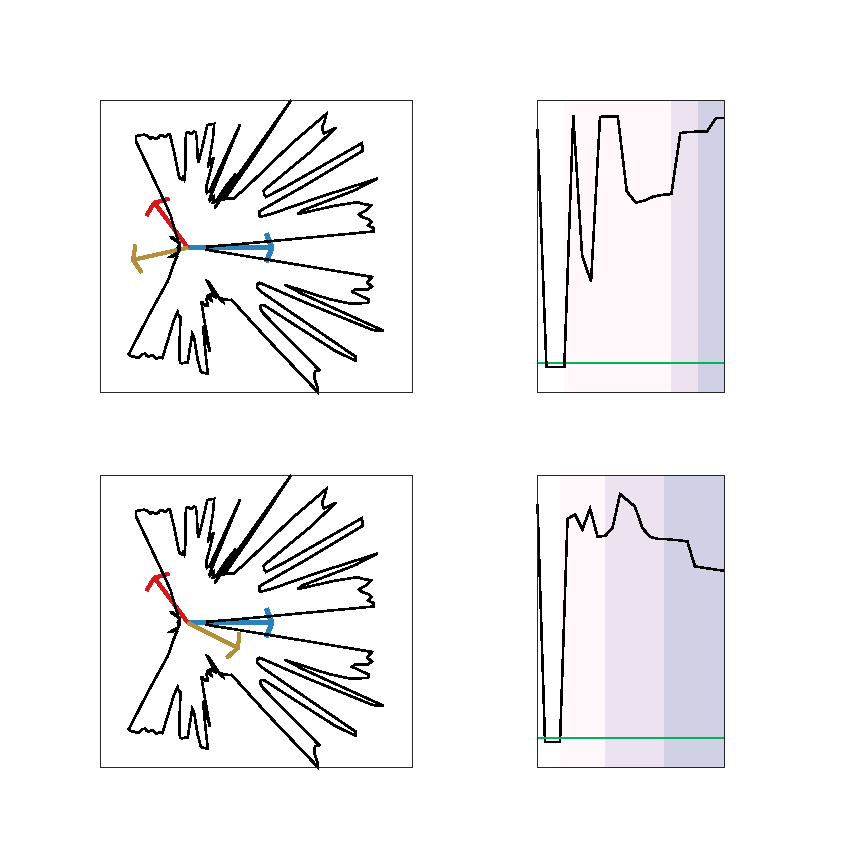
\includegraphics{./figures/parts/02/chapters/04/sections/02/sinis}}%
    \gplfronttext
  \end{picture}%
\endgroup

  \caption{\small Η λανθασμένη προσέγγιση ελάττωσης του γωνιακού σφάλματος
           εκτίμησης της μεθόδου Πιτυοκάμπτη Σίνι για διαδοχική
           υπερδειγματοληψία βαθμών $(\nu_{\min}, \nu_{\max}) = (0,3)$. Το
           σφάλμα εκτίμησης προσανατολισμού $\phi^{(\nu)}$ φράσσεται από την
           ποσότητα $\gamma/2^{1+\nu}$ μόνο στο τέλος του βήματος
           δειγματοληψίας $\nu=0$}
  \label{fig:02_04_02:sinis}
\end{figure}

Στην ενότητα \ref{subsection:02_04_02:06} παρουσιάζουμε τη μέθοδο που, σε
αντίθεση με τη μέθοδο του Πιτυοκάμπτη Σίνι, ελαττώνει το σφάλμα εκτίμησης
προσανατολισμού με τρόπο ευσταθή, προβλεπόμενο, και αναλογικό ως προς το ρυθμό
δειγματοληψίας $\mu = 2^{\nu}$ του χάρτη $\bm{M}$.

%%%%%%%%%%%%%%%%%%%%%%%%%%%%%%%%%%%%%%%%%%%%%%%%%%%%%%%%%%%%%%%%%%%%%%%%%%%%%%%%
\subsection{Η μέθοδος του Θησέα}
\label{subsection:02_04_02:06}

Από την παραπάνω ανάλυση γίνεται κατανοητό ότι οποιαδήποτε προσπάθεια
μείωσης του σφάλματος εκτίμησης προσανατολισμού θα πρέπει να περιοριστεί από
την απαγόρευση εφεύρεσης πραγματικών μετρήσεων. Στο σχήμα
\ref{fig:oversampling_correct} απεικονίζεται η μεθοδολογία που εισάγουμε, η
οποία εγγυάται ότι το τελικό σφάλμα προσανατολισμού $|\phi| \in [0,\gamma /
2^{1+\nu}]$ στην περίπτωση που οι μετρήσεις του φυσικού αισθητήρα δεν
διαταράσσονται από θόρυβο και ο χάρτης αναπαριστά το περιβάλλον τέλεια, για
$\nu = 2$ και $\gamma = 2\pi/360$.

\begin{figure}[h]\centering
  % GNUPLOT: LaTeX picture with Postscript

\definecolor{BL}{rgb}{0, 0.4470, 0.7410}
\definecolor{OR}{rgb}{0.6500, 0.3250, 0.1980}
\definecolor{GR}{rgb}{0.4660, 0.7740, 0.2880}
\definecolor{PU}{rgb}{0.4940, 0.1840, 0.5560}

\begingroup
  \makeatletter
  \providecommand\color[2][]{%
    \GenericError{(gnuplot) \space\space\space\@spaces}{%
      Package color not loaded in conjunction with
      terminal option `colourtext'%
    }{See the gnuplot documentation for explanation.%
    }{Either use 'blacktext' in gnuplot or load the package
      color.sty in LaTeX.}%
    \renewcommand\color[2][]{}%
  }%
  \providecommand\includegraphics[2][]{%
    \GenericError{(gnuplot) \space\space\space\@spaces}{%
      Package graphicx or graphics not loaded%
    }{See the gnuplot documentation for explanation.%
    }{The gnuplot epslatex terminal needs graphicx.sty or graphics.sty.}%
    \renewcommand\includegraphics[2][]{}%
  }%
  \providecommand\rotatebox[2]{#2}%
  \@ifundefined{ifGPcolor}{%
    \newif\ifGPcolor
    \GPcolorfalse
  }{}%
  \@ifundefined{ifGPblacktext}{%
    \newif\ifGPblacktext
    \GPblacktexttrue
  }{}%
  % define a \g@addto@macro without @ in the name:
  \let\gplgaddtomacro\g@addto@macro
  % define empty templates for all commands taking text:
  \gdef\gplfronttext{}%
  \gdef\gplfronttext{}%
  \makeatother
  \ifGPblacktext
    % no textcolor at all
    \def\colorrgb#1{}%
    \def\colorgray#1{}%
  \else
    % gray or color?
    \ifGPcolor
      \def\colorrgb#1{\color[rgb]{#1}}%
      \def\colorgray#1{\color[gray]{#1}}%
      \expandafter\def\csname LTw\endcsname{\color{white}}%
      \expandafter\def\csname LTb\endcsname{\color{black}}%
      \expandafter\def\csname LTa\endcsname{\color{black}}%
      \expandafter\def\csname LT0\endcsname{\color[rgb]{1,0,0}}%
      \expandafter\def\csname LT1\endcsname{\color[rgb]{0,1,0}}%
      \expandafter\def\csname LT2\endcsname{\color[rgb]{0,0,1}}%
      \expandafter\def\csname LT3\endcsname{\color[rgb]{1,0,1}}%
      \expandafter\def\csname LT4\endcsname{\color[rgb]{0,1,1}}%
      \expandafter\def\csname LT5\endcsname{\color[rgb]{1,1,0}}%
      \expandafter\def\csname LT6\endcsname{\color[rgb]{0,0,0}}%
      \expandafter\def\csname LT7\endcsname{\color[rgb]{1,0.3,0}}%
      \expandafter\def\csname LT8\endcsname{\color[rgb]{0.5,0.5,0.5}}%
    \else
      % gray
      \def\colorrgb#1{\color{black}}%
      \def\colorgray#1{\color[gray]{#1}}%
      \expandafter\def\csname LTw\endcsname{\color{white}}%
      \expandafter\def\csname LTb\endcsname{\color{black}}%
      \expandafter\def\csname LTa\endcsname{\color{black}}%
      \expandafter\def\csname LT0\endcsname{\color{black}}%
      \expandafter\def\csname LT1\endcsname{\color{black}}%
      \expandafter\def\csname LT2\endcsname{\color{black}}%
      \expandafter\def\csname LT3\endcsname{\color{black}}%
      \expandafter\def\csname LT4\endcsname{\color{black}}%
      \expandafter\def\csname LT5\endcsname{\color{black}}%
      \expandafter\def\csname LT6\endcsname{\color{black}}%
      \expandafter\def\csname LT7\endcsname{\color{black}}%
      \expandafter\def\csname LT8\endcsname{\color{black}}%
    \fi
  \fi
    \setlength{\unitlength}{0.0500bp}%
    \ifx\gptboxheight\undefined%
      \newlength{\gptboxheight}%
      \newlength{\gptboxwidth}%
      \newsavebox{\gptboxtext}%
    \fi%
    \setlength{\fboxrule}{0.5pt}%
    \setlength{\fboxsep}{1pt}%
\begin{picture}(5000.00,5000.00)%
    \gplgaddtomacro\gplfronttext{%
    }%
    \gplgaddtomacro\gplfronttext{%
      \colorrgb{0.00,0.00,0.00}%
      \put(1175,4600){\makebox(0,0)[l]{\strut{}$\small \mathcal{S}_R$}}%
      \colorrgb{0.00,0.00,0.00}%
      \put(1175,4349){\makebox(0,0)[l]{\strut{}$\small \mathcal{S}_V^0(\hat{\theta}+0\frac{\gamma}{2^2})$}}%
      \colorrgb{0.00,0.45,0.74}%
      \put(1379,3945){\makebox(0,0)[l]{\color{BL}\strut{}\small $\texttt{PD}^{(2)}_0$$=0.96$}}%
    }%
    \gplgaddtomacro\gplfronttext{%
    }%
    \gplgaddtomacro\gplfronttext{%
      \colorrgb{0.00,0.00,0.00}%
      \put(3625,4600){\makebox(0,0)[l]{\strut{}\small $\mathcal{S}_R$}}%
      \colorrgb{0.00,0.00,0.00}%
      \put(3625,4349){\makebox(0,0)[l]{\strut{}\small $\mathcal{S}_V^1(\hat{\theta}+1\frac{\gamma}{2^2})$}}%
      \colorrgb{0.65,0.33,0.20}%
      \put(3829,3945){\makebox(0,0)[l]{\color{OR}\strut{}\small $\texttt{PD}^{(2)}_1$$=0.90$}}%
    }%
    \gplgaddtomacro\gplfronttext{%
    }%
    \gplgaddtomacro\gplfronttext{%
      \colorrgb{0.00,0.00,0.00}%
      \put(1175,2150){\makebox(0,0)[l]{\strut{}\small $\mathcal{S}_R$}}%
      \colorrgb{0.00,0.00,0.00}%
      \put(1175,1899){\makebox(0,0)[l]{\strut{}\small $\mathcal{S}_V^2(\hat{\theta}+2\frac{\gamma}{2^2})$}}%
      \colorrgb{0.47,0.77,0.29}%
      \put(1379,1495){\makebox(0,0)[l]{\color{GR}\small \strut{}$\texttt{PD}^{(2)}_2$$=0.92$}}%
    }%
    \gplgaddtomacro\gplfronttext{%
    }%
    \gplgaddtomacro\gplfronttext{%
      \colorrgb{0.00,0.00,0.00}%
      \put(3625,2150){\makebox(0,0)[l]{\strut{}\small $\mathcal{S}_R$}}%
      \colorrgb{0.00,0.00,0.00}%
      \put(3625,1899){\makebox(0,0)[l]{\strut{}\small $\mathcal{S}_V^3(\hat{\theta}+3\frac{\gamma}{2^2})$}}%
      \colorrgb{0.49,0.18,0.56}%
      \put(3829,1495){\makebox(0,0)[l]{\color{PU}\small \strut{}$\texttt{PD}^{(2)}_3$$=0.99$}}%
    }%
    \put(0,0){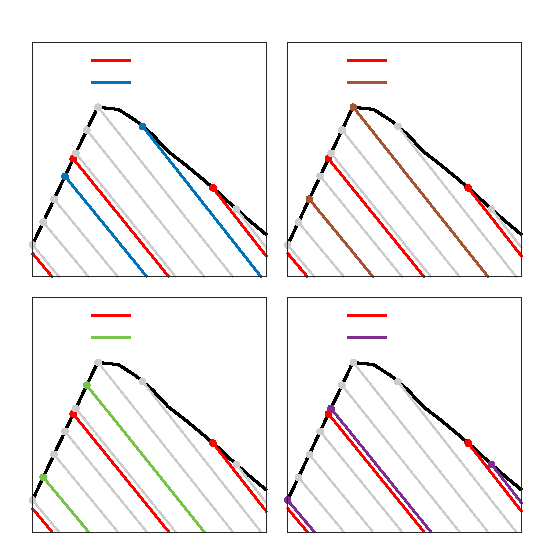
\includegraphics{./figures/parts/02/chapters/04/sections/02/correct_oversampling}}%
    \gplfronttext
  \end{picture}%
\endgroup

  \caption{\small Μεγέθυνση της μη γραμμικής περιοχής που περικλείεται με
           κόκκινο χρώμα στο σχήμα \ref{fig:02_02:the_problem}. Οι κόκκινες
           γραμμές υποδηλώνουν ακτίνες της πραγματικής σάρωσης $\mathcal{S}_R$.
           Οι μπλε, καφέ, πράσινες, και μωβ γραμμές υποδηλώνουν
           ακτίνες $2^\nu = 2^2$ διακριτών εικονικών σαρώσεων που λαμβάνονται
           από την εκτίμηση στάσης $\hat{\bm{p}}(x,y,\hat{\theta})$ σε
           $\gamma/2^\nu$, $\nu = 2$ γωνιακά βήματα, ξεκινώντας από τον
           εκτιμώμενο προσανατολισμό του αισθητήρα $\hat{\theta}$. Η εικονική
           σάρωση που συμβολίζεται με μωβ χρώμα σημειώνει την υψηλότερη τιμή
           της μετρικής Ποσοστού Διάκρισης (PD) μεταξύ όλων των $2^\nu$
           εικονικών σαρώσεων. Χρησιμοποιώντας τη μετρική PD και επιλέγοντας
           την εκτίμηση προσανατολισμού που αντιστοιχεί στην εικονική σάρωση με
           τη μέγιστη τιμή PD, το σφάλμα εκτίμησης προσανατολισμού φράσσεται
           εγγυημένα άνωθεν από την τιμή $\gamma/2^{\nu+1}$ στην περίπτωση
           όπου οι μετρήσεις του φυσικού αισθητήρα δεν διαταράσσονται από
           θόρυβο και ο χάρτης αναπαριστά το περιβάλλον τέλεια}
  \label{fig:oversampling_correct}
\end{figure}

Αντί της κατασκευής μίας εικονικής σάρωσης $2^\nu N_s$ ακτίνων, και της
εκτέλεσης διόρθωσης του προσανατολισμού μία φορά (Παρατήρηση
\ref{rem:sizes_incorrect}), το βέλτιστο σφάλμα προσανατολισμού $|\phi| \in
[0,\gamma / 2^{1+\nu}]$ για έναν δεδομένο ρυθμό δειγματοληψίας $\mu = 2^\nu$
και διακριτική γωνία $\gamma$ μπορεί να επιτευχθεί με τον υπολογισμό
$2^\nu$ εικονικών σαρώσεων μεγέθους $N_s$, εκτελώντας διόρθωση προσανατολισμού
$2^\nu$ φορές. Η διόρθωση προσανατολισμού πραγματοποιείται μία φορά μεταξύ της
ανόθευτης πραγματικής σάρωσης και της εικονικής σάρωσης $\mathcal{S}_V^k$, η
οποία λαμβάνεται από τη στάση $\hat{\bm{p}}(x,y,\hat{\theta}_k)$:
\begin{align}
  \hat{\theta}_k = \hat{\theta} + k \cdot \gamma / 2^\nu, \ \ \ k = 0,\dots,2^\nu-1 \label{eq:theta_k_theseus}
\end{align}
για συνολικά $2^\nu$ φορές, με αποτέλεσμα $2^\nu$ εκτιμήσεις προσανατολισμού.

Όσο αφορά στις μεθόδους Fourier-Mellin μίας διάστασης και τη μέθοδο του
Προκρούστη, η μετρική ευθυγράμμισης μεταξύ της $k$-οστής εικονικής σάρωσης και
της πραγματικής σάρωσης υπολογίζεται σύμφωνα το Ποσοστό Διάκρισης (Percent
Discrimination---PD). Η μετρική του Ποσοστού Διάκρισης για την $k$-οστή
εικονική σάρωση PD$_k$ $\in [0,1]$, και είναι ανάλογη του βαθμού ευθυγράμμισης
μεταξύ των σαρώσεων $\mathcal{S}_R$ και $\mathcal{S}_V^k$ για όλες τις $2^\nu$
σαρώσεις $\mathcal{S}_V^k$. Το Ποσοστό Διάκρισης ανάμεσα στην πραγματική
μέτρηση $\mathcal{S}_R$ και την εικονική σάρωση $\mathcal{S}_V^k$ ορίζεται ως:
\begin{align}
  \text{PD}_k = \dfrac{2 \ \Phi(\Psi,\Omega_k)}{\Phi(\Psi,\Psi) + \Phi(\Omega_k,\Omega_k)} \label{eq:pd}
\end{align}

Για τη μεν περίπτωση της μεθόδου Fourier-Mellin: $\Phi = \max q$, όπου $q =
\mathcal{F}^{-1}\{Q\}$, με τον όρο $Q$ να ορίζεται από την εξίσωση
(\ref{eq:Q0}) με ορίσματα τα διανύσματα σαρώσεων εισόδου $\Psi = \mathcal{S}_R$
και $\Omega_k = \mathcal{S}_V^k$.

Για τη δε περίπτωση της μεθόδου του Προκρούστη: $\Phi = T$, όπου $T$ είναι το
μέγιστο ίχνος με ορίσματα τους πίνακες $\Psi = \bm{P}_R$ και $\Omega_k =
\bm{P}_{V_k}$ (Επακόλουθο \ref{corollary:umeyama}). Εδώ το σύνολο σημείων
$\bm{P}_R$ κατέχει τις συντεταγμένες των τελικών σημείων των ακτίνων της
πραγματικής σάρωσης $\mathcal{S}_R$ προβεβλημμένες στο επίπεδο $x-y$ από την
αρχή $\bm{O}(0,0,0)$ όπως προηγουμένως, και το σύνολο $\bm{P}_{V_k}$ κατέχει
τις συντεταγμένες των τελικών σημείων της $k$-οστής εικονικής σάρωσης, επίσης
προβεβλημμένες στο επίπεδο $x-y$ από το $\bm{O}$.

Όσο αφορά στη μέθοδο Πρώτων Αρχών η σύγκριση ανάμεσα στις σαρώσεις
$\mathcal{S}_R$ και $\mathcal{S}_V^k$ δεν είναι δόκιμη, καθώς αυτή αποτελεί
μέθοδο συνεχούς χώρου, και συνεπώς δεν ορίζεται μετρική ευθυγράμμισης. \\

Έστω τώρα ότι $k_{\max} \in \mathbb{Z}_{\geq 0} : k_{\max} \in [0,2^{\nu-1}]$
συμβολίζει το δείκτη της $k$-οστής εικονικής σάρωσης $\mathcal{S}_V^{k_{\max}}$
που σημειώνει τον υψηλότερο δείκτη ευθυγράμμισης PD$_k$:
$\text{PD}_{k_{\max}} = \max \{\text{PD}_k\}$. Έστω επίσης $I \in \mathbb{Z}$
το ακέραιο πολλαπλάσιο κατά το οποίο εάν πολλαπλασιαστεί η διακριτική γωνία
$\gamma$ τότε η σάρωση $\mathcal{S}_V^{k_{\max}}$ ευθυγραμμίζεται με την
$\mathcal{S}_R$ με τρόπο τέτοιο που παράγεται η μετρική ευθυγράμμισης
PD$_{k_{\max}}$. Τότε εάν η εκτίμηση προσανατολισμού του αισθητήρα ενημερωθεί
σε
\begin{align}
  \hat{\theta}^\prime = \hat{\theta} + I \cdot \gamma + k_{\max} \cdot \dfrac{\gamma}{2^\nu}
\end{align}
το επίλοιπο σφάλμα εκτίμησης προσανατολισμού $\phi$ φράσσεται από:
\begin{align}
  |\phi| = \mod(|\theta - \hat{\theta}^\prime|, \gamma) \leq \dfrac{\gamma}{2^{1+\nu}} < \dfrac{\gamma}{2}
  \label{eq:phi_theseus}
\end{align}
για $\nu \in \mathbb{Z}_{>0}$.

Ο στόχος (\ref{objective:02_04}) επιτυγχάνεται με τη μέθοδο που εισαγάγαμε σε
αυτή την ενότητα για τη μέθοδο Fourier-Mellin μίας διάστασης (ενότητα
\ref{subsection:02_04_02:01}) και τη μέθοδο του Προκρούστη (ενότητα
\ref{subsection:02_04_02:03}) υπό τις προϋποθέσεις ότι (α)
$\bm{l} = \hat{\bm{l}}$, (β) το αρχικό σφάλμα προσανατολισμού είναι
$|\theta - \hat{\theta}| > \gamma / 2^{1+\nu}$ για δεδομένο βαθμό
δειγματοληψίας $\nu$, (γ) οι μετρήσεις του φυσικού αισθητήρα δεν διαταράσσονται
από θόρυβο, και (δ) ο χάρτης του περιβάλλοντος το αναπαριστά τέλεια.

Στο σχήμα \ref{fig:02_04_02:theseus} απεικονίζονται οι ίδιες αρχικές συνθήκες
με αυτές της διαμόρφωσης του σχήματος \ref{fig:02_04_02:sinis}. Η ευθυγράμμιση
προσανατολισμού εκτελείται και πάλι διαδοχικά για βαθμούς δειγματοληψίας του
χάρτη $\bm{M}$ $(\nu_{\min}, \nu_{\max}) = (0,3)$, αλλά αυτή τη φορά το σφάλμα
εκτίμησης προσανατολισμού $\phi^{(\nu)}$ φράσσεται στο τέλος κάθε βήματος
δειγματοληψίας $\nu$ από την ποσότητα $\dfrac{\gamma}{2^{1+\nu}}$. Στο σχήμα
\ref{fig:02_04_02:theseus_exec_times} απεικονίζεται ο μέσος χρόνος εκτέλεσης
της μεθόδου Fourier-Mellin μίας διάστασης με χρήση της επιπρόσθετης μεθόδου
του Θησέα για αυξανόμενο αριθμό ακτίνων $N_s$ με βάση την ίδια διαμόρφωση.

Στο σχήμα \ref{fig:02_04_02:theseus_pd} η άνω σειρά απεικονίζει τα πραγματικά
δεδομένα Ποσοστών Διάκρισης και επίλοιπων σφαλμάτων των υποψήφιων
προσανατολισμών ανά βαθμό δειγματοληψίας, τα οποία παρήχθησαν κατά την εφαρμογή
της μεθόδου Θησέα επί των μεθόδων γωνιακής ευθυγράμμισης Fourier-Mellin και
Προκρούστη που παρουσιάζονται στην εικόνα \ref{fig:02_04_02:theseus}. Στην
αριστερή πλευρά της κάτω σειράς απεικονίζεται σχηματικά η εξέλιξη της ημίσειας
κατάτμησης του επίλοιπου σφάλματος προσανατολισμού ανά βαθμό δειγματοληψίας,
και στη δεξιά το Ποσοστό Διάκρισης που αντιστοιχεί σε κάθε σφάλμα.
Συγκεκριμένα, με γκρι χρώμα σημειώνεται η μετρική που εμφανίζει τη μέγιστη τιμή
ανάμεσα σε όλες εκείνες του ίδιου βαθμού δειγματοληψίας.  Αντιπαραβάλλοντας
αυτές με τα δεδομένα της δεξιάς στήλης της άνω σειράς και στη συνέχεια αυτά με
εκείνα της αριστερής στήλης της ίδιας σειράς παρατηρούμε ότι τα ελάχιστα
επίλοιπα σφάλματα εμφανίζουν τα μέγιστα ποσοστά διάκρισης, σε συνέπεια με την
εξίσωση (\ref{eq:phi_theseus}) και την ανάλυση της παρούσας ενότητας.

\begin{figure}[h]\centering
  \vspace{1.0cm}
  \definecolor{sr}{RGB}{43,131,186}
\definecolor{svi}{RGB}{215,25, 28}
\definecolor{svf}{RGB}{179,143,59}
\definecolor{g}{RGB}{0,178,93}
\definecolor{k}{RGB}{0,0,0}
\definecolor{m}{RGB}{255,0,255}

% GNUPLOT: LaTeX picture with Postscript
\begingroup
  \makeatletter
  \providecommand\color[2][]{%
    \GenericError{(gnuplot) \space\space\space\@spaces}{%
      Package color not loaded in conjunction with
      terminal option `colourtext'%
    }{See the gnuplot documentation for explanation.%
    }{Either use 'blacktext' in gnuplot or load the package
      color.sty in LaTeX.}%
    \renewcommand\color[2][]{}%
  }%
  \providecommand\includegraphics[2][]{%
    \GenericError{(gnuplot) \space\space\space\@spaces}{%
      Package graphicx or graphics not loaded%
    }{See the gnuplot documentation for explanation.%
    }{The gnuplot epslatex terminal needs graphicx.sty or graphics.sty.}%
    \renewcommand\includegraphics[2][]{}%
  }%
  \providecommand\rotatebox[2]{#2}%
  \@ifundefined{ifGPcolor}{%
    \newif\ifGPcolor
    \GPcolorfalse
  }{}%
  \@ifundefined{ifGPblacktext}{%
    \newif\ifGPblacktext
    \GPblacktexttrue
  }{}%
  % define a \g@addto@macro without @ in the name:
  \let\gplgaddtomacro\g@addto@macro
  % define empty templates for all commands taking text:
  \gdef\gplbacktext{}%
  \gdef\gplfronttext{}%
  \makeatother
  \ifGPblacktext
    % no textcolor at all
    \def\colorrgb#1{}%
    \def\colorgray#1{}%
  \else
    % gray or color?
    \ifGPcolor
      \def\colorrgb#1{\color[rgb]{#1}}%
      \def\colorgray#1{\color[gray]{#1}}%
      \expandafter\def\csname LTw\endcsname{\color{white}}%
      \expandafter\def\csname LTb\endcsname{\color{black}}%
      \expandafter\def\csname LTa\endcsname{\color{black}}%
      \expandafter\def\csname LT0\endcsname{\color[rgb]{1,0,0}}%
      \expandafter\def\csname LT1\endcsname{\color[rgb]{0,1,0}}%
      \expandafter\def\csname LT2\endcsname{\color[rgb]{0,0,1}}%
      \expandafter\def\csname LT3\endcsname{\color[rgb]{1,0,1}}%
      \expandafter\def\csname LT4\endcsname{\color[rgb]{0,1,1}}%
      \expandafter\def\csname LT5\endcsname{\color[rgb]{1,1,0}}%
      \expandafter\def\csname LT6\endcsname{\color[rgb]{0,0,0}}%
      \expandafter\def\csname LT7\endcsname{\color[rgb]{1,0.3,0}}%
      \expandafter\def\csname LT8\endcsname{\color[rgb]{0.5,0.5,0.5}}%
    \else
      % gray
      \def\colorrgb#1{\color{black}}%
      \def\colorgray#1{\color[gray]{#1}}%
      \expandafter\def\csname LTw\endcsname{\color{white}}%
      \expandafter\def\csname LTb\endcsname{\color{black}}%
      \expandafter\def\csname LTa\endcsname{\color{black}}%
      \expandafter\def\csname LT0\endcsname{\color{black}}%
      \expandafter\def\csname LT1\endcsname{\color{black}}%
      \expandafter\def\csname LT2\endcsname{\color{black}}%
      \expandafter\def\csname LT3\endcsname{\color{black}}%
      \expandafter\def\csname LT4\endcsname{\color{black}}%
      \expandafter\def\csname LT5\endcsname{\color{black}}%
      \expandafter\def\csname LT6\endcsname{\color{black}}%
      \expandafter\def\csname LT7\endcsname{\color{black}}%
      \expandafter\def\csname LT8\endcsname{\color{black}}%
    \fi
  \fi
    \setlength{\unitlength}{0.0500bp}%
    \ifx\gptboxheight\undefined%
      \newlength{\gptboxheight}%
      \newlength{\gptboxwidth}%
      \newsavebox{\gptboxtext}%
    \fi%
    \setlength{\fboxrule}{0.5pt}%
    \setlength{\fboxsep}{1pt}%
\begin{picture}(8000.00,8000.00)%
    \gplgaddtomacro\gplbacktext{%
    }%
    \gplgaddtomacro\gplfronttext{%
    }%
    \gplgaddtomacro\gplbacktext{%
      \colorrgb{0.15,0.15,0.15}%
      \put(4868,4400){\makebox(0,0)[r]{\strut{}$2^{-5}$}}%
      \colorrgb{0.15,0.15,0.15}%
      \put(4868,4633){\makebox(0,0)[r]{\strut{}$2^{-4}$}}%
      \colorrgb{0.15,0.15,0.15}%
      \put(4868,4867){\makebox(0,0)[r]{\strut{}$2^{-3}$}}%
      \colorrgb{0.15,0.15,0.15}%
      \put(4868,5100){\makebox(0,0)[r]{\strut{}$2^{-2}$}}%
      \colorrgb{0.15,0.15,0.15}%
      \put(4868,5334){\makebox(0,0)[r]{\strut{}$2^{-1}$}}%
      \colorrgb{0.15,0.15,0.15}%
      \put(4868,5567){\makebox(0,0)[r]{\strut{}$2^{0}$}}%
      \colorrgb{0.15,0.15,0.15}%
      \put(4868,5801){\makebox(0,0)[r]{\strut{}$2^{1}$}}%
      \colorrgb{0.15,0.15,0.15}%
      \put(4868,6034){\makebox(0,0)[r]{\strut{}$2^{2}$}}%
      \colorrgb{0.15,0.15,0.15}%
      \put(4868,6268){\makebox(0,0)[r]{\strut{}$2^{3}$}}%
      \colorrgb{0.15,0.15,0.15}%
      \put(4868,6501){\makebox(0,0)[r]{\strut{}$2^{4}$}}%
      \colorrgb{0.15,0.15,0.15}%
      \put(4868,6735){\makebox(0,0)[r]{\strut{}$2^{5}$}}%
      \colorrgb{0.15,0.15,0.15}%
      \put(4868,6968){\makebox(0,0)[r]{\strut{}$2^{6}$}}%
      \colorrgb{0.15,0.15,0.15}%
      \put(4868,7202){\makebox(0,0)[r]{\strut{}$2^{7}$}}%
      \colorrgb{0.15,0.15,0.15}%
      \put(5900,4180){\makebox(0,0){\strut{}$3$}}%
      \colorrgb{0.15,0.15,0.15}%
      \put(6199,4180){\makebox(0,0){\strut{}$4$}}%
      \colorrgb{0.15,0.15,0.15}%
      \put(6499,4180){\makebox(0,0){\strut{}$5$}}%
      \colorrgb{0.15,0.15,0.15}%
      \put(6799,4180){\makebox(0,0){\strut{}$6$}}%
    }%
    \gplgaddtomacro\gplfronttext{%
    }%
    \gplgaddtomacro\gplbacktext{%
    }%
    \gplgaddtomacro\gplfronttext{%
    }%
    \gplgaddtomacro\gplbacktext{%
      \colorrgb{0.15,0.15,0.15}%
      \put(4868,800){\makebox(0,0)[r]{\strut{}$2^{-5}$}}%
      \colorrgb{0.15,0.15,0.15}%
      \put(4868,1033){\makebox(0,0)[r]{\strut{}$2^{-4}$}}%
      \colorrgb{0.15,0.15,0.15}%
      \put(4868,1267){\makebox(0,0)[r]{\strut{}$2^{-3}$}}%
      \colorrgb{0.15,0.15,0.15}%
      \put(4868,1500){\makebox(0,0)[r]{\strut{}$2^{-2}$}}%
      \colorrgb{0.15,0.15,0.15}%
      \put(4868,1734){\makebox(0,0)[r]{\strut{}$2^{-1}$}}%
      \colorrgb{0.15,0.15,0.15}%
      \put(4868,1967){\makebox(0,0)[r]{\strut{}$2^{0}$}}%
      \colorrgb{0.15,0.15,0.15}%
      \put(4868,2201){\makebox(0,0)[r]{\strut{}$2^{1}$}}%
      \colorrgb{0.15,0.15,0.15}%
      \put(4868,2434){\makebox(0,0)[r]{\strut{}$2^{2}$}}%
      \colorrgb{0.15,0.15,0.15}%
      \put(4868,2668){\makebox(0,0)[r]{\strut{}$2^{3}$}}%
      \colorrgb{0.15,0.15,0.15}%
      \put(4868,2901){\makebox(0,0)[r]{\strut{}$2^{4}$}}%
      \colorrgb{0.15,0.15,0.15}%
      \put(4868,3135){\makebox(0,0)[r]{\strut{}$2^{5}$}}%
      \colorrgb{0.15,0.15,0.15}%
      \put(4868,3368){\makebox(0,0)[r]{\strut{}$2^{6}$}}%
      \colorrgb{0.15,0.15,0.15}%
      \put(4868,3602){\makebox(0,0)[r]{\strut{}$2^{7}$}}%
      \colorrgb{0.15,0.15,0.15}%
      \put(5900,580){\makebox(0,0){\strut{}$3$}}%
      \colorrgb{0.15,0.15,0.15}%
      \put(6199,580){\makebox(0,0){\strut{}$4$}}%
      \colorrgb{0.15,0.15,0.15}%
      \put(6499,580){\makebox(0,0){\strut{}$5$}}%
      \colorrgb{0.15,0.15,0.15}%
      \put(6799,580){\makebox(0,0){\strut{}$6$}}%
    }%
    \gplgaddtomacro\gplfronttext{%
      \colorrgb{0.15,0.15,0.15}
      \put(5900,7900){\makebox(0,0){\strut{}{\color{k}{\rule[0.6mm]{0.5cm}{0.5mm}}} $\dfrac{|\theta-\hat{\theta}[k]|}{\gamma}$}}%
      \put(5400,7519){\makebox(0,0){\strut{}{\color{g}{\rule[0.6mm]{0.5cm}{0.5mm}}} $2^{-1}$}}%
      \put(6400,7519){\makebox(0,0){\strut{}{\color{m}{\rule[0.6mm]{0.5cm}{0.5mm}}} $2^{-4}$}}%

      \put(1100,7519){\makebox(0,0){\strut{}{\color{k}{\rule[0.6mm]{0.5cm}{0.5mm}}} $\bm{M}$}}%
      \put(1850,7519){\makebox(0,0){\strut{}{\color{sr}{\rule[0.6mm]{0.5cm}{0.5mm}}} $\bm{p}$}}%
      \put(2600,7519){\makebox(0,0){\strut{}{\color{svi}{\rule[0.6mm]{0.5cm}{0.5mm}}} $\hat{\bm{p}}[0]$}}%
      \put(3600,7519){\makebox(0,0){\strut{}{\color{svf}{\rule[0.6mm]{0.5cm}{0.5mm}}} $\hat{\bm{p}}[k_{6}]$}}%

      \put(5100,3869){\makebox(0,0){\strut{}$\nu$}}%
      \put(5400,3869){\makebox(0,0){\strut{}\fcolorbox{black}{sinisn0}{\rule{0pt}{6pt}\rule{6pt}{0pt} 0}}} %
      \put(5800,3869){\makebox(0,0){\strut{}\fcolorbox{black}{sinisn1}{\rule{0pt}{6pt}\rule{6pt}{0pt} 1}}} %
      \put(6200,3869){\makebox(0,0){\strut{}\fcolorbox{black}{sinisn2}{\rule{0pt}{6pt}\rule{6pt}{0pt} 2}}} %
      \put(6600,3869){\makebox(0,0){\strut{}\fcolorbox{black}{sinisn3}{\rule{0pt}{6pt}\rule{6pt}{0pt} 3}}} %

      \put(2300,4039){\makebox(0,0){\strut{} \texttt{rc\_fm}}}%
      \put(2300,250){\makebox(0,0){\strut{} \texttt{rc\_uf}}}%

      \put(5899,250){\makebox(0,0){\strut{}Αριθμός επαναλήψεων $k$}}%
    }
    \gplbacktext
    \put(0,0){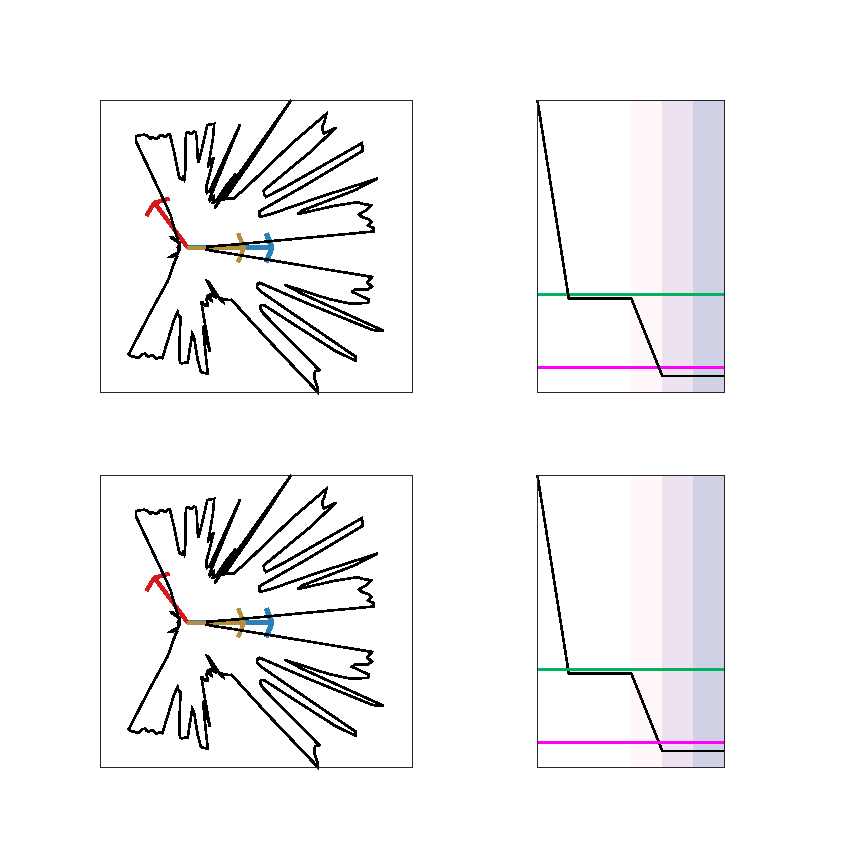
\includegraphics{./figures/parts/02/chapters/04/sections/02/theseus}}%
    \gplfronttext
  \end{picture}%
\endgroup

  \vspace{0.5cm}
  \caption{\small Η ορθή προσέγγιση ελάττωσης του γωνιακού σφάλματος εκτίμησης
           της μεθόδου Θησέα για διαδοχική υπερδειγματοληψία βαθμών
           $(\nu_{\min}, \nu_{\max}) = (0,3)$. Το σφάλμα εκτίμησης
           προσανατολισμού $\phi^{(\nu)}$ των δύο μεθόδων φράσσεται στο τέλος
           κάθε βήματος δειγματοληψίας $\nu$ από την ποσότητα
           $\gamma/2^{1+\nu}$}
  \label{fig:02_04_02:theseus}
\end{figure}

\begin{figure}[h]\centering
  % GNUPLOT: LaTeX picture with Postscript
\begingroup
  \makeatletter
  \providecommand\color[2][]{%
    \GenericError{(gnuplot) \space\space\space\@spaces}{%
      Package color not loaded in conjunction with
      terminal option `colourtext'%
    }{See the gnuplot documentation for explanation.%
    }{Either use 'blacktext' in gnuplot or load the package
      color.sty in LaTeX.}%
    \renewcommand\color[2][]{}%
  }%
  \providecommand\includegraphics[2][]{%
    \GenericError{(gnuplot) \space\space\space\@spaces}{%
      Package graphicx or graphics not loaded%
    }{See the gnuplot documentation for explanation.%
    }{The gnuplot epslatex terminal needs graphicx.sty or graphics.sty.}%
    \renewcommand\includegraphics[2][]{}%
  }%
  \providecommand\rotatebox[2]{#2}%
  \@ifundefined{ifGPcolor}{%
    \newif\ifGPcolor
    \GPcolorfalse
  }{}%
  \@ifundefined{ifGPblacktext}{%
    \newif\ifGPblacktext
    \GPblacktexttrue
  }{}%
  % define a \g@addto@macro without @ in the name:
  \let\gplgaddtomacro\g@addto@macro
  % define empty templates for all commands taking text:
  \gdef\gplfronttext{}%
  \gdef\gplfronttext{}%
  \makeatother
  \ifGPblacktext
    % no textcolor at all
    \def\colorrgb#1{}%
    \def\colorgray#1{}%
  \else
    % gray or color?
    \ifGPcolor
      \def\colorrgb#1{\color[rgb]{#1}}%
      \def\colorgray#1{\color[gray]{#1}}%
      \expandafter\def\csname LTw\endcsname{\color{white}}%
      \expandafter\def\csname LTb\endcsname{\color{black}}%
      \expandafter\def\csname LTa\endcsname{\color{black}}%
      \expandafter\def\csname LT0\endcsname{\color[rgb]{1,0,0}}%
      \expandafter\def\csname LT1\endcsname{\color[rgb]{0,1,0}}%
      \expandafter\def\csname LT2\endcsname{\color[rgb]{0,0,1}}%
      \expandafter\def\csname LT3\endcsname{\color[rgb]{1,0,1}}%
      \expandafter\def\csname LT4\endcsname{\color[rgb]{0,1,1}}%
      \expandafter\def\csname LT5\endcsname{\color[rgb]{1,1,0}}%
      \expandafter\def\csname LT6\endcsname{\color[rgb]{0,0,0}}%
      \expandafter\def\csname LT7\endcsname{\color[rgb]{1,0.3,0}}%
      \expandafter\def\csname LT8\endcsname{\color[rgb]{0.5,0.5,0.5}}%
    \else
      % gray
      \def\colorrgb#1{\color{black}}%
      \def\colorgray#1{\color[gray]{#1}}%
      \expandafter\def\csname LTw\endcsname{\color{white}}%
      \expandafter\def\csname LTb\endcsname{\color{black}}%
      \expandafter\def\csname LTa\endcsname{\color{black}}%
      \expandafter\def\csname LT0\endcsname{\color{black}}%
      \expandafter\def\csname LT1\endcsname{\color{black}}%
      \expandafter\def\csname LT2\endcsname{\color{black}}%
      \expandafter\def\csname LT3\endcsname{\color{black}}%
      \expandafter\def\csname LT4\endcsname{\color{black}}%
      \expandafter\def\csname LT5\endcsname{\color{black}}%
      \expandafter\def\csname LT6\endcsname{\color{black}}%
      \expandafter\def\csname LT7\endcsname{\color{black}}%
      \expandafter\def\csname LT8\endcsname{\color{black}}%
    \fi
  \fi
    \setlength{\unitlength}{0.0500bp}%
    \ifx\gptboxheight\undefined%
      \newlength{\gptboxheight}%
      \newlength{\gptboxwidth}%
      \newsavebox{\gptboxtext}%
    \fi%
    \setlength{\fboxrule}{0.5pt}%
    \setlength{\fboxsep}{1pt}%
\begin{picture}(4800.00,3600.00)%
    \gplgaddtomacro\gplfronttext{%
      \colorrgb{0.15,0.15,0.15}%
      \put(1078,704){\makebox(0,0)[r]{\strut{}$0.0$}}%
      \colorrgb{0.15,0.15,0.15}%
      \put(1078,1175){\makebox(0,0)[r]{\strut{}$20.0$}}%
      \colorrgb{0.15,0.15,0.15}%
      \put(1078,1646){\makebox(0,0)[r]{\strut{}$40.0$}}%
      \colorrgb{0.15,0.15,0.15}%
      \put(1078,2117){\makebox(0,0)[r]{\strut{}$60.0$}}%
      \colorrgb{0.15,0.15,0.15}%
      \put(1078,2588){\makebox(0,0)[r]{\strut{}$80.0$}}%
      \colorrgb{0.15,0.15,0.15}%
      \put(1078,3059){\makebox(0,0)[r]{\strut{}$100.0$}}%
      \colorrgb{0.15,0.15,0.15}%
      \put(1210,484){\makebox(0,0){\strut{}$360$$\cdot$$2^0$}}%
      \colorrgb{0.15,0.15,0.15}%
      \put(2231,484){\makebox(0,0){\strut{}$360$$\cdot$$2^1$}}%
      \colorrgb{0.15,0.15,0.15}%
      \put(3251,484){\makebox(0,0){\strut{}$360$$\cdot$$2^2$}}%
      \colorrgb{0.15,0.15,0.15}%
      \put(4272,484){\makebox(0,0){\strut{}$360$$\cdot$$2^3$}}%
    }%
    \gplgaddtomacro\gplfronttext{%
      \colorrgb{0.15,0.15,0.15}%
      \put(176,1881){\rotatebox{90}{\makebox(0,0){\strut{}Χρόνος εκτέλεσης [ms]}}}%
      \colorrgb{0.15,0.15,0.15}%
      \put(2741,154){\makebox(0,0){\strut{}Αριθμός ακτίνων $N_s$}}%
      \colorrgb{0.00,0.00,0.00}%
      \put(2741,3269){\makebox(0,0){\strut{}$T_{\texttt{rc\_fm}\ \circ \ \texttt{DBH}}$}}%
    }%
    \put(0,0){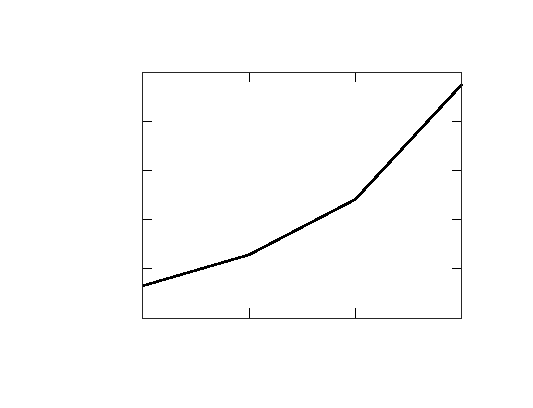
\includegraphics{./figures/parts/02/chapters/04/sections/02/times_rc_fm_DBH}}%
    \gplfronttext
  \end{picture}%
\endgroup

  \caption{\small Μέσος χρόνος εκτέλεσης της μεθόδου Fourier-Mellin μίας
           διάστασης με χρήση της μεθόδου του Θησέα για
           $(\nu_{\min}, \nu_{\max}) = (0,3)$, για αυξανόμενο αριθμό ακτίνων
           $N_s$}
  \label{fig:02_04_02:theseus_exec_times}
\end{figure}

\begin{figure}[h]\centering
  \begin{subfigure}{0.5\linewidth}
    \setlength{\DTbaselineskip}{20pt}
    \dirtree{%
    .1 $|\phi^{(0)}|   / \dfrac{\gamma}{2^0}=$  \textcolor{k}{0.45} $< 2^{-1}$.
    .2 $|\phi_0^{(1)}| / \dfrac{\gamma}{2^1}=$  \textcolor{mygray}{0.45}.
    .2 $|\phi_1^{(1)}| / \dfrac{\gamma}{2^1}=$  \textcolor{k}{0.22} $< 2^{-1}$.
    .3 $|\phi_0^{(2)}| / \dfrac{\gamma}{2^2}=$  \textcolor{k}{0.19} $< 2^{-1}$.
    .4 $|\phi_0^{(3)}| / \dfrac{\gamma}{2^3}=$  \textcolor{k}{0.39} $< 2^{-1}$.
    .4 $|\phi_1^{(3)}| / \dfrac{\gamma}{2^3}=$  \textcolor{mygray}{1.39}.
    .4 $|\phi_2^{(3)}| / \dfrac{\gamma}{2^3}=$  \textcolor{mygray}{2.39}.
    .4 $|\phi_3^{(3)}| / \dfrac{\gamma}{2^3}=$  \textcolor{mygray}{3.39}.
    .4 $|\phi_4^{(3)}| / \dfrac{\gamma}{2^3}=$  \textcolor{mygray}{3.60}.
    .4 $|\phi_5^{(3)}| / \dfrac{\gamma}{2^3}=$  \textcolor{mygray}{2.60}.
    .4 $|\phi_6^{(3)}| / \dfrac{\gamma}{2^3}=$  \textcolor{mygray}{1.60}.
    .4 $|\phi_7^{(3)}| / \dfrac{\gamma}{2^3}=$  \textcolor{mygray}{0.60}.
    .3 $|\phi_1^{(2)}| / \dfrac{\gamma}{2^2}=$  \textcolor{mygray}{1.195}.
    .3 $|\phi_2^{(2)}| / \dfrac{\gamma}{2^2}=$  \textcolor{mygray}{1.80}.
    .3 $|\phi_3^{(2)}| / \dfrac{\gamma}{2^2}=$  \textcolor{mygray}{0.80}.
    }
  \end{subfigure}%
  \begin{subfigure}{0.45\linewidth}\vspace{-0.1cm}
    \setlength{\DTbaselineskip}{22.5pt}
    \dirtree{%
    .1 $\text{PD}^{(0)}   =$ \textcolor{k}{0.99101}.
    .2 $\text{PD}_0^{(1)} =$ \textcolor{mygray}{0.99101}.
    .2 $\text{PD}_1^{(1)} =$ \textcolor{k}{0.99986} $\geq \text{PD}_\ast^{(1)}$.
    .3 $\text{PD}_0^{(2)} =$ \textcolor{k}{0.99986} $\geq \text{PD}_\ast^{(2)}$.
    .4 $\text{PD}_0^{(3)} =$ \textcolor{k}{0.99986} $\geq \text{PD}_\ast^{(3)}$.
    .4 $\text{PD}_1^{(3)} =$ \textcolor{mygray}{0.99721}.
    .4 $\text{PD}_2^{(3)} =$ \textcolor{mygray}{0.98130}.
    .4 $\text{PD}_3^{(3)} =$ \textcolor{mygray}{0.98516}.
    .4 $\text{PD}_4^{(3)} =$ \textcolor{mygray}{0.99101}.
    .4 $\text{PD}_5^{(3)} =$ \textcolor{mygray}{0.99575}.
    .4 $\text{PD}_6^{(3)} =$ \textcolor{mygray}{0.99835}.
    .4 $\text{PD}_7^{(3)} =$ \textcolor{mygray}{0.99973}.
    .3 $\text{PD}_1^{(2)} =$ \textcolor{mygray}{0.98130}.
    .3 $\text{PD}_2^{(2)} =$ \textcolor{mygray}{0.99101}.
    .3 $\text{PD}_3^{(2)} =$ \textcolor{mygray}{0.99835}.
    }
  \end{subfigure}\vspace{0.5cm}
  \begin{subfigure}{0.5\linewidth}
    \begin{onion}{1.0cm}
      \annulus[sinisn0]{0}{0}{360}[$\phi^{(0)}$]
      \annulus[sinisn1]{1}{0}{180}[$\phi_0^{(1)}$]
      \annulus[sinisn1]{1}{180}{360}[$\phi_1^{(1)}$]
      \annulus[sinisn2]{2}{180}{225}[$\phi_0^{(2)}$]
      \annulus[sinisn2]{2}{225}{270}[$\phi_1^{(2)}$]
      \annulus[sinisn2]{2}{270}{315}[$\phi_2^{(2)}$]
      \annulus[sinisn2]{2}{315}{360}[$\phi_3^{(2)}$]
      \annulus[sinisn3]{3}{180}{185.625}
      \annulus[sinisn3]{3}{185.625}{191.25}
      \annulus[sinisn3]{3}{191.25}{196.875}
      \annulus[sinisn3]{3}{196.875}{202.5}
      \annulus[sinisn3]{3}{202.5}{208.125}
      \annulus[sinisn3]{3}{208.125}{213.75}
      \annulus[sinisn3]{3}{213.75}{219.375}
      \annulus[sinisn3]{3}{219.375}{225}
    \end{onion}
  \end{subfigure}%
  \begin{subfigure}{0.5\linewidth}\vspace{-0.1cm}
    \begin{onion}{1.0cm}
      \annulus[sinisn0]{0}{0}{360}[PD$^{(0)}$]
      \annulus[sinisn0]{1}{0}{180}[PD$_0^{(1)}$]
      \annulus[litegray]{1}{180}{360}[PD$_1^{(1)}$]
      \annulus[litegray]{2}{180}{225}[PD$_0^{(2)}$]
      \annulus[sinisn0]{2}{225}{270}[PD$_1^{(2)}$]
      \annulus[sinisn0]{2}{270}{315}[PD$_2^{(2)}$]
      \annulus[sinisn0]{2}{315}{360}[PD$_3^{(2)}$]
      \annulus[litegray]{3}{180}{185.625}
      \annulus[sinisn0]{3}{185.625}{191.25}
      \annulus[sinisn0]{3}{191.25}{196.875}
      \annulus[sinisn0]{3}{196.875}{202.5}
      \annulus[sinisn0]{3}{202.5}{208.125}
      \annulus[sinisn0]{3}{208.125}{213.75}
      \annulus[sinisn0]{3}{213.75}{219.375}
      \annulus[sinisn0]{3}{219.375}{225}
    \end{onion}
  \end{subfigure}
\vspace{-1cm}
\caption{\small Τα πραγματικά δεδομένα Ποσοστών Διάκρισης
         $\texttt{PD}^{(\nu)}_{0:2^{\nu}-1}$ και επίλοιπων σφαλμάτων
         $\phi^{(\nu)}_{0:2^{\nu}-1}$ των υποψήφιων προσανατολισμών που αφορούν
         στα επίπεδα δειγματοληψίας $\nu$, τα οποία προέκυψαν κατά την εφαρμογή
         της μεθόδου Θησέα επί των μεθόδων γωνιακής ευθυγράμμισης
         Fourier-Mellin και Προκρούστη που παρουσιάζονται στην εικόνα
         \ref{fig:02_04_02:theseus}. Η κάτω σειρά απεικονίζει σχηματικά: στα
         αριστερά την αναδρομική εξέλιξη της κατάτμησης του αρχικού επίλοιπου
         σφάλματος $\phi^{(0)}$ σε ημίσεια σφάλματα, και στα δεξιά τα
         αντιστοιχούντα μέγιστα ποσοστά διάκρισης ανά βαθμό δειγματοληψίας.
         Παρατηρήστε πως υπάρχει ευθεία αντιστοιχία του μέγιστου ποσοστού
         διάκρισης (γκρι) με το ελάχιστο επίλοιπο σφάλμα προσανατολισμού}
\label{fig:02_04_02:theseus_pd}
\end{figure}

Ο Αλγόριθμος \ref{alg:theseus} παρουσιάζει τη μέθοδο διόρθωσης προσανατολισμού
που προτείνουμε σε μορφή ψευδοκώδικα, για ορίσματα $\texttt{rc} =
\{\texttt{rc\_fm}, \texttt{rc\_uf}\}$ (Αλγόριθμοι \ref{alg:algorithm_fmrc} και
\ref{alg:algorithm_ufrc}).

\begin{algorithm}[h]
  \caption{\texttt{rc\_theseus}}
  \begin{spacing}{1.5}
  \begin{algorithmic}[1]
    \REQUIRE \texttt{rc}, $\bm{M}$, $\mathcal{S}_R$, $\hat{\bm{p}}(x, y, \hat{\theta})$, $\gamma$, $N_s$, $\nu$
    \ENSURE $\hat{\theta}^\prime$
    \STATE $(\hat{\bm{\Theta}}, \textbf{PD}) \leftarrow \texttt{rc\_theseus\_core}(\texttt{rc}, \bm{M}, \mathcal{S}_R, \hat{\bm{p}}(x, y, \hat{\theta}), \gamma, N_s, \nu)$
    \STATE $k_{\max} \leftarrow \arg\max\textbf{PD}$
    \STATE $\hat{\theta}^\prime \leftarrow \hat{\bm{\Theta}}[k_{\max}]$
    \RETURN $\hat{\theta}^\prime$
  \end{algorithmic}
  \end{spacing}
  \label{alg:theseus}
\end{algorithm}

\begin{algorithm}[h]
  \caption{\texttt{rc\_theseus\_core}}
  \begin{spacing}{1.5}
  \begin{algorithmic}[1]
    \REQUIRE \texttt{rc}, $\bm{M}$, $\mathcal{S}_R$, $\hat{\bm{p}}(x, y, \hat{\theta})$, $\gamma$, $N_s$, $\nu$
    \ENSURE $\hat{\bm{\Theta}}$, $\textbf{PD}$
    \STATE $\hat{\bm{\Theta}}, \textbf{PD} \leftarrow \{\varnothing\}$
    \FOR{$k = 0 : 2^\nu-1$}
      \STATE $\hat{\bm{p}}_k \leftarrow (x, y, \hat{\theta} + k \cdot \gamma/2^\nu)$
      \STATE $\mathcal{S}_V^k \leftarrow \texttt{scan\_map}(\bm{M}, \hat{\bm{p}}_k, N_s)$
      \STATE $(\hat{\theta}^\prime, w_k) \leftarrow \texttt{rc}(\mathcal{S}_R, \mathcal{S}_V, \hat{\bm{p}}_k, \gamma)$
      \STATE $\texttt{append} \ \ \hat{\theta}_k = \hat{\theta}^\prime + k \cdot \gamma/2^\nu$ to $\hat{\bm{\Theta}}$
      \STATE $(\cdot,w_k^{R}) \leftarrow \texttt{rc}(\mathcal{S}_R, \mathcal{S}_R, \hat{\bm{p}}_k, \gamma)$
      \STATE $(\cdot,w_k^{V}) \leftarrow \texttt{rc}(\mathcal{S}_V^k, \mathcal{S}_V^k, \hat{\bm{p}}_k, \gamma)$
      \STATE $\texttt{append} \ \ \dfrac{2w_k}{w_k^{R} + w_k^{V}}$ to \textbf{PD}
      \STATE $k \leftarrow k + 1$
    \ENDFOR
    \RETURN $(\hat{\bm{\Theta}}, \textbf{PD})$
  \end{algorithmic}
  \end{spacing}
  \label{alg:core_theseus}
\end{algorithm}

\begin{algorithm}[h]
  \caption{\texttt{scan\_map}}
  \begin{spacing}{1.3}
    \begin{algorithmic}[1]
      \REQUIRE $\bm{M}, \bm{p}(x, y, \theta), N_s$
      \ENSURE $\mathcal{S}_V$
      \STATE $\mathcal{S}_V \leftarrow \{\varnothing\}$
      \FOR{$n = 0:N_s-1$}
      \STATE $\lambda_n \leftarrow -\pi + \dfrac{2\pi}{N_s} n$
      \STATE $\theta_n \leftarrow \lambda_n + \hat{\theta}$
      \STATE $(x_n,y_n) \leftarrow \texttt{intersect}(\bm{M}, (x,y, \theta_n))$
      \STATE $d_n \leftarrow \|(x- x_n, y-y_n)\|_2$
      \STATE \texttt{append} $(d_n, \lambda_n)$ to $\mathcal{S}_V$
      \ENDFOR
      \RETURN $\mathcal{S}_V$
    \end{algorithmic}
  \end{spacing}
  \label{alg:scan_map}
\end{algorithm}


%%%%%%%%%%%%%%%%%%%%%%%%%%%%%%%%%%%%%%%%%%%%%%%%%%%%%%%%%%%%%%%%%%%%%%%%%%%%%%%%
\section{Μεθοδολογία εκτίμησης}
  \label{section:02_03_03}
  Έστω τώρα το αντίστροφο ως προς την προηγούμενη ενότητα πρόβλημα:
έστω ότι η πραγματική και η εκτιμώμενη στάση είναι ίσες ως προς τον
προσανατολισμό $\hat{\theta} = \theta$, αλλά άνισες ως προς τη θέση
$\hat{\bm{l}} \neq \bm{l}$.

%%%%%%%%%%%%%%%%%%%%%%%%%%%%%%%%%%%%%%%%%%%%%%%%%%%%%%%%%%%%%%%%%%%%%%%%%%%%%%%%
\subsection{Η μέθοδος Πρώτων Αρχών}
\label{subsection:02_04_03:01}

Εάν ο χάρτης αναπαριστά το περιβάλλον τέλεια και ο φυσικός αισθητήρας αναφέρει
μετρήσεις χωρίς διαταραχές, τότε η εκτίμηση της θέσης του αισθητήρα μπορεί να
οδηγηθεί αυθαίρετα κοντά στην πραγματική θέση. Σε πραγματικές συνθήκες, όταν οι
ακτίνες των πραγματικών σαρώσεων ή/και των εικονικών σαρώσεων αλλοιώνονται από
προσθετικό θόρυβο πεπερασμένου μέγιστου μέτρου, η εκτίμηση θέσης μπορεί να
φραχθεί σε μια γειτονιά της πραγματικής θέσης του αισθητήρα. Το Θεώρημα
\ref{prop:theorem_without_disturbance} τυποποιεί αυτή τη δήλωση
\cite{Filotheou2022d}.

\begin{bw_box}
\begin{theorem}
  \label{prop:theorem_without_disturbance}
  Έστω ότι ισχύουν οι υποθέσεις του Προβλήματος \ref{prob:02_04}, και ότι
  $\hat{\theta} = \theta$. Έστω επίσης ότι η εικονική σάρωση $\mathcal{S}_V$ που
  συλλαμβάνεται από τη στάση $\hat{\bm{p}}$ εντός του χάρτη $\bm{M}$
  συμβολίζεται με $\mathcal{S}_V|_{\bm{\hat{p}}}$. Έστω ακόμα ότι οι
  δισδιάστατες σαρώσεις $\mathcal{S}_R$ και $\mathcal{S}_V$ είναι απαλλαγμένες
  από διαταραχές, δηλαδή ότι οι αποστάσεις που καταγράφουν οι ακτίνες της
  πραγματικής σάρωσης προς τα γύρω του εμπόδια αντιστοιχούν στις πραγματικές
  αποστάσεις του αισθητήρα από τα εν λόγω εμπόδια, και ότι ο χάρτης του
  περιβάλλοντος το αναπαριστά τέλεια. Αντιμετωπίζοντας την
  εκτίμηση της θέσης του αισθητήρα ως μεταβλητή κατάστασης
  $\hat{\bm{l}}[k] = [\hat{x}[k], \hat{y}[k]]^\top$ και ενημερώνοντάς την
  σύμφωνα με την εξίσωση διαφορών
  \begin{align}
    \hat{\bm{l}}[k+1] = \hat{\bm{l}}[k] + \bm{u}[k]
    \label{eq:difference_equation_without_disturbance}
  \end{align}
  όπου $\hat{\bm{l}}[0] = \hat{\bm{l}} = [\hat{x}, \hat{y}]^{\top}$,
  (δηλαδή η παρεχόμενη αρχική εκτίμηση της θέσης), $\bm{u}$ είναι ένα διάνυσμα
  διαστάσεων $2 \times 1$ που στο εξής θα αναφέρεται ως
  \textit{διάνυσμα ελέγχου}:
  \begin{align}
    \bm{u}[k] = \dfrac{1}{N_s}
    \begin{bmatrix}
      \cos\hat{\theta} & \sin\hat{\theta} \\\
      \sin\hat{\theta} & - \cos\hat{\theta}
    \end{bmatrix}
    \begin{bmatrix}
      X_{1,r}\big(\mathcal{S}_R, \mathcal{S}_V|_{\bm{\hat{p}}[k]}\big) \vspace{0.2cm} \\
      X_{1,i}\big(\mathcal{S}_R, \mathcal{S}_V|_{\bm{\hat{p}}[k]}\big)
    \end{bmatrix}
    \label{eq:control_vector_without_disturbance}
  \end{align}
  όπου $X_{1,r}(\cdot)$ και $X_{1,i}(\cdot)$ είναι, αντίστοιχα, το πραγματικό
  και φανταστικό μέρος της μιγαδικής ποσότητας $X_1$:
  \begin{align}
    X_1\big(\mathcal{S}_R, \mathcal{S}_V|_{\bm{\hat{p}}[k]}\big) &= X_{1,r}\big(\mathcal{S}_R, \mathcal{S}_V|_{\bm{\hat{p}}[k]}\big)
      + i \cdot X_{1,i}\big(\mathcal{S}_R, \mathcal{S}_V|_{\bm{\hat{p}}[k]}\big) \nonumber \\
      &= \sum\limits_{n=0}^{N_s-1}(\mathcal{S}_R[n] - \mathcal{S}_V[n]|_{\bm{\hat{p}}[k]}) \cdot e^{-i \frac{2 \pi n}{N_s}} \label{eq:X1}
  \end{align}
  όπου $\mathcal{S}_R[n]$ και $\mathcal{S}_V[n]|_{\bm{\hat{p}}[k]}$ είναι,
  αντίστοιχα, οι αναφερόμενες αποστάσεις της $n$-οστής ακτίνας της πραγματικής
  $\mathcal{S}_R$ και εικονικής σάρωσης $\mathcal{S}_V|_{\bm{\hat{p}}[k]}$, και
  $\hat{\bm{p}}[k] = (\hat{\bm{l}}[k], \hat{\theta})$---τότε η εκτίμηση θέσης
  $\hat{\bm{l}}[k]$ \textit{συγκλίνει ομοιόμορφα ασυμπτωτικά στην πραγματική
  θέση} $\bm{l}$ \textit{καθώς} $k \rightarrow \infty$.
\end{theorem}
\end{bw_box}

\begin{corollary}
  Μια λύση που ικανοποιεί το στόχο (\ref{objective:02_04}) είναι αυστηρά
  εγγυημένη για κάθε αρχική θέση $\hat{\bm{l}}[0]$ στην περίπτωση που οι
  μετρήσεις του φυσικού αισθητήρα δεν φέρουν διαταραχές και ο χάρτης $\bm{M}$
  δεν είναι διεφθαρμένος ως προς το περιβάλλον που αναπαριστά.
\end{corollary}

Στην πράξη το σύστημα ελέγχου
(\ref{eq:difference_equation_without_disturbance},
\ref{eq:control_vector_without_disturbance}) αφήνεται να επαναληφθεί είτε
έως ότου το μέτρο του διανύσματος ελέγχου $\bm{u}[k]$ φτάσει σε ένα επαρκώς
μικρό μέγεθος $\|\bm{u}[k]\|_2 < \varepsilon_u$, όπου $\varepsilon_u$ είναι
επαρκώς μικρό---π.χ. $\varepsilon_u < 10^{-3}$---ή για $I_T > 0$ επαναλήψεις
(ένα αρκετά μεγάλο, εξωτερικά παρεχόμενο όριο μέγιστων επαναλήψεων---π.χ. $I_T
\geq 20$). Επομένως, συμβολίζοντας με $k_{stop} \in (0, I_T]$ τον δείκτη
της τελευταίας επανάληψης, και με
$\hat{\bm{l}}^{\prime} = \hat{\bm{l}}[k_{stop}]$ τότε
$\|\bm{e}(\bm{l}, \hat{\bm{l}}^{\prime})\|_2 < \|\bm{e}(\bm{l}, \hat{\bm{l}}[0])\|_2$,
και επομένως ο στόχος (\ref{objective:02_04}) ικανοποιείται.

Στο σχήμα \ref{fig:02_04_03:map_convergence} απεικονίζονται οι τροχιές της
εκτίμησης θέσης βάσει εφαρμογής του Θεωρήματος
\ref{prop:theorem_without_disturbance} για έναν αισθητήρα $N_s = 360$ ακτίνων,
με θέση $\bm{l} = (0.83, -0.98)$ [m] και αρχική εκτίμηση θέσης $\hat{\bm{l}} =
(4.0,-4.0)$ [m]. Οι ακτίνες της πραγματικής σάρωσης $\mathcal{S}_R$ και των
εικονικών σαρώσεων $\mathcal{S}_V$ διαταράσσονται από θόρυβο κανονικά
κατανεμημένο με μηδενική μέση τιμή και τυπική απόκλιση $\sigma_R$ και
$\sigma_V$ αντίστοιχα. Η άνω σειρά απεικονίζει τις τροχιές εκτίμησης για
τυπικές αποκλίσεις $\sigma_R = \sigma_V = 0.0$ m, και η κάτω σειρά για
$\sigma_R = \sigma_V = 0.05$ m.

\begin{figure}[!h]\centering\vspace{1cm}
  % GNUPLOT: LaTeX picture with Postscript
\begingroup
  \makeatletter
  \providecommand\color[2][]{%
    \GenericError{(gnuplot) \space\space\space\@spaces}{%
      Package color not loaded in conjunction with
      terminal option `colourtext'%
    }{See the gnuplot documentation for explanation.%
    }{Either use 'blacktext' in gnuplot or load the package
      color.sty in LaTeX.}%
    \renewcommand\color[2][]{}%
  }%
  \providecommand\includegraphics[2][]{%
    \GenericError{(gnuplot) \space\space\space\@spaces}{%
      Package graphicx or graphics not loaded%
    }{See the gnuplot documentation for explanation.%
    }{The gnuplot epslatex terminal needs graphicx.sty or graphics.sty.}%
    \renewcommand\includegraphics[2][]{}%
  }%
  \providecommand\rotatebox[2]{#2}%
  \@ifundefined{ifGPcolor}{%
    \newif\ifGPcolor
    \GPcolorfalse
  }{}%
  \@ifundefined{ifGPblacktext}{%
    \newif\ifGPblacktext
    \GPblacktexttrue
  }{}%
  % define a \g@addto@macro without @ in the name:
  \let\gplgaddtomacro\g@addto@macro
  % define empty templates for all commands taking text:
  \gdef\gplbacktext{}%
  \gdef\gplfronttext{}%
  \makeatother
  \ifGPblacktext
    % no textcolor at all
    \def\colorrgb#1{}%
    \def\colorgray#1{}%
  \else
    % gray or color?
    \ifGPcolor
      \def\colorrgb#1{\color[rgb]{#1}}%
      \def\colorgray#1{\color[gray]{#1}}%
      \expandafter\def\csname LTw\endcsname{\color{white}}%
      \expandafter\def\csname LTb\endcsname{\color{black}}%
      \expandafter\def\csname LTa\endcsname{\color{black}}%
      \expandafter\def\csname LT0\endcsname{\color[rgb]{1,0,0}}%
      \expandafter\def\csname LT1\endcsname{\color[rgb]{0,1,0}}%
      \expandafter\def\csname LT2\endcsname{\color[rgb]{0,0,1}}%
      \expandafter\def\csname LT3\endcsname{\color[rgb]{1,0,1}}%
      \expandafter\def\csname LT4\endcsname{\color[rgb]{0,1,1}}%
      \expandafter\def\csname LT5\endcsname{\color[rgb]{1,1,0}}%
      \expandafter\def\csname LT6\endcsname{\color[rgb]{0,0,0}}%
      \expandafter\def\csname LT7\endcsname{\color[rgb]{1,0.3,0}}%
      \expandafter\def\csname LT8\endcsname{\color[rgb]{0.5,0.5,0.5}}%
    \else
      % gray
      \def\colorrgb#1{\color{black}}%
      \def\colorgray#1{\color[gray]{#1}}%
      \expandafter\def\csname LTw\endcsname{\color{white}}%
      \expandafter\def\csname LTb\endcsname{\color{black}}%
      \expandafter\def\csname LTa\endcsname{\color{black}}%
      \expandafter\def\csname LT0\endcsname{\color{black}}%
      \expandafter\def\csname LT1\endcsname{\color{black}}%
      \expandafter\def\csname LT2\endcsname{\color{black}}%
      \expandafter\def\csname LT3\endcsname{\color{black}}%
      \expandafter\def\csname LT4\endcsname{\color{black}}%
      \expandafter\def\csname LT5\endcsname{\color{black}}%
      \expandafter\def\csname LT6\endcsname{\color{black}}%
      \expandafter\def\csname LT7\endcsname{\color{black}}%
      \expandafter\def\csname LT8\endcsname{\color{black}}%
    \fi
  \fi
    \setlength{\unitlength}{0.0500bp}%
    \ifx\gptboxheight\undefined%
      \newlength{\gptboxheight}%
      \newlength{\gptboxwidth}%
      \newsavebox{\gptboxtext}%
    \fi%
    \setlength{\fboxrule}{0.5pt}%
    \setlength{\fboxsep}{1pt}%
\begin{picture}(9000.00,6000.00)%
    \gplgaddtomacro\gplbacktext{%
      \colorrgb{0.15,0.15,0.15}%
      \put(768,3408){\makebox(0,0)[r]{\strut{}$-5.0$}}%
      \colorrgb{0.15,0.15,0.15}%
      \put(768,3732){\makebox(0,0)[r]{\strut{}$-4.0$}}%
      \colorrgb{0.15,0.15,0.15}%
      \put(768,4055){\makebox(0,0)[r]{\strut{}$-3.0$}}%
      \colorrgb{0.15,0.15,0.15}%
      \put(768,4379){\makebox(0,0)[r]{\strut{}$-2.0$}}%
      \colorrgb{0.15,0.15,0.15}%
      \put(768,4703){\makebox(0,0)[r]{\strut{}$-1.0$}}%
      \colorrgb{0.15,0.15,0.15}%
      \put(768,5026){\makebox(0,0)[r]{\strut{}$0.0$}}%
      \colorrgb{0.15,0.15,0.15}%
      \put(768,5350){\makebox(0,0)[r]{\strut{}$1.0$}}%
      \colorrgb{0.15,0.15,0.15}%
      \put(1046,3188){\makebox(0,0){\strut{}$-3.0$}}%
      \colorrgb{0.15,0.15,0.15}%
      \put(1693,3188){\makebox(0,0){\strut{}$-1.0$}}%
      \colorrgb{0.15,0.15,0.15}%
      \put(2340,3188){\makebox(0,0){\strut{}$1.0$}}%
      \colorrgb{0.15,0.15,0.15}%
      \put(2988,3188){\makebox(0,0){\strut{}$3.0$}}%
      \colorrgb{0.15,0.15,0.15}%
      \put(3635,3188){\makebox(0,0){\strut{}$5.0$}}%
    }%
    \gplgaddtomacro\gplfronttext{%
      \colorrgb{0.15,0.15,0.15}%
      \put(-2,4379){\rotatebox{90}{\makebox(0,0){\strut{}$y$ [m]}}}%
    }%
    \gplgaddtomacro\gplbacktext{%
      \colorrgb{0.15,0.15,0.15}%
      \put(4908,3360){\makebox(0,0)[r]{\strut{}$-1.01$}}%
      \colorrgb{0.15,0.15,0.15}%
      \put(4908,3870){\makebox(0,0)[r]{\strut{}$-1.0$}}%
      \colorrgb{0.15,0.15,0.15}%
      \put(4908,4380){\makebox(0,0)[r]{\strut{}$-0.99$}}%
      \colorrgb{0.15,0.15,0.15}%
      \put(4908,4889){\makebox(0,0)[r]{\strut{}$-0.98$}}%
      \colorrgb{0.15,0.15,0.15}%
      \put(4908,5399){\makebox(0,0)[r]{\strut{}$-0.97$}}%
      \colorrgb{0.15,0.15,0.15}%
      \put(5040,3140){\makebox(0,0){\strut{}$0.81$}}%
      \colorrgb{0.15,0.15,0.15}%
      %\put(5550,3140){\makebox(0,0){\strut{}$0.82$}}%
      \colorrgb{0.15,0.15,0.15}%
      \put(6060,3140){\makebox(0,0){\strut{}$0.83$}}%
      \colorrgb{0.15,0.15,0.15}%
      %\put(6569,3140){\makebox(0,0){\strut{}$0.84$}}%
      \colorrgb{0.15,0.15,0.15}%
      \put(7079,3140){\makebox(0,0){\strut{}$0.85$}}%
      \colorrgb{0.15,0.15,0.15}%
      %\put(7589,3140){\makebox(0,0){\strut{}$0.86$}}%
      \colorrgb{0.15,0.15,0.15}%
      \put(8099,3140){\makebox(0,0){\strut{}$0.87$}}%
    }%
    \gplgaddtomacro\gplfronttext{%
    }%
    \gplgaddtomacro\gplbacktext{%
      \colorrgb{0.15,0.15,0.15}%
      \put(768,648){\makebox(0,0)[r]{\strut{}$-5.0$}}%
      \colorrgb{0.15,0.15,0.15}%
      \put(768,972){\makebox(0,0)[r]{\strut{}$-4.0$}}%
      \colorrgb{0.15,0.15,0.15}%
      \put(768,1295){\makebox(0,0)[r]{\strut{}$-3.0$}}%
      \colorrgb{0.15,0.15,0.15}%
      \put(768,1619){\makebox(0,0)[r]{\strut{}$-2.0$}}%
      \colorrgb{0.15,0.15,0.15}%
      \put(768,1943){\makebox(0,0)[r]{\strut{}$-1.0$}}%
      \colorrgb{0.15,0.15,0.15}%
      \put(768,2266){\makebox(0,0)[r]{\strut{}$0.0$}}%
      \colorrgb{0.15,0.15,0.15}%
      \put(768,2590){\makebox(0,0)[r]{\strut{}$1.0$}}%
      \colorrgb{0.15,0.15,0.15}%
      \put(1046,428){\makebox(0,0){\strut{}$-3.0$}}%
      \colorrgb{0.15,0.15,0.15}%
      \put(1693,428){\makebox(0,0){\strut{}$-1.0$}}%
      \colorrgb{0.15,0.15,0.15}%
      \put(2340,428){\makebox(0,0){\strut{}$1.0$}}%
      \colorrgb{0.15,0.15,0.15}%
      \put(2988,428){\makebox(0,0){\strut{}$3.0$}}%
      \colorrgb{0.15,0.15,0.15}%
      \put(3635,428){\makebox(0,0){\strut{}$5.0$}}%
    }%
    \gplgaddtomacro\gplfronttext{%
      \colorrgb{0.15,0.15,0.15}%
      \put(-2,1619){\rotatebox{90}{\makebox(0,0){\strut{}$y$ [m]}}}%
      \colorrgb{0.15,0.15,0.15}%
      \put(2429,98){\makebox(0,0){\strut{}$x$ [m]}}%
    }%
    \gplgaddtomacro\gplbacktext{%
      \colorrgb{0.15,0.15,0.15}%
      \put(4908,600){\makebox(0,0)[r]{\strut{}$-1.01$}}%
      \colorrgb{0.15,0.15,0.15}%
      \put(4908,1110){\makebox(0,0)[r]{\strut{}$-1.0$}}%
      \colorrgb{0.15,0.15,0.15}%
      \put(4908,1620){\makebox(0,0)[r]{\strut{}$-0.99$}}%
      \colorrgb{0.15,0.15,0.15}%
      \put(4908,2129){\makebox(0,0)[r]{\strut{}$-0.98$}}%
      \colorrgb{0.15,0.15,0.15}%
      \put(4908,2639){\makebox(0,0)[r]{\strut{}$-0.97$}}%
      \colorrgb{0.15,0.15,0.15}%
      \put(5040,380){\makebox(0,0){\strut{}$0.81$}}%
      \colorrgb{0.15,0.15,0.15}%
      %\put(5550,380){\makebox(0,0){\strut{}$0.82$}}%
      \colorrgb{0.15,0.15,0.15}%
      \put(6060,380){\makebox(0,0){\strut{}$0.83$}}%
      \colorrgb{0.15,0.15,0.15}%
      %\put(6569,380){\makebox(0,0){\strut{}$0.84$}}%
      \colorrgb{0.15,0.15,0.15}%
      \put(7079,380){\makebox(0,0){\strut{}$0.85$}}%
      \colorrgb{0.15,0.15,0.15}%
      %\put(7589,380){\makebox(0,0){\strut{}$0.86$}}%
      \colorrgb{0.15,0.15,0.15}%
      \put(8099,380){\makebox(0,0){\strut{}$0.87$}}%
      \put(1800,6100){\makebox(0,0){\strut{}{$\circ$ \small Αρχική εκτίμηση θέσης $\hat{\bm{l}}[0]$}}}
      \put(4500,6100){\makebox(0,0){\strut{}{$\bulletmagenta$ \small Πραγματική θέση $\bm{l}$}}}
      \put(7000,6100){\makebox(0,0){\strut{}{$\bulletblack$ \small Εκτιμώμενη θέση $\hat{\bm{l}}[k]$}}}
      \put(2400,5600){\makebox(0,0){\strut{}Πλήρης άποψη}}
      \put(6600,5600){\makebox(0,0){\strut{}Εστιασμένη άποψη}}
    }%
    \gplgaddtomacro\gplfronttext{%
      \colorrgb{0.15,0.15,0.15}%
      \put(6569,50){\makebox(0,0){\strut{}$x$ [m]}}%
    }%
    \gplbacktext
    \put(0,0){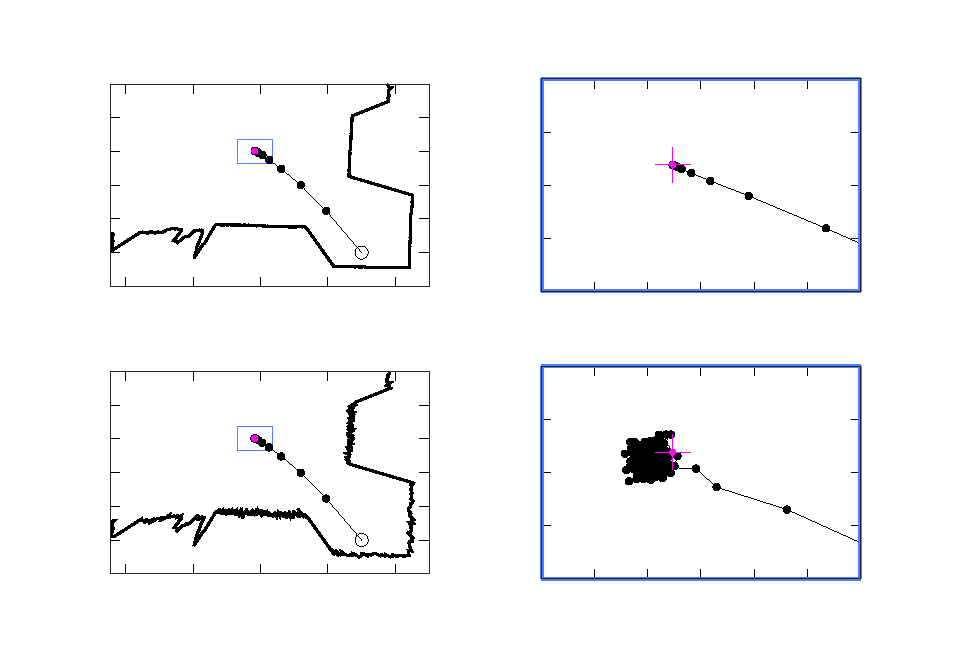
\includegraphics{./figures/parts/02/chapters/04/sections/03/translation_map_convergence}}%
    \gplfronttext
  \end{picture}%
\endgroup

\caption{\small Οι τροχιές της εκτίμησης θέσης βάσει εφαρμογής του Θεωρήματος
         \ref{prop:theorem_without_disturbance} για επίπεδο διαταραχών
         αποστάσεων $\sigma_R = \sigma_V = 0.0$ m (άνω σειρά) και
         $\sigma_R = \sigma_V = 0.05$ m (κάτω σειρά). Τα τελικά σφάλματα
         εκτίμησης θέσης είναι $2.04$e-$07$ m και $5.72$e-$03$ m αντίστοιχα.
         Η εκτίμηση θέσης συγκλίνει ομοιόμορφα ασυμπτωτικά στην πρώτη περίπτωση
         (Θεώρημα \ref{prop:theorem_without_disturbance}), ενώ στη δεύτερη
         είναι ομοιόμορφα φραγμένη σε μία γειτονιά της πραγματικής θέσης
         (Θεώρημα \ref{prop:theorem_with_disturbance})}
\label{fig:02_04_03:map_convergence}
\end{figure}

Το σχήμα \ref{fig:02_04_03:execution_times} απεικονίζει το μέσο χρόνο εκτέλεσης
μίας επανάληψης της μεθόδου διόρθωσης της εκτίμησης θέσης σε δέκα εκτελέσεις
για μέγιστο αριθμό εσωτερικών επαναλήψεων $I_T = 20$, για αυξανόμενο μέγεθος
σαρώσεων $N_s$. Ο αλγόριθμος \ref{alg:icte} παραθέτει σε ψευδοκώδικα τη μέθοδο
εκτίμησης της θέσης για δεδομένη και γνωστή εκτίμηση προσανατολισμού.

\begin{figure}[!h]\centering
  % GNUPLOT: LaTeX picture with Postscript
\begingroup
  \makeatletter
  \providecommand\color[2][]{%
    \GenericError{(gnuplot) \space\space\space\@spaces}{%
      Package color not loaded in conjunction with
      terminal option `colourtext'%
    }{See the gnuplot documentation for explanation.%
    }{Either use 'blacktext' in gnuplot or load the package
      color.sty in LaTeX.}%
    \renewcommand\color[2][]{}%
  }%
  \providecommand\includegraphics[2][]{%
    \GenericError{(gnuplot) \space\space\space\@spaces}{%
      Package graphicx or graphics not loaded%
    }{See the gnuplot documentation for explanation.%
    }{The gnuplot epslatex terminal needs graphicx.sty or graphics.sty.}%
    \renewcommand\includegraphics[2][]{}%
  }%
  \providecommand\rotatebox[2]{#2}%
  \@ifundefined{ifGPcolor}{%
    \newif\ifGPcolor
    \GPcolorfalse
  }{}%
  \@ifundefined{ifGPblacktext}{%
    \newif\ifGPblacktext
    \GPblacktexttrue
  }{}%
  % define a \g@addto@macro without @ in the name:
  \let\gplgaddtomacro\g@addto@macro
  % define empty templates for all commands taking text:
  \gdef\gplfronttext{}%
  \gdef\gplfronttext{}%
  \makeatother
  \ifGPblacktext
    % no textcolor at all
    \def\colorrgb#1{}%
    \def\colorgray#1{}%
  \else
    % gray or color?
    \ifGPcolor
      \def\colorrgb#1{\color[rgb]{#1}}%
      \def\colorgray#1{\color[gray]{#1}}%
      \expandafter\def\csname LTw\endcsname{\color{white}}%
      \expandafter\def\csname LTb\endcsname{\color{black}}%
      \expandafter\def\csname LTa\endcsname{\color{black}}%
      \expandafter\def\csname LT0\endcsname{\color[rgb]{1,0,0}}%
      \expandafter\def\csname LT1\endcsname{\color[rgb]{0,1,0}}%
      \expandafter\def\csname LT2\endcsname{\color[rgb]{0,0,1}}%
      \expandafter\def\csname LT3\endcsname{\color[rgb]{1,0,1}}%
      \expandafter\def\csname LT4\endcsname{\color[rgb]{0,1,1}}%
      \expandafter\def\csname LT5\endcsname{\color[rgb]{1,1,0}}%
      \expandafter\def\csname LT6\endcsname{\color[rgb]{0,0,0}}%
      \expandafter\def\csname LT7\endcsname{\color[rgb]{1,0.3,0}}%
      \expandafter\def\csname LT8\endcsname{\color[rgb]{0.5,0.5,0.5}}%
    \else
      % gray
      \def\colorrgb#1{\color{black}}%
      \def\colorgray#1{\color[gray]{#1}}%
      \expandafter\def\csname LTw\endcsname{\color{white}}%
      \expandafter\def\csname LTb\endcsname{\color{black}}%
      \expandafter\def\csname LTa\endcsname{\color{black}}%
      \expandafter\def\csname LT0\endcsname{\color{black}}%
      \expandafter\def\csname LT1\endcsname{\color{black}}%
      \expandafter\def\csname LT2\endcsname{\color{black}}%
      \expandafter\def\csname LT3\endcsname{\color{black}}%
      \expandafter\def\csname LT4\endcsname{\color{black}}%
      \expandafter\def\csname LT5\endcsname{\color{black}}%
      \expandafter\def\csname LT6\endcsname{\color{black}}%
      \expandafter\def\csname LT7\endcsname{\color{black}}%
      \expandafter\def\csname LT8\endcsname{\color{black}}%
    \fi
  \fi
    \setlength{\unitlength}{0.0500bp}%
    \ifx\gptboxheight\undefined%
      \newlength{\gptboxheight}%
      \newlength{\gptboxwidth}%
      \newsavebox{\gptboxtext}%
    \fi%
    \setlength{\fboxrule}{0.5pt}%
    \setlength{\fboxsep}{1pt}%
\begin{picture}(4800.00,3600.00)%
    \gplgaddtomacro\gplfronttext{%
      \colorrgb{0.15,0.15,0.15}%
      \put(946,704){\makebox(0,0)[r]{\strut{}$0.0$}}%
      \colorrgb{0.15,0.15,0.15}%
      \put(946,1175){\makebox(0,0)[r]{\strut{}$2.0$}}%
      \colorrgb{0.15,0.15,0.15}%
      \put(946,1646){\makebox(0,0)[r]{\strut{}$4.0$}}%
      \colorrgb{0.15,0.15,0.15}%
      \put(946,2117){\makebox(0,0)[r]{\strut{}$6.0$}}%
      \colorrgb{0.15,0.15,0.15}%
      \put(946,2588){\makebox(0,0)[r]{\strut{}$8.0$}}%
      \colorrgb{0.15,0.15,0.15}%
      \put(946,3059){\makebox(0,0)[r]{\strut{}$10.0$}}%
      \colorrgb{0.15,0.15,0.15}%
      \put(1078,484){\makebox(0,0){\strut{}$360$$\cdot$$2^0$}}%
      \colorrgb{0.15,0.15,0.15}%
      \put(2143,484){\makebox(0,0){\strut{}$360$$\cdot$$2^1$}}%
      \colorrgb{0.15,0.15,0.15}%
      \put(3207,484){\makebox(0,0){\strut{}$360$$\cdot$$2^2$}}%
      \colorrgb{0.15,0.15,0.15}%
      \put(4272,484){\makebox(0,0){\strut{}$360$$\cdot$$2^3$}}%
    }%
    \gplgaddtomacro\gplfronttext{%
      \colorrgb{0.15,0.15,0.15}%
      \put(176,1881){\rotatebox{90}{\makebox(0,0){\strut{}Χρόνος εκτέλεσης [ms]}}}%
      \colorrgb{0.15,0.15,0.15}%
      \put(2675,154){\makebox(0,0){\strut{}Αριθμός ακτίνων $N_s$}}%
      \colorrgb{0.00,0.00,0.00}%
      \put(2675,3269){\makebox(0,0){\strut{}$T_{\texttt{tc\_x1}}$}}%
    }%
    \put(0,0){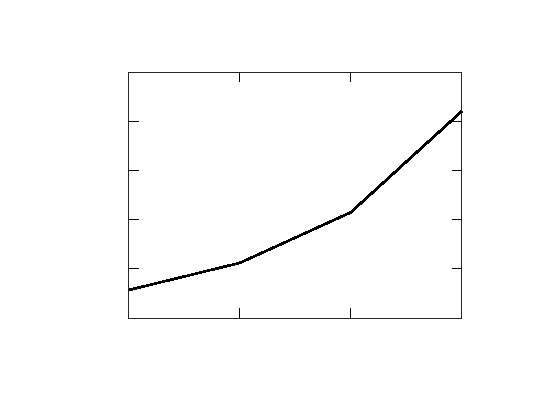
\includegraphics{./figures/parts/02/chapters/04/sections/03/translation_times_without_disturbance}}%
    \gplfronttext
  \end{picture}%
\endgroup

\caption{\small Ο μέσος χρόνος εκτέλεσης μίας επανάληψης της μεθόδου διόρθωσης
         της εκτίμησης θέσης για δέκα εκτελέσεις, ανά μέγεθος σαρώσεων εισόδου
         $N_s$}
\label{fig:02_04_03:execution_times}
\end{figure}

\begin{algorithm}[!h]
  \caption{\texttt{tc\_x1}}
  \begin{spacing}{1.4}
    \begin{algorithmic}[1]
      \REQUIRE $\bm{M}$, $\mathcal{S}_R$, $\hat{\bm{p}}(\hat{x}, \hat{y}, \hat{\theta})$, $k_{max}$, $\varepsilon_u$, $N_s$
      \ENSURE $\hat{\bm{p}}^\prime(\hat{x}^{\prime}, \hat{y}^{\prime}, \hat{\theta})$
      \STATE $k \leftarrow 0$
      \WHILE {$k < k_{max}$}
      \STATE $\mathcal{S}_V \leftarrow \texttt{scan\_map}(M, \hat{\bm{p}}, N_s)$
      \STATE $X_1 \leftarrow \texttt{diff\_dft}(\mathcal{S}_R, \mathcal{S}_V)$
      \STATE $(X_{1,r}, X_{1,i}) \leftarrow (\texttt{re}(X_1), \texttt{im}(X_1))$
      \STATE $\bm{u}_k = \begin{bmatrix}
              u_x \\ u_y
             \end{bmatrix}
             =
             \dfrac{1}{N_s}
             \begin{bmatrix}
               \cos\hat{\theta} & \sin\hat{\theta} \\
               \sin\hat{\theta} & -\cos\hat{\theta}
             \end{bmatrix}
             \begin{bmatrix}
               X_{1,r} \\ X_{1,i}
             \end{bmatrix}
             $
      \STATE $\hat{\bm{p}}\leftarrow \hat{\bm{p}}+ \bm{u}_k$
      \IF {$\|\bm{u}_k\|_2 < \varepsilon_u$}
        \STATE \texttt{break}
      \ENDIF
      \STATE $k \leftarrow k + 1$
      \ENDWHILE
      \STATE $\hat{\bm{p}}^\prime \leftarrow \hat{\bm{p}}$
      \RETURN $\hat{\bm{p}}^\prime$
    \end{algorithmic}
  \end{spacing}
  \label{alg:icte}
\end{algorithm}

\begin{algorithm}[!h]
  \caption{\texttt{diff\_dft}}
  \begin{spacing}{1.3}
    \begin{algorithmic}[1]
      \REQUIRE $\mathcal{S}_R, \mathcal{S}_V$
      \ENSURE $X_1$
      \STATE \texttt{assert} $|\mathcal{S}_R| = |\mathcal{S}_V|$
      \STATE $N_s \leftarrow |\mathcal{S}_R|$
      \STATE {$\bm{\Delta} \leftarrow \{\varnothing\}$}
      \FOR{$n = 0:N_s-1$}
      \STATE $d_n \leftarrow \mathcal{S}_R[n] - \mathcal{S}_V[n]$
      \STATE \texttt{append} $d$ to $\bm{\Delta}$
      \ENDFOR
      \STATE $\bm{X} \leftarrow \mathcal{F}\{\bm{\Delta}\}$
      \STATE $X_1 \leftarrow \bm{X}[1]$
      \RETURN $X_1$
    \end{algorithmic}
  \end{spacing}
  \label{alg:diff_dft}
\end{algorithm}


%%%%%%%%%%%%%%%%%%%%%%%%%%%%%%%%%%%%%%%%%%%%%%%%%%%%%%%%%%%%%%%%%%%%%%%%%%%%%%%%
\subsection{Ιδιότητες υπό γενικές συνθήκες}
\label{subsection:02_04_03:02}

Σε αντιστοιχία με τις μεθόδους ευθυγράμμισης προσανατολισμού, το σφάλμα θέσης
της μεθόδου ευθυγράμμισης θέσης Πρώτων Αρχών αυξάνει σε γενικές συνθήκες μη
σύμπτωσης της εκτίμησης προσανατολισμού με τον πραγματικό προσανατολισμό του
αισθητήρα, και σε συνθήκες διαταραχών των μετρήσεων του φυσικού αισθητήρα και
μη απολύτου σύμπτωσης του χάρτη με το περιβάλλον που αναπαριστά.

Σε πραγματικές συνθήκες, όταν οι ακτίνες των πραγματικών σαρώσεων ή/και των
εικονικών σαρώσεων αλλοιώνονται από προσθετικό θόρυβο πεπερασμένου μέγιστου
μέτρου, η εκτίμηση θέσης δεν είναι ικανή να προσεγγίσει ασυμπτώτικά την
πραγματική θέση με την εφαρμογή του Θεωρήματος
\ref{prop:theorem_without_disturbance}. Παρ' όλα αυτά, η εκτίμηση θέσης μπορεί
να φραχθεί σε μια γειτονιά της πραγματικής θέσης του αισθητήρα. Το Θεώρημα
\ref{prop:theorem_with_disturbance} τυποποιεί αυτή τη δήλωση
\cite{Filotheou2022d}.

\begin{bw_box}
\begin{theorem}
  \label{prop:theorem_with_disturbance}
  Έστω ότι ισχύουν οι υποθέσεις του Θεωρήματος
  \ref{prop:theorem_without_disturbance}. Έστω επιπλέον ότι η αποστάσεις που
  αναφέρονται από την πραγματική $\mathcal{S}_R$ και εικονική $\mathcal{S}_V$
  σάρωση επηρεάζονται από προσθετικές διαταραχές με πεπερασμένο μέγιστο μέτρο.
  Τότε η εκτίμηση θέσης $\hat{\bm{l}}[k]$ είναι ομοιόμορφα φραγμένη για $k \geq
  k_0$ και ομοιόμορφα τελικά φραγμένη σε μια γειτονιά της πραγματικής θέσης
  $\bm{l}$. Το μέγεθος της γειτονιάς εξαρτάται από τα δύο μέγιστα μέτρα
  (με την έννοια της infinity norm) των διαταραχών που αλλοιώνουν τις
  πραγματικές τιμές των δύο σαρώσεων.
\end{theorem}
\end{bw_box}

\begin{corollary}
  Σε σύγκριση με την περίπτωση που δεν υπάρχουν διαταραχές, μια λύση που
  ικανοποιεί το στόχο (\ref{objective:02_04}) δεν είναι αυστηρά εγγυημένη για
  κάθε αρχική θέση $\hat{\bm{l}}[0]$ στην περίπτωση που οι μετρήσεις του φυσικού
  αισθητήρα φέρουν διαταραχές ή/και ο χάρτης $\bm{M}$ είναι διεφθαρμένος ως προς
  το περιβάλλον που αναπαριστά.
\end{corollary}

Ας συμβολίσουμε και πάλι με $k_{stop} \in (0, I_T]$ τον δείκτη της τελευταίας
επανάληψης, με $\hat{\bm{l}}^{\prime} = \hat{\bm{l}}[k_{stop}]$ την τελική
εκτίμηση της θέσης του αισθητήρα, και με $B$ το τελικό φράγμα (ultimate bound)
του σφάλματος θέσης. Εάν $\|\bm{e}(\bm{l}, \hat{\bm{l}}[0])\|_2 > B$, το
Θεώρημα \ref{prop:theorem_with_disturbance} εγγυάται την ικανοποίηση του στόχου
(\ref{objective:02_04}) εάν $k_{stop} \geq k_0$. Εάν, από την άλλη πλευρά, εάν
$\|\bm{e}(\bm{l}, \hat{\bm{l}}[0])\|_2 \leq B$, δεν είναι βέβαιο ότι
$\|\bm{e}(\bm{l}, \hat{\bm{l}}^{\prime})\|_2 < \|\bm{e}(\bm{l},
\hat{\bm{l}}[0])\|_2$---αυτό που είναι βέβαιο σε αυτή την περίπτωση, όμως,
είναι ότι $\|\bm{e}(\bm{l}, \hat{\bm{l}}[k])\|_2 \ngtr B$ για όλα κάθε $k \geq
0$.

Επιπρόσθετα, σε γενικές συνθήκες δεν υφίσταται σύμπτωση της εκτίμησης
προσανατολισμού και του πραγματικού προσανατολισμού.  Το σχήμα
\ref{fig:02_04_03:tc_x1_non_convergence} απεικονίζει την εξέλιξη του μέτρου του
σφάλματος εκτίμησης θέσης για αυξανόμενες τιμές του σφάλματος εκτίμησης
προσανατολισμού $|\theta - \hat{\theta}|$ σε ένα πείραμα όπου το αρχικό σφάλμα
θέσης είναι $[-0.1165, 0.188]$ m.

\begin{figure}[!h]\centering
  \definecolor{a}{RGB}{244 224 127}
\definecolor{b}{RGB}{168 198 113}
\definecolor{c}{RGB}{96 168 109}
\definecolor{d}{RGB}{0 135 108}

% GNUPLOT: LaTeX picture with Postscript
\begingroup
  \makeatletter
  \providecommand\color[2][]{%
    \GenericError{(gnuplot) \space\space\space\@spaces}{%
      Package color not loaded in conjunction with
      terminal option `colourtext'%
    }{See the gnuplot documentation for explanation.%
    }{Either use 'blacktext' in gnuplot or load the package
      color.sty in LaTeX.}%
    \renewcommand\color[2][]{}%
  }%
  \providecommand\includegraphics[2][]{%
    \GenericError{(gnuplot) \space\space\space\@spaces}{%
      Package graphicx or graphics not loaded%
    }{See the gnuplot documentation for explanation.%
    }{The gnuplot epslatex terminal needs graphicx.sty or graphics.sty.}%
    \renewcommand\includegraphics[2][]{}%
  }%
  \providecommand\rotatebox[2]{#2}%
  \@ifundefined{ifGPcolor}{%
    \newif\ifGPcolor
    \GPcolorfalse
  }{}%
  \@ifundefined{ifGPblacktext}{%
    \newif\ifGPblacktext
    \GPblacktexttrue
  }{}%
  % define a \g@addto@macro without @ in the name:
  \let\gplgaddtomacro\g@addto@macro
  % define empty templates for all commands taking text:
  \gdef\gplfronttext{}%
  \gdef\gplfronttext{}%
  \makeatother
  \ifGPblacktext
    % no textcolor at all
    \def\colorrgb#1{}%
    \def\colorgray#1{}%
  \else
    % gray or color?
    \ifGPcolor
      \def\colorrgb#1{\color[rgb]{#1}}%
      \def\colorgray#1{\color[gray]{#1}}%
      \expandafter\def\csname LTw\endcsname{\color{white}}%
      \expandafter\def\csname LTb\endcsname{\color{black}}%
      \expandafter\def\csname LTa\endcsname{\color{black}}%
      \expandafter\def\csname LT0\endcsname{\color[rgb]{1,0,0}}%
      \expandafter\def\csname LT1\endcsname{\color[rgb]{0,1,0}}%
      \expandafter\def\csname LT2\endcsname{\color[rgb]{0,0,1}}%
      \expandafter\def\csname LT3\endcsname{\color[rgb]{1,0,1}}%
      \expandafter\def\csname LT4\endcsname{\color[rgb]{0,1,1}}%
      \expandafter\def\csname LT5\endcsname{\color[rgb]{1,1,0}}%
      \expandafter\def\csname LT6\endcsname{\color[rgb]{0,0,0}}%
      \expandafter\def\csname LT7\endcsname{\color[rgb]{1,0.3,0}}%
      \expandafter\def\csname LT8\endcsname{\color[rgb]{0.5,0.5,0.5}}%
    \else
      % gray
      \def\colorrgb#1{\color{black}}%
      \def\colorgray#1{\color[gray]{#1}}%
      \expandafter\def\csname LTw\endcsname{\color{white}}%
      \expandafter\def\csname LTb\endcsname{\color{black}}%
      \expandafter\def\csname LTa\endcsname{\color{black}}%
      \expandafter\def\csname LT0\endcsname{\color{black}}%
      \expandafter\def\csname LT1\endcsname{\color{black}}%
      \expandafter\def\csname LT2\endcsname{\color{black}}%
      \expandafter\def\csname LT3\endcsname{\color{black}}%
      \expandafter\def\csname LT4\endcsname{\color{black}}%
      \expandafter\def\csname LT5\endcsname{\color{black}}%
      \expandafter\def\csname LT6\endcsname{\color{black}}%
      \expandafter\def\csname LT7\endcsname{\color{black}}%
      \expandafter\def\csname LT8\endcsname{\color{black}}%
    \fi
  \fi
    \setlength{\unitlength}{0.0500bp}%
    \ifx\gptboxheight\undefined%
      \newlength{\gptboxheight}%
      \newlength{\gptboxwidth}%
      \newsavebox{\gptboxtext}%
    \fi%
    \setlength{\fboxrule}{0.5pt}%
    \setlength{\fboxsep}{1pt}%
\begin{picture}(4800.00,3600.00)%
    \gplgaddtomacro\gplfronttext{%
      \colorrgb{0.15,0.15,0.15}%
      \put(946,704){\makebox(0,0)[r]{\strut{}$0.0$}}%
      \colorrgb{0.15,0.15,0.15}%
      \put(946,1175){\makebox(0,0)[r]{\strut{}$0.05$}}%
      \colorrgb{0.15,0.15,0.15}%
      \put(946,1646){\makebox(0,0)[r]{\strut{}$0.10$}}%
      \colorrgb{0.15,0.15,0.15}%
      \put(946,2117){\makebox(0,0)[r]{\strut{}$0.15$}}%
      \colorrgb{0.15,0.15,0.15}%
      \put(946,2588){\makebox(0,0)[r]{\strut{}$0.20$}}%
      \colorrgb{0.15,0.15,0.15}%
      \put(946,3059){\makebox(0,0)[r]{\strut{}$0.25$}}%
      \colorrgb{0.15,0.15,0.15}%
      \put(1078,484){\makebox(0,0){\strut{}$0$}}%
      \colorrgb{0.15,0.15,0.15}%
      \put(1909,484){\makebox(0,0){\strut{}$5$}}%
      \colorrgb{0.15,0.15,0.15}%
      \put(2741,484){\makebox(0,0){\strut{}$10$}}%
      \colorrgb{0.15,0.15,0.15}%
      \put(3572,484){\makebox(0,0){\strut{}$15$}}%
      \colorrgb{0.15,0.15,0.15}%
      \put(4403,484){\makebox(0,0){\strut{}$20$}}%
    }%
    \gplgaddtomacro\gplfronttext{%
      \colorrgb{0.15,0.15,0.15}%
      \put(176,1881){\rotatebox{90}{\makebox(0,0){\strut{}Σφάλμα θέσης [m]}}}%
      \colorrgb{0.15,0.15,0.15}%
      \put(2740,154){\makebox(0,0){\strut{}Δείκτης επανάληψης}}%
      \colorrgb{0.00,0.00,0.00}%
      \put(1000,3469){\makebox(0,0){\strut{}$|\theta - \hat{\theta}|$ [rad]}}%
      \put(2000,3469){\makebox(0,0){\strut{}{\color{a}{\rule[0.6mm]{0.5cm}{0.5mm}}} \small $0.0$}}%
      \put(2800,3469){\makebox(0,0){\strut{}{\color{b}{\rule[0.6mm]{0.5cm}{0.5mm}}} \small $0.01$}}%
      \put(3600,3469){\makebox(0,0){\strut{}{\color{c}{\rule[0.6mm]{0.5cm}{0.5mm}}} \small $0.05$}}%
      \put(4400,3469){\makebox(0,0){\strut{}{\color{d}{\rule[0.6mm]{0.5cm}{0.5mm}}} \small $0.10$}}%
    }%
    \put(0,0){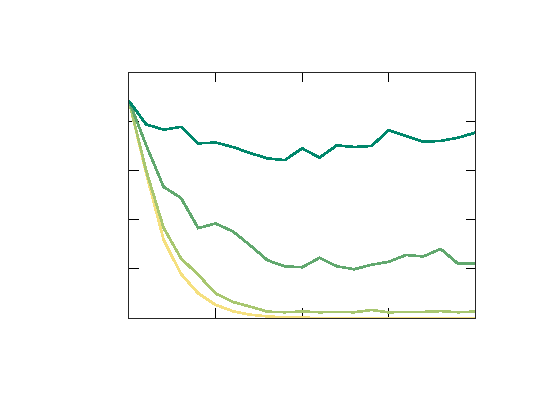
\includegraphics{./figures/parts/02/chapters/04/sections/03/tc_x1_non_convergence}}%
    \gplfronttext
  \end{picture}%
\endgroup

  \caption{\small Η εξέλιξη του μέτρου σφάλματος εκτίμησης θέσης για αυξανόμενες
           τιμές του μέτρου του σφάλματος εκτίμησης προσανατολισμού. Το τελικό
           σφάλμα θέσης είναι ανάλογο του αρχικού σφάλματος προσανατολισμού}
  \label{fig:02_04_03:tc_x1_non_convergence}
\end{figure}

\begin{gg_box}
\begin{remark}
  \label{remark:loc_prop_or}
  Χωρίς βλάβη της γενικότητας, μετά την εφαρμογή του Θεωρήματος
  \ref{prop:theorem_without_disturbance} το σφάλμα θέσης είναι ανάλογο με το
  σφάλμα προσανατολισμού.
\end{remark}
\end{gg_box}


%%%%%%%%%%%%%%%%%%%%%%%%%%%%%%%%%%%%%%%%%%%%%%%%%%%%%%%%%%%%%%%%%%%%%%%%%%%%%%%%
\section{Πειραματική αξιολόγηση}
  \label{section:02_03_04}
  Στο σχήμα \ref{fig:02_05_04:02} απεικονίζεται η διαδικασία ευθυγράμμισης δύο
πανοραμικών δισδιάστατων σαρώσεων που συνελήθησαν σε ένα περιβάλλον του συνόλου
δεδομένων \texttt{laserazos}\footref{foot:laserazos} μέσω των μεθόδων FastGICP
και FSM.  Εδώ παρατηρούμε πως ο πρώτος---όπως και όλες οι εκδόσεις του
ICP---εκτιμούν σταδιακά τον προσανατολισμό ανάμεσα στις δύο στάσεις από τις
οποίες συνελήφθησαν οι δύο σαρώσεις, σε αντίθεση με τον FSM, ο οποίος το κάνει
σε ένα βήμα---από εκεί και πέρα παρέχει όλο και πιο ακριβείς εκτιμήσεις μέσω
της υπερδειγματοληψίας του χάρτη $\widetilde{\bm{M}}$. Ο FastGICP χρησιμοποιεί
αντιστοιχίσεις για τα δύο σκέλη της ευθυγράμμισης, και ως εσωτερική μετρική το
μέτρο της εξ. (\ref{eq:sm_def}), ενώ ο FSM δεν χρησιμοποιεί αντιστοιχίσεις
όλως διόλου, και η εσωτερική μετρική του είναι η μετρική CAER (εξ.
(\ref{eq:caer_normal}), όπου $\mathcal{S}_R \leftarrow \mathcal{S}_1$,
$\mathcal{S}_V \leftarrow \mathcal{S}_0$, $(x,y,\theta)\leftarrow\bm{p}_1$, και
$(\hat{x}, \hat{y}, \hat{\theta}) \leftarrow \bm{p}_0$). Από τα αποτελέσματα
παρατηρούμε πως το σφάλμα εκτίμησης θέσης του FastGICP δεν ακολουθεί την
(μειούμενη) τροχιά της εσωτερικής του μετρικής---σε αντίθεση με αυτό του
FSM---και πως αυξάνει προτού στη συνέχεια μειωθεί, με αποτέλεσμα την
παγίδευση της εκτίμησης θέσης σε τοπικό ελάχιστο. Δεδομένου ότι οι συχνότητα
ανανέωσης μετρήσεων από τους εμπορικά διαθέσιμους πανοραμικούς αισθητήρες lidar
κυμαίνεται από $10$-$20$ Hz, με βάση την απόσταση των στάσεων από τις οποίες
συνελήφθησαν οι δύο μετρήσεις, συμπεραίνουμε πως ο FSM είναι ικανός εκτίμησης
της τροχιάς ενός ρομπότ το οποίο κινείται με ακτινική ταχύτητα $7.28$ m/s
($\approx 25$ km/h), και γωνιακή ταχύτητα $6\pi$ rad/s.

\begin{figure}[]\centering
  \definecolor{pp}{RGB}{127,201,127}
\definecolor{cc}{RGB}{0,0,0}
\definecolor{oo}{RGB}{251,128,114}

% GNUPLOT: LaTeX picture with Postscript
\begingroup
  \makeatletter
  \providecommand\color[2][]{%
    \GenericError{(gnuplot) \space\space\space\@spaces}{%
      Package color not loaded in conjunction with
      terminal option `colourtext'%
    }{See the gnuplot documentation for explanation.%
    }{Either use 'blacktext' in gnuplot or load the package
      color.sty in LaTeX.}%
    \renewcommand\color[2][]{}%
  }%
  \providecommand\includegraphics[2][]{%
    \GenericError{(gnuplot) \space\space\space\@spaces}{%
      Package graphicx or graphics not loaded%
    }{See the gnuplot documentation for explanation.%
    }{The gnuplot epslatex terminal needs graphicx.sty or graphics.sty.}%
    \renewcommand\includegraphics[2][]{}%
  }%
  \providecommand\rotatebox[2]{#2}%
  \@ifundefined{ifGPcolor}{%
    \newif\ifGPcolor
    \GPcolorfalse
  }{}%
  \@ifundefined{ifGPblacktext}{%
    \newif\ifGPblacktext
    \GPblacktexttrue
  }{}%
  % define a \g@addto@macro without @ in the name:
  \let\gplgaddtomacro\g@addto@macro
  % define empty templates for all commands taking text:
  \gdef\gplfronttext{}%
  \gdef\gplfronttext{}%
  \makeatother
  \ifGPblacktext
    % no textcolor at all
    \def\colorrgb#1{}%
    \def\colorgray#1{}%
  \else
    % gray or color?
    \ifGPcolor
      \def\colorrgb#1{\color[rgb]{#1}}%
      \def\colorgray#1{\color[gray]{#1}}%
      \expandafter\def\csname LTw\endcsname{\color{white}}%
      \expandafter\def\csname LTb\endcsname{\color{black}}%
      \expandafter\def\csname LTa\endcsname{\color{black}}%
      \expandafter\def\csname LT0\endcsname{\color[rgb]{1,0,0}}%
      \expandafter\def\csname LT1\endcsname{\color[rgb]{0,1,0}}%
      \expandafter\def\csname LT2\endcsname{\color[rgb]{0,0,1}}%
      \expandafter\def\csname LT3\endcsname{\color[rgb]{1,0,1}}%
      \expandafter\def\csname LT4\endcsname{\color[rgb]{0,1,1}}%
      \expandafter\def\csname LT5\endcsname{\color[rgb]{1,1,0}}%
      \expandafter\def\csname LT6\endcsname{\color[rgb]{0,0,0}}%
      \expandafter\def\csname LT7\endcsname{\color[rgb]{1,0.3,0}}%
      \expandafter\def\csname LT8\endcsname{\color[rgb]{0.5,0.5,0.5}}%
    \else
      % gray
      \def\colorrgb#1{\color{black}}%
      \def\colorgray#1{\color[gray]{#1}}%
      \expandafter\def\csname LTw\endcsname{\color{white}}%
      \expandafter\def\csname LTb\endcsname{\color{black}}%
      \expandafter\def\csname LTa\endcsname{\color{black}}%
      \expandafter\def\csname LT0\endcsname{\color{black}}%
      \expandafter\def\csname LT1\endcsname{\color{black}}%
      \expandafter\def\csname LT2\endcsname{\color{black}}%
      \expandafter\def\csname LT3\endcsname{\color{black}}%
      \expandafter\def\csname LT4\endcsname{\color{black}}%
      \expandafter\def\csname LT5\endcsname{\color{black}}%
      \expandafter\def\csname LT6\endcsname{\color{black}}%
      \expandafter\def\csname LT7\endcsname{\color{black}}%
      \expandafter\def\csname LT8\endcsname{\color{black}}%
    \fi
  \fi
    \setlength{\unitlength}{0.0500bp}%
    \ifx\gptboxheight\undefined%
      \newlength{\gptboxheight}%
      \newlength{\gptboxwidth}%
      \newsavebox{\gptboxtext}%
    \fi%
    \setlength{\fboxrule}{0.5pt}%
    \setlength{\fboxsep}{1pt}%
\begin{picture}(8000.00,8000.00)%
    \gplgaddtomacro\gplfronttext{%
    }%
    \gplgaddtomacro\gplfronttext{%
      \colorrgb{0.00,0.00,0.00}%
      \put(3999,7959){\makebox(0,0){\strut{}\small Αρχική συνθήκη}}%
      \put(600, 3770){\makebox(0,0){\strut{}{\color{pp}{\rule[0.6mm]{0.5cm}{0.5mm}}} \small Σφάλμα θέσης [m]}}
      \put(3420,3770){\makebox(0,0){\strut{}{\color{oo}{\rule[0.6mm]{0.5cm}{0.5mm}}} \small Σφάλμα προσανατολισμού [rad]}}
      \put(7020,3770){\makebox(0,0){\strut{}{\color{cc}{\rule[0.6mm]{0.5cm}{0.5mm}}} \small Οικεία εσωτερική μετρική σφάλματος [m]}}
    }%
    \gplgaddtomacro\gplfronttext{%
    }%
    \gplgaddtomacro\gplfronttext{%
      \colorrgb{0.00,0.00,0.00}%
      \put(1839,5959){\makebox(0,0){\strut{}\small Εξέλιξη ευθυγράμμισης FastGICP}}%
    }%
    \gplgaddtomacro\gplfronttext{%
    }%
    \gplgaddtomacro\gplfronttext{%
      \colorrgb{0.00,0.00,0.00}%
      \put(6159,5959){\makebox(0,0){\strut{}\small Εξέλιξη ευθυγράμμισης \texttt{fsm}}}%
    }%
    \gplgaddtomacro\gplfronttext{%
      \colorrgb{0.00,0.45,0.74}%
      \put(508,2400){\makebox(0,0)[r]{\strut{}\scriptsize $0.0$}}%
      \colorrgb{0.00,0.45,0.74}%
      \put(508,2543){\makebox(0,0)[r]{\strut{}\scriptsize $0.2$}}%
      \colorrgb{0.00,0.45,0.74}%
      \put(508,2685){\makebox(0,0)[r]{\strut{}\scriptsize $0.4$}}%
      \colorrgb{0.00,0.45,0.74}%
      \put(508,2828){\makebox(0,0)[r]{\strut{}\scriptsize $0.6$}}%
      \colorrgb{0.00,0.45,0.74}%
      \put(508,2971){\makebox(0,0)[r]{\strut{}\scriptsize $0.8$}}%
      \colorrgb{0.00,0.45,0.74}%
      \put(508,3114){\makebox(0,0)[r]{\strut{}\scriptsize $1.0$}}%
      \colorrgb{0.00,0.45,0.74}%
      \put(508,3256){\makebox(0,0)[r]{\strut{}\scriptsize $1.2$}}%
      \colorrgb{0.00,0.45,0.74}%
      \put(508,3399){\makebox(0,0)[r]{\strut{}\scriptsize $1.4$}}%
    }%
    \gplgaddtomacro\gplfronttext{%
    }%
    \gplgaddtomacro\gplfronttext{%
      \colorrgb{0.15,0.15,0.15}%
      \put(640,2180){\makebox(0,0){\strut{}\scriptsize $0$}}%
      \colorrgb{0.15,0.15,0.15}%
      \put(1089,2180){\makebox(0,0){\strut{}\scriptsize $10$}}%
      \colorrgb{0.15,0.15,0.15}%
      \put(1538,2180){\makebox(0,0){\strut{}\scriptsize $20$}}%
      \colorrgb{0.85,0.33,0.10}%
      \put(1715,2400){\makebox(0,0)[l]{\strut{}}}%
      \colorrgb{0.85,0.33,0.10}%
      \put(1715,2600){\makebox(0,0)[l]{\strut{}}}%
      \colorrgb{0.85,0.33,0.10}%
      \put(1715,2800){\makebox(0,0)[l]{\strut{}}}%
      \colorrgb{0.85,0.33,0.10}%
      \put(1715,2999){\makebox(0,0)[l]{\strut{}}}%
      \colorrgb{0.85,0.33,0.10}%
      \put(1715,3199){\makebox(0,0)[l]{\strut{}}}%
      \colorrgb{0.85,0.33,0.10}%
      \put(1715,3399){\makebox(0,0)[l]{\strut{}}}%
    }%
    \gplgaddtomacro\gplfronttext{%
    }%
    \gplgaddtomacro\gplfronttext{%
      \colorrgb{1.00,0.00,1.00}%
      \put(2108,2400){\makebox(0,0)[r]{\strut{}\scriptsize $0$}}%
      \colorrgb{1.00,0.00,1.00}%
      \put(2108,2574){\makebox(0,0)[r]{\strut{}\scriptsize $0.18$}}%
      \colorrgb{1.00,0.00,1.00}%
      \put(2108,2749){\makebox(0,0)[r]{\strut{}\scriptsize $0.35$}}%
      \colorrgb{1.00,0.00,1.00}%
      \put(2108,2923){\makebox(0,0)[r]{\strut{}\scriptsize $0.52$}}%
      \colorrgb{1.00,0.00,1.00}%
      \put(2108,3097){\makebox(0,0)[r]{\strut{}\scriptsize $0.70$}}%
      \colorrgb{1.00,0.00,1.00}%
      \put(2108,3272){\makebox(0,0)[r]{\strut{}\scriptsize $0.87$}}%
    }%
    \gplgaddtomacro\gplfronttext{%
    }%
    \gplgaddtomacro\gplfronttext{%
      \colorrgb{0.15,0.15,0.15}%
      \put(2240,2180){\makebox(0,0){\strut{}\scriptsize $0$}}%
      \colorrgb{0.15,0.15,0.15}%
      \put(2689,2180){\makebox(0,0){\strut{}\scriptsize $10$}}%
      \colorrgb{0.15,0.15,0.15}%
      \put(3138,2180){\makebox(0,0){\strut{}\scriptsize $20$}}%
      \colorrgb{0.85,0.33,0.10}%
      \put(3315,2400){\makebox(0,0)[l]{\strut{}\scriptsize $0$}}%
      \colorrgb{0.85,0.33,0.10}%
      \put(3315,2600){\makebox(0,0)[l]{\strut{}\scriptsize $100$}}%
      \colorrgb{0.85,0.33,0.10}%
      \put(3315,2800){\makebox(0,0)[l]{\strut{}\scriptsize $200$}}%
      \colorrgb{0.85,0.33,0.10}%
      \put(3315,2999){\makebox(0,0)[l]{\strut{}\scriptsize $300$}}%
      \colorrgb{0.85,0.33,0.10}%
      \put(3315,3199){\makebox(0,0)[l]{\strut{}\scriptsize $400$}}%
      \colorrgb{0.85,0.33,0.10}%
      \put(3315,3399){\makebox(0,0)[l]{\strut{}\scriptsize $500$}}%
    }%
    \gplgaddtomacro\gplfronttext{%
    }%
    \gplgaddtomacro\gplfronttext{%
      \colorrgb{0.00,0.45,0.74}%
      \put(4668,2400){\makebox(0,0)[r]{\strut{}\scriptsize $0.0$}}%
      \colorrgb{0.00,0.45,0.74}%
      \put(4668,2650){\makebox(0,0)[r]{\strut{}\scriptsize $0.1$}}%
      \colorrgb{0.00,0.45,0.74}%
      \put(4668,2900){\makebox(0,0)[r]{\strut{}\scriptsize $0.2$}}%
      \colorrgb{0.00,0.45,0.74}%
      \put(4668,3149){\makebox(0,0)[r]{\strut{}\scriptsize $0.3$}}%
      \colorrgb{0.00,0.45,0.74}%
      \put(4668,3399){\makebox(0,0)[r]{\strut{}\scriptsize $0.4$}}%
    }%
    \gplgaddtomacro\gplfronttext{%
    }%
    \gplgaddtomacro\gplfronttext{%
      \colorrgb{0.15,0.15,0.15}%
      \put(5010,2180){\makebox(0,0){\strut{}\scriptsize $2$}}%
      \colorrgb{0.15,0.15,0.15}%
      \put(5219,2180){\makebox(0,0){\strut{}\scriptsize $4$}}%
      \colorrgb{0.15,0.15,0.15}%
      \put(5429,2180){\makebox(0,0){\strut{}\scriptsize $6$}}%
      \colorrgb{0.15,0.15,0.15}%
      \put(5638,2180){\makebox(0,0){\strut{}\scriptsize $8$}}%
      \colorrgb{0.85,0.33,0.10}%
      \put(5875,2400){\makebox(0,0)[l]{\strut{}}}%
      \colorrgb{0.85,0.33,0.10}%
      \put(5875,2650){\makebox(0,0)[l]{\strut{}}}%
      \colorrgb{0.85,0.33,0.10}%
      \put(5875,2900){\makebox(0,0)[l]{\strut{}}}%
      \colorrgb{0.85,0.33,0.10}%
      \put(5875,3149){\makebox(0,0)[l]{\strut{}}}%
      \colorrgb{0.85,0.33,0.10}%
      \put(5875,3399){\makebox(0,0)[l]{\strut{}}}%
    }%
    \gplgaddtomacro\gplfronttext{%
    }%
    \gplgaddtomacro\gplfronttext{%
      \colorrgb{1.00,0.00,1.00}%
      \colorrgb{1.00,0.00,1.00}%
      \put(6268,2400){\makebox(0,0)[r]{\strut{}\scriptsize $0$}}%
      \colorrgb{1.00,0.00,1.00}%
      \put(6268,2574){\makebox(0,0)[r]{\strut{}\scriptsize $0.18$}}%
      \colorrgb{1.00,0.00,1.00}%
      \put(6268,2749){\makebox(0,0)[r]{\strut{}\scriptsize $0.35$}}%
      \colorrgb{1.00,0.00,1.00}%
      \put(6268,2923){\makebox(0,0)[r]{\strut{}\scriptsize $0.52$}}%
      \colorrgb{1.00,0.00,1.00}%
      \put(6268,3097){\makebox(0,0)[r]{\strut{}\scriptsize $0.70$}}%
      \colorrgb{1.00,0.00,1.00}%
      \put(6268,3272){\makebox(0,0)[r]{\strut{}\scriptsize $0.87$}}%
    }%
    \gplgaddtomacro\gplfronttext{%
    }%
    \gplgaddtomacro\gplfronttext{%
      \colorrgb{0.15,0.15,0.15}%
      \put(6610,2180){\makebox(0,0){\strut{}\scriptsize $2$}}%
      \colorrgb{0.15,0.15,0.15}%
      \put(6819,2180){\makebox(0,0){\strut{}\scriptsize $4$}}%
      \colorrgb{0.15,0.15,0.15}%
      \put(7029,2180){\makebox(0,0){\strut{}\scriptsize $6$}}%
      \colorrgb{0.15,0.15,0.15}%
      \put(7238,2180){\makebox(0,0){\strut{}\scriptsize $8$}}%
      \colorrgb{0.85,0.33,0.10}%
      \put(7475,2400){\makebox(0,0)[l]{\strut{}\scriptsize $0$}}%
      \colorrgb{0.85,0.33,0.10}%
      \put(7475,2650){\makebox(0,0)[l]{\strut{}\scriptsize $50$}}%
      \colorrgb{0.85,0.33,0.10}%
      \put(7475,2900){\makebox(0,0)[l]{\strut{}\scriptsize $100$}}%
      \colorrgb{0.85,0.33,0.10}%
      \put(7475,3149){\makebox(0,0)[l]{\strut{}\scriptsize $150$}}%
      \colorrgb{0.85,0.33,0.10}%
      \put(7475,3399){\makebox(0,0)[l]{\strut{}\scriptsize $200$}}%
    }%
    \gplgaddtomacro\gplfronttext{%
    }%
    \gplgaddtomacro\gplfronttext{%
    }%
    \gplgaddtomacro\gplfronttext{%
      \colorrgb{0.00,0.00,0.00}%
      \put(1839,1799){\makebox(0,0){\strut{}\small Τελική ευθυγράμμιση FastGICP}}%
    }%
    \gplgaddtomacro\gplfronttext{%
    }%
    \gplgaddtomacro\gplfronttext{%
      \colorrgb{0.00,0.00,0.00}%
      \put(6159,1799){\makebox(0,0){\strut{}\small Τελική ευθυγράμμιση \texttt{fsm}}}%
    }%
    \put(0,0){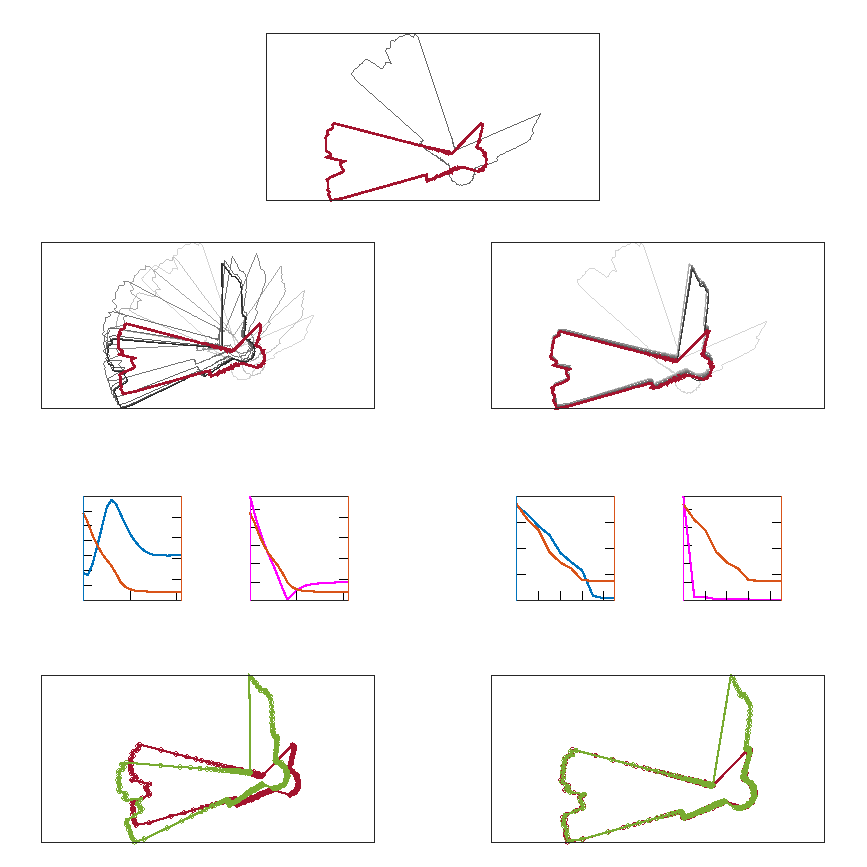
\includegraphics{./figures/parts/02/chapters/05/sections/04/fsm_vs_fgi}}%
    \gplfronttext
  \end{picture}%
\endgroup

  \vspace{0.5cm}
  \caption{\small Η εξέλιξη της διαδικασίας ευθυγράμμισης των δύο σαρώσεων του
           σχήματος της άνω σειράς μέσω του FastGICP (αριστερά) και του
           FSM (δεξιά). Οι δύο σαρώσεις διαταράσσονται από θόρυβο
           $\mathcal{N} \sim (0, 0.03^2)$ [m, m$^2$] και συλλαμβάνονται από
           στάσεις με διαφορά $\Delta = (0.35, 0.10, -\pi/3)$ [m,m,rad].
           Τα τελικά σφάλματα θέσης και προσανατολισμού του FastGICP είναι
           $0.61$ m και $0.173$ rad αντίστοιχα, ενώ του FSM
           $0.0098$ m και $0.0014$ rad}
  \label{fig:02_05_04:02}
\end{figure}


Στο σχήμα \ref{fig:02_05_04:01} απεικονίζεται η χρησιμότητα της ευθυγράμμισης
σαρώσεων: σε συνθήκες απουσίας χάρτη του περιβάλλοντος μία μέθοδος
ευθυγράμμισης σαρώσεων δρα ως παρατηρητής της στάσης ενός ρομπότ. Στο πρόβλημα
της ευθυγράμμισης πραγματικών με εικονικές σαρώσεις (κεφ.
\ref{part:02:chapter:04}) ο χάρτης δρα ως μέσο ανάδρασης λόγω της αντιστοιχίας
του με το περιβάλλον και του σταθερού συστήματος αναφοράς που ο ίδιος
παρέχει---η απουσία του εδώ, συνεπώς, αφαιρεί και τη δυνατότητα φραγής του
σφάλματος εκτίμησης.\footnote{Η ίδια απουσία σταθερού συστήματος αναφοράς
βαραίνει και την εκτίμηση της στάσης του ρομπότ μέσω κωδικοποιητών.} Στο σχήμα
\ref{fig:02_05_04:01} παρατηρούμε πως σε ιδανικές συνθήκες ($\sigma_R = 0.0$ m)
οι PLICP και NDT εισάγουν οι ίδιες σφάλματα εκτίμησης---πιθανότατα λόγω
αποστάσεων θέσης και προσανατολισμού με μέτρο μεγαλύτερο από ότι μπορούν να
διορθώσουν με μεγαλύτερη ακρίβεια. Σε συνθήκες όπου ο αισθητήρας λαμβάνει
αραιότερα δείγματα στο χώρο αυτές οι αποστάσεις αυξάνουν, με αποτέλεσμα
αυξημένα σφάλματα. Σε αντίθεση ο FSM είναι ικανός να παρατηρήσει την τροχιά του
αισθητήρα με μεγαλύτερη ακρίβεια.

\begin{figure}[]\centering
  \begin{subfigure}{\linewidth}
    % GNUPLOT: LaTeX picture with Postscript
\begingroup
  \makeatletter
  \providecommand\color[2][]{%
    \GenericError{(gnuplot) \space\space\space\@spaces}{%
      Package color not loaded in conjunction with
      terminal option `colourtext'%
    }{See the gnuplot documentation for explanation.%
    }{Either use 'blacktext' in gnuplot or load the package
      color.sty in LaTeX.}%
    \renewcommand\color[2][]{}%
  }%
  \providecommand\includegraphics[2][]{%
    \GenericError{(gnuplot) \space\space\space\@spaces}{%
      Package graphicx or graphics not loaded%
    }{See the gnuplot documentation for explanation.%
    }{The gnuplot epslatex terminal needs graphicx.sty or graphics.sty.}%
    \renewcommand\includegraphics[2][]{}%
  }%
  \providecommand\rotatebox[2]{#2}%
  \@ifundefined{ifGPcolor}{%
    \newif\ifGPcolor
    \GPcolorfalse
  }{}%
  \@ifundefined{ifGPblacktext}{%
    \newif\ifGPblacktext
    \GPblacktexttrue
  }{}%
  % define a \g@addto@macro without @ in the name:
  \let\gplgaddtomacro\g@addto@macro
  % define empty templates for all commands taking text:
  \gdef\gplbacktext{}%
  \gdef\gplfronttext{}%
  \makeatother
  \ifGPblacktext
    % no textcolor at all
    \def\colorrgb#1{}%
    \def\colorgray#1{}%
  \else
    % gray or color?
    \ifGPcolor
      \def\colorrgb#1{\color[rgb]{#1}}%
      \def\colorgray#1{\color[gray]{#1}}%
      \expandafter\def\csname LTw\endcsname{\color{white}}%
      \expandafter\def\csname LTb\endcsname{\color{black}}%
      \expandafter\def\csname LTa\endcsname{\color{black}}%
      \expandafter\def\csname LT0\endcsname{\color[rgb]{1,0,0}}%
      \expandafter\def\csname LT1\endcsname{\color[rgb]{0,1,0}}%
      \expandafter\def\csname LT2\endcsname{\color[rgb]{0,0,1}}%
      \expandafter\def\csname LT3\endcsname{\color[rgb]{1,0,1}}%
      \expandafter\def\csname LT4\endcsname{\color[rgb]{0,1,1}}%
      \expandafter\def\csname LT5\endcsname{\color[rgb]{1,1,0}}%
      \expandafter\def\csname LT6\endcsname{\color[rgb]{0,0,0}}%
      \expandafter\def\csname LT7\endcsname{\color[rgb]{1,0.3,0}}%
      \expandafter\def\csname LT8\endcsname{\color[rgb]{0.5,0.5,0.5}}%
    \else
      % gray
      \def\colorrgb#1{\color{black}}%
      \def\colorgray#1{\color[gray]{#1}}%
      \expandafter\def\csname LTw\endcsname{\color{white}}%
      \expandafter\def\csname LTb\endcsname{\color{black}}%
      \expandafter\def\csname LTa\endcsname{\color{black}}%
      \expandafter\def\csname LT0\endcsname{\color{black}}%
      \expandafter\def\csname LT1\endcsname{\color{black}}%
      \expandafter\def\csname LT2\endcsname{\color{black}}%
      \expandafter\def\csname LT3\endcsname{\color{black}}%
      \expandafter\def\csname LT4\endcsname{\color{black}}%
      \expandafter\def\csname LT5\endcsname{\color{black}}%
      \expandafter\def\csname LT6\endcsname{\color{black}}%
      \expandafter\def\csname LT7\endcsname{\color{black}}%
      \expandafter\def\csname LT8\endcsname{\color{black}}%
    \fi
  \fi
    \setlength{\unitlength}{0.0500bp}%
    \ifx\gptboxheight\undefined%
      \newlength{\gptboxheight}%
      \newlength{\gptboxwidth}%
      \newsavebox{\gptboxtext}%
    \fi%
    \setlength{\fboxrule}{0.5pt}%
    \setlength{\fboxsep}{1pt}%
\begin{picture}(7000.00,7000.00)%
    \gplgaddtomacro\gplbacktext{%
      \colorrgb{0.15,0.15,0.15}%
      \put(600,2189){\makebox(0,0)[r]{\strut{}6}}%
      \colorrgb{0.15,0.15,0.15}%
      \put(600,2784){\makebox(0,0)[r]{\strut{}8}}%
      \colorrgb{0.15,0.15,0.15}%
      \put(600,3378){\makebox(0,0)[r]{\strut{}10}}%
      \colorrgb{0.15,0.15,0.15}%
      \put(600,3973){\makebox(0,0)[r]{\strut{}12}}%
      \colorrgb{0.15,0.15,0.15}%
      \put(600,4567){\makebox(0,0)[r]{\strut{}14}}%
      \colorrgb{0.15,0.15,0.15}%
      \put(600,5162){\makebox(0,0)[r]{\strut{}16}}%
      \colorrgb{0.00,0.00,0.00}%
      \put(940,1880){\makebox(0,0){\strut{}-2}}%
      \colorrgb{0.00,0.00,0.00}%
      \put(1535,1880){\makebox(0,0){\strut{}0}}%
      \colorrgb{0.00,0.00,0.00}%
      \put(2129,1880){\makebox(0,0){\strut{}2}}%
      \colorrgb{0.00,0.00,0.00}%
      \put(2724,1880){\makebox(0,0){\strut{}4}}%
      \colorrgb{0.00,0.00,0.00}%
      \put(3318,1880){\makebox(0,0){\strut{}6}}%
    }%
    \gplgaddtomacro\gplfronttext{%
    }%
    \gplgaddtomacro\gplbacktext{%
      \colorrgb{0.00,0.00,0.00}%
      \put(3950,1880){\makebox(0,0){\strut{}-2}}%
      \colorrgb{0.00,0.00,0.00}%
      \put(4544,1880){\makebox(0,0){\strut{}0}}%
      \colorrgb{0.00,0.00,0.00}%
      \put(5139,1880){\makebox(0,0){\strut{}2}}%
      \colorrgb{0.00,0.00,0.00}%
      \put(5733,1880){\makebox(0,0){\strut{}4}}%
      \colorrgb{0.00,0.00,0.00}%
      \put(6327,1880){\makebox(0,0){\strut{}6}}%
    }%
    \gplgaddtomacro\gplfronttext{%
    }%
    \gplbacktext
    \put(0,0){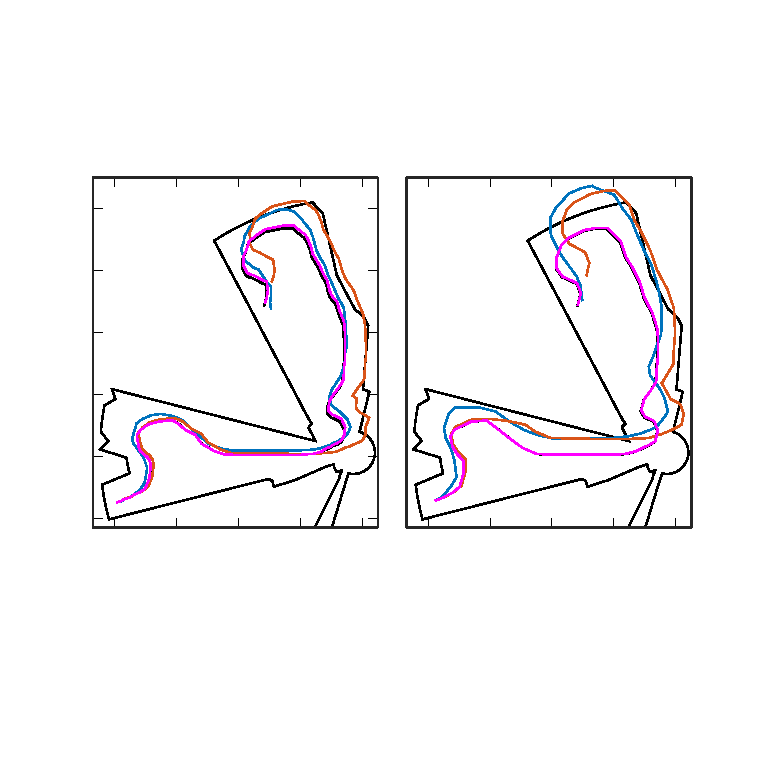
\includegraphics{/media/li9i/var/elements/PhD/fourier_scan_matcher/scripts_phd/characterisation/laser_odometry/odom_test_5_vs_6_sr_000}}%
    \gplfronttext
  \end{picture}%
\endgroup

  \end{subfigure}\\ \vspace{-5cm}
  \begin{subfigure}{\linewidth}
    % GNUPLOT: LaTeX picture with Postscript
\begingroup
  \makeatletter
  \providecommand\color[2][]{%
    \GenericError{(gnuplot) \space\space\space\@spaces}{%
      Package color not loaded in conjunction with
      terminal option `colourtext'%
    }{See the gnuplot documentation for explanation.%
    }{Either use 'blacktext' in gnuplot or load the package
      color.sty in LaTeX.}%
    \renewcommand\color[2][]{}%
  }%
  \providecommand\includegraphics[2][]{%
    \GenericError{(gnuplot) \space\space\space\@spaces}{%
      Package graphicx or graphics not loaded%
    }{See the gnuplot documentation for explanation.%
    }{The gnuplot epslatex terminal needs graphicx.sty or graphics.sty.}%
    \renewcommand\includegraphics[2][]{}%
  }%
  \providecommand\rotatebox[2]{#2}%
  \@ifundefined{ifGPcolor}{%
    \newif\ifGPcolor
    \GPcolorfalse
  }{}%
  \@ifundefined{ifGPblacktext}{%
    \newif\ifGPblacktext
    \GPblacktexttrue
  }{}%
  % define a \g@addto@macro without @ in the name:
  \let\gplgaddtomacro\g@addto@macro
  % define empty templates for all commands taking text:
  \gdef\gplfronttext{}%
  \gdef\gplfronttext{}%
  \makeatother
  \ifGPblacktext
    % no textcolor at all
    \def\colorrgb#1{}%
    \def\colorgray#1{}%
  \else
    % gray or color?
    \ifGPcolor
      \def\colorrgb#1{\color[rgb]{#1}}%
      \def\colorgray#1{\color[gray]{#1}}%
      \expandafter\def\csname LTw\endcsname{\color{white}}%
      \expandafter\def\csname LTb\endcsname{\color{black}}%
      \expandafter\def\csname LTa\endcsname{\color{black}}%
      \expandafter\def\csname LT0\endcsname{\color[rgb]{1,0,0}}%
      \expandafter\def\csname LT1\endcsname{\color[rgb]{0,1,0}}%
      \expandafter\def\csname LT2\endcsname{\color[rgb]{0,0,1}}%
      \expandafter\def\csname LT3\endcsname{\color[rgb]{1,0,1}}%
      \expandafter\def\csname LT4\endcsname{\color[rgb]{0,1,1}}%
      \expandafter\def\csname LT5\endcsname{\color[rgb]{1,1,0}}%
      \expandafter\def\csname LT6\endcsname{\color[rgb]{0,0,0}}%
      \expandafter\def\csname LT7\endcsname{\color[rgb]{1,0.3,0}}%
      \expandafter\def\csname LT8\endcsname{\color[rgb]{0.5,0.5,0.5}}%
    \else
      % gray
      \def\colorrgb#1{\color{black}}%
      \def\colorgray#1{\color[gray]{#1}}%
      \expandafter\def\csname LTw\endcsname{\color{white}}%
      \expandafter\def\csname LTb\endcsname{\color{black}}%
      \expandafter\def\csname LTa\endcsname{\color{black}}%
      \expandafter\def\csname LT0\endcsname{\color{black}}%
      \expandafter\def\csname LT1\endcsname{\color{black}}%
      \expandafter\def\csname LT2\endcsname{\color{black}}%
      \expandafter\def\csname LT3\endcsname{\color{black}}%
      \expandafter\def\csname LT4\endcsname{\color{black}}%
      \expandafter\def\csname LT5\endcsname{\color{black}}%
      \expandafter\def\csname LT6\endcsname{\color{black}}%
      \expandafter\def\csname LT7\endcsname{\color{black}}%
      \expandafter\def\csname LT8\endcsname{\color{black}}%
    \fi
  \fi
    \setlength{\unitlength}{0.02500bp}%
    \ifx\gptboxheight\undefined%
      \newlength{\gptboxheight}%
      \newlength{\gptboxwidth}%
      \newsavebox{\gptboxtext}%
    \fi%
    \setlength{\fboxrule}{0.5pt}%
    \setlength{\fboxsep}{1pt}%
\hspace{1cm}
\begin{picture}(7000.00,7000.00)%
    \gplgaddtomacro\gplfronttext{%
      \colorrgb{0.15,0.15,0.15}%
      \put(600,2189){\makebox(0,0)[r]{\strut{}\scriptsize $6.0$}}%
      \colorrgb{0.15,0.15,0.15}%
      \put(600,2784){\makebox(0,0)[r]{\strut{}\scriptsize $8.0$}}%
      \colorrgb{0.15,0.15,0.15}%
      \put(600,3378){\makebox(0,0)[r]{\strut{}\scriptsize $10.0$}}%
      \colorrgb{0.15,0.15,0.15}%
      \put(600,3973){\makebox(0,0)[r]{\strut{}\scriptsize $12.0$}}%
      \colorrgb{0.15,0.15,0.15}%
      \put(600,4567){\makebox(0,0)[r]{\strut{}\scriptsize $14.0$}}%
      \colorrgb{0.15,0.15,0.15}%
      \put(600,5162){\makebox(0,0)[r]{\strut{}\scriptsize $16.0$}}%
      \colorrgb{0.00,0.00,0.00}%
      \put(940,1880){\makebox(0,0){\strut{} \scriptsize $-2.0$}}%
      \colorrgb{0.00,0.00,0.00}%
      %\put(1535,1880){\makebox(0,0){\strut{}\scriptsize $0.0$}}%
      \colorrgb{0.00,0.00,0.00}%
      \put(2129,1880){\makebox(0,0){\strut{}\scriptsize $2.0$}}%
      \colorrgb{0.00,0.00,0.00}%
      \put(2724,1880){\makebox(0,0){\strut{}\scriptsize $4.0$}}%
      \colorrgb{0.00,0.00,0.00}%
      \put(3318,1880){\makebox(0,0){\strut{}\scriptsize $6.0$}}%

      \put(-800,4900){\rotatebox{90}{\makebox(0,0)[r]{\strut{}$\sigma_R = 0.05$ m}}}%
      \put(1800,1504){\makebox(0,0){\strut{} \scriptsize Συχνές μετρήσεις}}
      \put(5100,1504){\makebox(0,0){\strut{} \scriptsize Σποραδικές μετρήσεις}}
    }%
    \gplgaddtomacro\gplfronttext{%
    }%
    \gplgaddtomacro\gplfronttext{%
      \colorrgb{0.00,0.00,0.00}%
      \put(3950,1880){\makebox(0,0){\strut{}\scriptsize $-2.0$}}%
      \colorrgb{0.00,0.00,0.00}%
      %\put(4544,1880){\makebox(0,0){\strut{}\scriptsize $0.0$}}%
      \colorrgb{0.00,0.00,0.00}%
      \put(5139,1880){\makebox(0,0){\strut{}\scriptsize $2.0$}}%
      \colorrgb{0.00,0.00,0.00}%
      \put(5733,1880){\makebox(0,0){\strut{}\scriptsize $4.0$}}%
      \colorrgb{0.00,0.00,0.00}%
      \put(6327,1880){\makebox(0,0){\strut{}\scriptsize $6.0$}}%
    }%
    \gplgaddtomacro\gplfronttext{%
    }%
    \put(0,0){\animategraphics[autoplay,scale=0.5]{10}{./figures/slides/ch7/odom/sim/laser_odometry/imgs/odom_test_5_vs_6_sr_005_}{1}{110}}%
    \gplfronttext
  \end{picture}%
\endgroup

  \end{subfigure}
  \vspace{-2cm}
  \caption{\small Η ευθυγράμμιση σαρώσεων ως μέσο παρατήρησης της τροχιάς του
           αισθητήρα, ή αλλιώς ως ``laser odometry": το ρομπότ κινείται από
           την κάτω αριστερά περιοχή του περιβάλλοντος προς την άνω δεξιά,
           συλλαμβάνοντας μετρήσεις καθ' οδόν. Οι χρωματισμένες γραμμές
           απεικονίζουν τις εκτιμώμενες τροχιές του αισθητήρα από κάθε μέθοδο.
           Στα διαγράμματα της αριστερής πλευράς ο αισθητήρας αποστάσεων
           συλλέγει συχνότερα μετρήσεις από ότι στα διαγράμματα της δεξιάς
           πλευράς, με αποτέλεσμα πυκνότερες μετρήσεις στο χώρο, συλληφθείσες
           από στάσεις με μικρότερη απόσταση θέσεων, και συνεπώς με
           μεγαλύτερη αλληλοεπικάλυψη. Στα διαγράμματα της άνω σειράς ο
           αισθητήρας αναφέρει τέλειες μετρήσεις, ενώ στα διαγράμματα της κάτω
           σειράς μετρήσεις στις οποίες επιδρούν διαταραχές
           $\mathcal{N}\sim(0,0.05^2)$ [m,m$^2$]}
  \label{fig:02_05_04:01}
\end{figure}


Οι κύριοι περιορισμοί της απόκρισης των μεθόδων ευθυγράμμισης σαρώσεων είναι οι
ίδιοι με αυτούς των προσθετικών μεθόδων ευθυγράμμισης πραγματικών με εικονικές
σαρώσεις. Αυτοί αφορούν στα αμετάβλητα χαρακτηριστικά μεγέθη του φυσικού
αισθητήρα σαρώσεων, τα οποία είναι δυο. Το πρώτο είναι το μέγεθος των
διαταραχών που επιδρούν στις μετρήσεις του, την απόκριση επί του οποίου
εξετάσαμε για διάφορες τιμές στην ενότητα \ref{section:02_05_03}. Το δεύτερο
είναι το βεληνεκές του αισθητήρα, δηλαδή η μέγιστη απόσταση μέχρι την οποία
μπορεί να ανιχνεύσει την παρουσία αντικειμένων.

Στην άνω σειρά του σχήματος \ref{fig:02_05_04:03} εμφανίζονται με λευκό χρώμα
δύο διαφορετικά περιβάλλοντα, μέσα στα οποία τοποθετείται ένας αισθητήρας στις
θέσεις που σημειώνονται με κουκκίδες βαθύ μπλε χρώματος. Οι θέσεις αυτές είναι
τα κέντρα των ομόκεντρων κύκλων που εμφανίζονται στην ίδια σειρά. Η πειραματική
διάταξη που ακολουθεί στοχεύει στην καταγραφή της απόκρισης των μεθόδων
PLICP και FSM σε πειράματα όπου το βεληνεκές του αισθητήρα
μεταβάλλεται έτσι ώστε οι μετρήσεις του να περιλαμβάνουν όλα τα εμπόδια του
περιβάλλοντος, μειούμενο μέχρι που να μην περιλαμβάνουν κανένα. Το βεληνεκές
του αισθητήρα είναι η ακτίνα των κύκλων της πρώτης σειράς του σχήματος, και το
χρώμα αυτών αναπαριστά το ποσοστό των ακτίνων που φέρουν χωρική πληροφορία,
βάσει της χρωματικής λωρίδας που παρουσιάζεται στη δεύτερη σειρά. Στις δύο
τελευταίες σειρές παρατίθενται οι μέσοι όροι των σφαλμάτων εκτίμησης
προσανατολισμού και θέσης σε δέκα επαναλήψεις, για κάθε μέθοδο και περιβάλλον,
για $\sigma_R = 0.05$ m. Η δεύτερη στάση του αισθητήρα παράγεται τυχαία για
κάθε πείραμα μέσω διαταραχής των αντίστοιχων συνιστωσών της πρώτης στάσης του
αισθητήρα με ποσότητες που εξάγονται από τις ομοιόμορφες κατανομές
$U_{xy}(-\overline{\delta}_{xy},+\overline{\delta}_{xy})$ m και
$U_{\theta}(-\overline{\delta}_{\theta},+\overline{\delta}_{\theta})$ rad.
Συγκεκριμένα δοκιμάζονται δύο διαμορφώσεις αρχικών συνθηκών. H πρώτη
συμβολίζεται με $\Delta_\alpha$, για την οποία
$(\overline{\delta}_{xy}, \overline{\delta}_{\theta}) = (0.05,0.174)$ [m,rad].
Η δεύτερη συμβολίζεται με $\Delta_\beta$, για την οποία
$(\overline{\delta}_{xy},\overline{\delta}_{\theta}) = (0.20,\pi/4)$ [m,rad].

\begin{figure}[]\centering
  \definecolor{aa}{rgb}{0.00000   0.44700   0.74100}
\definecolor{ac}{rgb}{1.00000   0.00000   1.00000}

% GNUPLOT: LaTeX picture with Postscript
\begingroup
  \makeatletter
  \providecommand\color[2][]{%
    \GenericError{(gnuplot) \space\space\space\@spaces}{%
      Package color not loaded in conjunction with
      terminal option `colourtext'%
    }{See the gnuplot documentation for explanation.%
    }{Either use 'blacktext' in gnuplot or load the package
      color.sty in LaTeX.}%
    \renewcommand\color[2][]{}%
  }%
  \providecommand\includegraphics[2][]{%
    \GenericError{(gnuplot) \space\space\space\@spaces}{%
      Package graphicx or graphics not loaded%
    }{See the gnuplot documentation for explanation.%
    }{The gnuplot epslatex terminal needs graphicx.sty or graphics.sty.}%
    \renewcommand\includegraphics[2][]{}%
  }%
  \providecommand\rotatebox[2]{#2}%
  \@ifundefined{ifGPcolor}{%
    \newif\ifGPcolor
    \GPcolorfalse
  }{}%
  \@ifundefined{ifGPblacktext}{%
    \newif\ifGPblacktext
    \GPblacktexttrue
  }{}%
  % define a \g@addto@macro without @ in the name:
  \let\gplgaddtomacro\g@addto@macro
  % define empty templates for all commands taking text:
  \gdef\gplfronttext{}%
  \gdef\gplfronttext{}%
  \makeatother
  \ifGPblacktext
    % no textcolor at all
    \def\colorrgb#1{}%
    \def\colorgray#1{}%
  \else
    % gray or color?
    \ifGPcolor
      \def\colorrgb#1{\color[rgb]{#1}}%
      \def\colorgray#1{\color[gray]{#1}}%
      \expandafter\def\csname LTw\endcsname{\color{white}}%
      \expandafter\def\csname LTb\endcsname{\color{black}}%
      \expandafter\def\csname LTa\endcsname{\color{black}}%
      \expandafter\def\csname LT0\endcsname{\color[rgb]{1,0,0}}%
      \expandafter\def\csname LT1\endcsname{\color[rgb]{0,1,0}}%
      \expandafter\def\csname LT2\endcsname{\color[rgb]{0,0,1}}%
      \expandafter\def\csname LT3\endcsname{\color[rgb]{1,0,1}}%
      \expandafter\def\csname LT4\endcsname{\color[rgb]{0,1,1}}%
      \expandafter\def\csname LT5\endcsname{\color[rgb]{1,1,0}}%
      \expandafter\def\csname LT6\endcsname{\color[rgb]{0,0,0}}%
      \expandafter\def\csname LT7\endcsname{\color[rgb]{1,0.3,0}}%
      \expandafter\def\csname LT8\endcsname{\color[rgb]{0.5,0.5,0.5}}%
    \else
      % gray
      \def\colorrgb#1{\color{black}}%
      \def\colorgray#1{\color[gray]{#1}}%
      \expandafter\def\csname LTw\endcsname{\color{white}}%
      \expandafter\def\csname LTb\endcsname{\color{black}}%
      \expandafter\def\csname LTa\endcsname{\color{black}}%
      \expandafter\def\csname LT0\endcsname{\color{black}}%
      \expandafter\def\csname LT1\endcsname{\color{black}}%
      \expandafter\def\csname LT2\endcsname{\color{black}}%
      \expandafter\def\csname LT3\endcsname{\color{black}}%
      \expandafter\def\csname LT4\endcsname{\color{black}}%
      \expandafter\def\csname LT5\endcsname{\color{black}}%
      \expandafter\def\csname LT6\endcsname{\color{black}}%
      \expandafter\def\csname LT7\endcsname{\color{black}}%
      \expandafter\def\csname LT8\endcsname{\color{black}}%
    \fi
  \fi
    \setlength{\unitlength}{0.0500bp}%
    \ifx\gptboxheight\undefined%
      \newlength{\gptboxheight}%
      \newlength{\gptboxwidth}%
      \newsavebox{\gptboxtext}%
    \fi%
    \setlength{\fboxrule}{0.5pt}%
    \setlength{\fboxsep}{1pt}%
\begin{picture}(8000.00,10000.00)%
    \gplgaddtomacro\gplfronttext{%
    }%
    \gplgaddtomacro\gplfronttext{%
    }%
    \gplgaddtomacro\gplfronttext{%
    }%
    \gplgaddtomacro\gplfronttext{%
    }%
    \gplgaddtomacro\gplfronttext{%
    }%
    \gplgaddtomacro\gplfronttext{%
      \colorrgb{0.00,0.00,0.00}%
      \put(3999,7219){\makebox(0,0){\strut{}Χρωματική αναπαράσταση ποσοστού ακτίνων εντός μέγιστου εύρους αισθητήρα}}%
    }%
    \gplgaddtomacro\gplfronttext{%
    }%
    \gplgaddtomacro\gplfronttext{%
      \colorrgb{0.15,0.15,0.15}%
      \put(1040,6580){\makebox(0,0){\strut{}\small $0\%$}}%
      \colorrgb{0.15,0.15,0.15}%
      \put(2280,6580){\makebox(0,0){\strut{}\small $20\%$}}%
      \colorrgb{0.15,0.15,0.15}%
      \put(3520,6580){\makebox(0,0){\strut{}\small $40\%$}}%
      \colorrgb{0.15,0.15,0.15}%
      \put(4759,6580){\makebox(0,0){\strut{}\small $60\%$}}%
      \colorrgb{0.15,0.15,0.15}%
      \put(5999,6580){\makebox(0,0){\strut{}\small $80\%$}}%
      \colorrgb{0.15,0.15,0.15}%
      \put(7239,6580){\makebox(0,0){\strut{}\small $100\%$}}%
    }%
    \gplgaddtomacro\gplfronttext{%
      \colorrgb{0.15,0.15,0.15}%
      \put(768,4000){\makebox(0,0)[r]{\strut{}\scriptsize $0.0$}}%
      \colorrgb{0.15,0.15,0.15}%
      \put(768,4374){\makebox(0,0)[r]{\strut{}\scriptsize $0.035$}}%
      \colorrgb{0.15,0.15,0.15}%
      \put(768,4747){\makebox(0,0)[r]{\strut{}\scriptsize $0.070$}}%
      \colorrgb{0.15,0.15,0.15}%
      \put(768,5121){\makebox(0,0)[r]{\strut{}\scriptsize $0.105$}}%
      \colorrgb{0.15,0.15,0.15}%
      \put(768,5495){\makebox(0,0)[r]{\strut{}\scriptsize $0.140$}}%
      \colorrgb{0.15,0.15,0.15}%
      \put(800,3780){\makebox(0,0){\strut{}}}%
      \colorrgb{0.15,0.15,0.15}%
      \put(1040,3780){\makebox(0,0){\strut{}}}%
      \colorrgb{0.15,0.15,0.15}%
      \put(1280,3780){\makebox(0,0){\strut{}}}%
      \colorrgb{0.15,0.15,0.15}%
      \put(1519,3780){\makebox(0,0){\strut{}}}%
      \colorrgb{0.15,0.15,0.15}%
      \put(1759,3780){\makebox(0,0){\strut{}}}%
      \colorrgb{0.15,0.15,0.15}%
      \put(1999,3780){\makebox(0,0){\strut{}}}%
    }%
    \gplgaddtomacro\gplfronttext{%
      \colorrgb{0.15,0.15,0.15}%
      \put(-200,4749){\rotatebox{90}{\makebox(0,0){\strut{}$e_{\theta}$ [rad]}}}%
      \colorrgb{0.00,0.00,0.00}%
      \put(1399,5719){\makebox(0,0){\strut{}$\Delta_{\alpha}$}}%
    }%
    \gplgaddtomacro\gplfronttext{%
      \colorrgb{0.15,0.15,0.15}%
      \put(2448,4000){\makebox(0,0)[r]{\strut{}\scriptsize $0.0$}}%
      \colorrgb{0.15,0.15,0.15}%
      \put(2448,4503){\makebox(0,0)[r]{\strut{}\scriptsize $0.17$}}%
      \colorrgb{0.15,0.15,0.15}%
      \put(2448,5006){\makebox(0,0)[r]{\strut{}\scriptsize $0.35$}}%
      \colorrgb{0.15,0.15,0.15}%
      \put(2480,3780){\makebox(0,0){\strut{}}}%
      \colorrgb{0.15,0.15,0.15}%
      \put(2720,3780){\makebox(0,0){\strut{}}}%
      \colorrgb{0.15,0.15,0.15}%
      \put(2960,3780){\makebox(0,0){\strut{}}}%
      \colorrgb{0.15,0.15,0.15}%
      \put(3199,3780){\makebox(0,0){\strut{}}}%
      \colorrgb{0.15,0.15,0.15}%
      \put(3439,3780){\makebox(0,0){\strut{}}}%
      \colorrgb{0.15,0.15,0.15}%
      \put(3679,3780){\makebox(0,0){\strut{}}}%
    }%
    \gplgaddtomacro\gplfronttext{%
      \colorrgb{0.00,0.00,0.00}%
      \put(3079,5719){\makebox(0,0){\strut{}$\Delta_{\beta}$}}%
    }%
    \gplgaddtomacro\gplfronttext{%
      \colorrgb{0.15,0.15,0.15}%
      \put(4688,4000){\makebox(0,0)[r]{\strut{}\scriptsize $0.0$}}%
      \colorrgb{0.15,0.15,0.15}%
      \put(4688,4374){\makebox(0,0)[r]{\strut{}\scriptsize $0.035$}}%
      \colorrgb{0.15,0.15,0.15}%
      \put(4688,4747){\makebox(0,0)[r]{\strut{}\scriptsize $0.070$}}%
      \colorrgb{0.15,0.15,0.15}%
      \put(4688,5121){\makebox(0,0)[r]{\strut{}\scriptsize $0.105$}}%
      \colorrgb{0.15,0.15,0.15}%
      \put(4688,5495){\makebox(0,0)[r]{\strut{}\scriptsize $0.140$}}%
      \colorrgb{0.15,0.15,0.15}%
      \put(4720,3780){\makebox(0,0){\strut{}}}%
      \colorrgb{0.15,0.15,0.15}%
      \put(4960,3780){\makebox(0,0){\strut{}}}%
      \colorrgb{0.15,0.15,0.15}%
      \put(5200,3780){\makebox(0,0){\strut{}}}%
      \colorrgb{0.15,0.15,0.15}%
      \put(5439,3780){\makebox(0,0){\strut{}}}%
      \colorrgb{0.15,0.15,0.15}%
      \put(5679,3780){\makebox(0,0){\strut{}}}%
      \colorrgb{0.15,0.15,0.15}%
      \put(5919,3780){\makebox(0,0){\strut{}}}%
    }%
    \gplgaddtomacro\gplfronttext{%
      \colorrgb{0.00,0.00,0.00}%
      \put(5319,5719){\makebox(0,0){\strut{}$\Delta_{\alpha}$}}%
    }%
    \gplgaddtomacro\gplfronttext{%
      \colorrgb{0.15,0.15,0.15}%
      \put(6368,4000){\makebox(0,0)[r]{\strut{}\scriptsize $0.0$}}%
      \colorrgb{0.15,0.15,0.15}%
      \put(6368,4503){\makebox(0,0)[r]{\strut{}\scriptsize $0.17$}}%
      \colorrgb{0.15,0.15,0.15}%
      \put(6368,5006){\makebox(0,0)[r]{\strut{}\scriptsize $0.35$}}%
      \colorrgb{0.15,0.15,0.15}%
      \put(6400,3780){\makebox(0,0){\strut{}}}%
      \colorrgb{0.15,0.15,0.15}%
      \put(6640,3780){\makebox(0,0){\strut{}}}%
      \colorrgb{0.15,0.15,0.15}%
      \put(6880,3780){\makebox(0,0){\strut{}}}%
      \colorrgb{0.15,0.15,0.15}%
      \put(7119,3780){\makebox(0,0){\strut{}}}%
      \colorrgb{0.15,0.15,0.15}%
      \put(7359,3780){\makebox(0,0){\strut{}}}%
      \colorrgb{0.15,0.15,0.15}%
      \put(7599,3780){\makebox(0,0){\strut{}}}%
    }%
    \gplgaddtomacro\gplfronttext{%
      \colorrgb{0.00,0.00,0.00}%
      \put(6999,5719){\makebox(0,0){\strut{}$\Delta_{\beta}$}}%
    }%
    \gplgaddtomacro\gplfronttext{%
      \colorrgb{0.15,0.15,0.15}%
      \put(768,2100){\makebox(0,0)[r]{\strut{}\scriptsize $0.0$}}%
      \colorrgb{0.15,0.15,0.15}%
      \put(768,2700){\makebox(0,0)[r]{\strut{}\scriptsize $0.02$}}%
      \colorrgb{0.15,0.15,0.15}%
      \put(768,3299){\makebox(0,0)[r]{\strut{}\scriptsize $0.04$}}%
      \colorrgb{0.15,0.15,0.15}%
      \put(800,1880){\makebox(0,0){\strut{}}}%
      \colorrgb{0.15,0.15,0.15}%
      \put(1040,1880){\makebox(0,0){\strut{}\scriptsize $20$}}%
      \colorrgb{0.15,0.15,0.15}%
      \put(1280,1880){\makebox(0,0){\strut{}}}%
      \colorrgb{0.15,0.15,0.15}%
      \put(1519,1880){\makebox(0,0){\strut{}\scriptsize $60$}}%
      \colorrgb{0.15,0.15,0.15}%
      \put(1759,1880){\makebox(0,0){\strut{}}}%
      \colorrgb{0.15,0.15,0.15}%
      \put(1999,1880){\makebox(0,0){\strut{}\scriptsize $100$}}%
    }%
    \gplgaddtomacro\gplfronttext{%
      \colorrgb{0.15,0.15,0.15}%
      \put(-200,2849){\rotatebox{90}{\makebox(0,0){\strut{}$e_{xy}$ [m]}}}%
    }%
    \gplgaddtomacro\gplfronttext{%
      \colorrgb{0.15,0.15,0.15}%
      \put(2448,2100){\makebox(0,0)[r]{\strut{}\scriptsize $0.0$}}%
      \colorrgb{0.15,0.15,0.15}%
      \put(2448,2475){\makebox(0,0)[r]{\strut{}\scriptsize $0.05$}}%
      \colorrgb{0.15,0.15,0.15}%
      \put(2448,2850){\makebox(0,0)[r]{\strut{}\scriptsize $0.10$}}%
      \colorrgb{0.15,0.15,0.15}%
      \put(2448,3224){\makebox(0,0)[r]{\strut{}\scriptsize $0.15$}}%
      \colorrgb{0.15,0.15,0.15}%
      \put(2448,3599){\makebox(0,0)[r]{\strut{}\scriptsize $0.20$}}%
      \colorrgb{0.15,0.15,0.15}%
      \put(2480,1880){\makebox(0,0){\strut{}}}%
      \colorrgb{0.15,0.15,0.15}%
      \put(2720,1880){\makebox(0,0){\strut{}\scriptsize $20$}}%
      \colorrgb{0.15,0.15,0.15}%
      \put(2960,1880){\makebox(0,0){\strut{}}}%
      \colorrgb{0.15,0.15,0.15}%
      \put(3199,1880){\makebox(0,0){\strut{}\scriptsize $60$}}%
      \colorrgb{0.15,0.15,0.15}%
      \put(3439,1880){\makebox(0,0){\strut{}}}%
      \colorrgb{0.15,0.15,0.15}%
      \put(3679,1880){\makebox(0,0){\strut{}\scriptsize $100$}}%
    }%
    \gplgaddtomacro\gplfronttext{%
    }%
    \gplgaddtomacro\gplfronttext{%
      \colorrgb{0.15,0.15,0.15}%
      \put(4688,2100){\makebox(0,0)[r]{\strut{}\scriptsize $0.0$}}%
      \colorrgb{0.15,0.15,0.15}%
      \put(4688,2700){\makebox(0,0)[r]{\strut{}\scriptsize $0.02$}}%
      \colorrgb{0.15,0.15,0.15}%
      \put(4688,3299){\makebox(0,0)[r]{\strut{}\scriptsize $0.04$}}%
      \colorrgb{0.15,0.15,0.15}%
      \put(4720,1880){\makebox(0,0){\strut{}}}%
      \colorrgb{0.15,0.15,0.15}%
      \put(4960,1880){\makebox(0,0){\strut{}\scriptsize $20$}}%
      \colorrgb{0.15,0.15,0.15}%
      \put(5200,1880){\makebox(0,0){\strut{}}}%
      \colorrgb{0.15,0.15,0.15}%
      \put(5439,1880){\makebox(0,0){\strut{}\scriptsize $60$}}%
      \colorrgb{0.15,0.15,0.15}%
      \put(5679,1880){\makebox(0,0){\strut{}}}%
      \colorrgb{0.15,0.15,0.15}%
      \put(5919,1880){\makebox(0,0){\strut{}\scriptsize $100$}}%
    }%
    \gplgaddtomacro\gplfronttext{%
    }%
    \gplgaddtomacro\gplfronttext{%
      \colorrgb{0.15,0.15,0.15}%
      \put(6368,2100){\makebox(0,0)[r]{\strut{}\scriptsize $0.0$}}%
      \colorrgb{0.15,0.15,0.15}%
      \put(6368,2475){\makebox(0,0)[r]{\strut{}\scriptsize $0.05$}}%
      \colorrgb{0.15,0.15,0.15}%
      \put(6368,2850){\makebox(0,0)[r]{\strut{}\scriptsize $0.10$}}%
      \colorrgb{0.15,0.15,0.15}%
      \put(6368,3224){\makebox(0,0)[r]{\strut{}\scriptsize $0.15$}}%
      \colorrgb{0.15,0.15,0.15}%
      \put(6368,3599){\makebox(0,0)[r]{\strut{}\scriptsize $0.20$}}%
      \colorrgb{0.15,0.15,0.15}%
      \put(6400,1880){\makebox(0,0){\strut{}}}%
      \colorrgb{0.15,0.15,0.15}%
      \put(6640,1880){\makebox(0,0){\strut{}\scriptsize $20$}}%
      \colorrgb{0.15,0.15,0.15}%
      \put(6880,1880){\makebox(0,0){\strut{}}}%
      \colorrgb{0.15,0.15,0.15}%
      \put(7119,1880){\makebox(0,0){\strut{}\scriptsize $60$}}%
      \colorrgb{0.15,0.15,0.15}%
      \put(7359,1880){\makebox(0,0){\strut{}}}%
      \colorrgb{0.15,0.15,0.15}%
      \put(7599,1880){\makebox(0,0){\strut{}\scriptsize $100$}}%
    }%
    \gplgaddtomacro\gplfronttext{%
      \colorrgb{0.15,0.15,0.15}%
      \put(3200,6104){\makebox(0,0){\strut{}{\color{aa}{\rule[0.6mm]{0.5cm}{0.5mm}}} PLICP}}
      \put(4800,6104){\makebox(0,0){\strut{}{\color{ac}{\rule[0.6mm]{0.5cm}{0.5mm}}} \texttt{fsm}}}
      \put(3999,1550){\makebox(0,0){\strut{}Ποσοστό ακτίνων εντός μέγιστου έυρους του αισθητήρα}}%
    }%
    \put(0,0){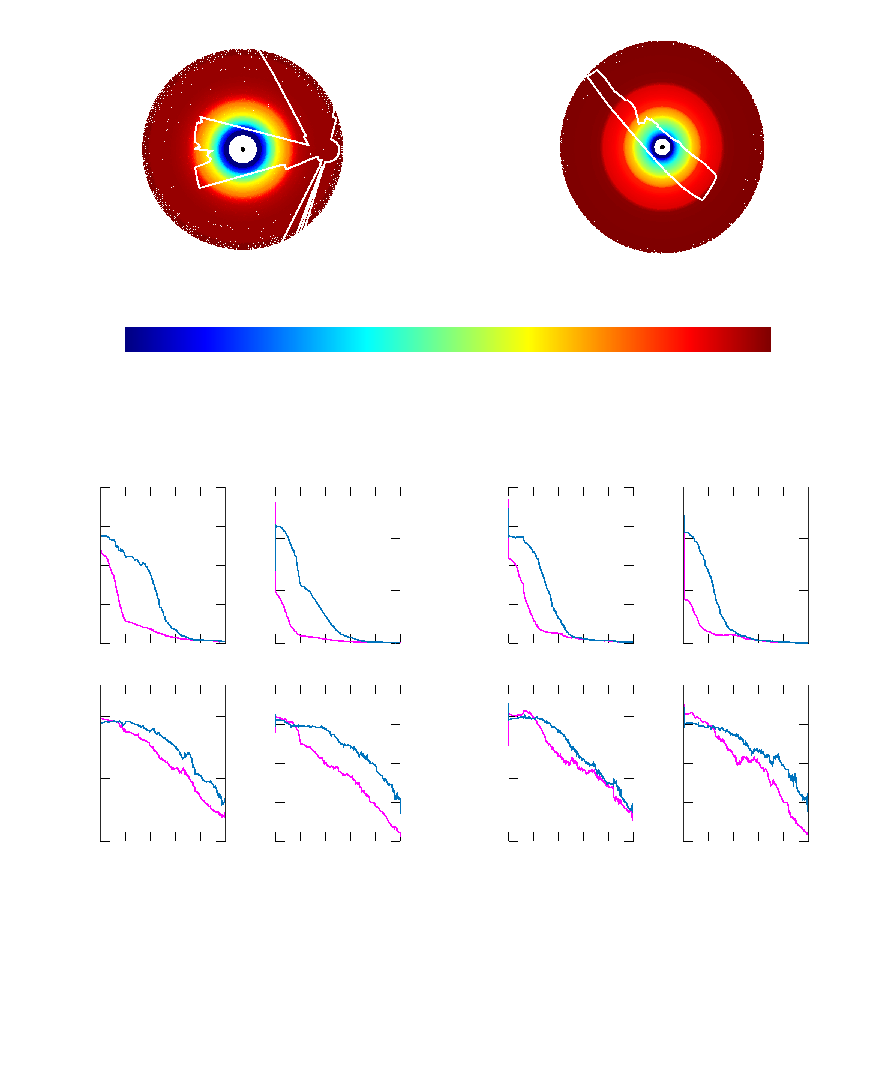
\includegraphics{./figures/parts/02/chapters/05/sections/04/max_range_test}}%
    \gplfronttext
  \end{picture}%
\endgroup

  \vspace{-2cm}
  \caption{\small Πειράματα απόκρισης του σφάλματος εκτίμησης των PLICP
           και FSM σε συνθήκες μειούμενου βεληνεκούς-μέγιστου εύρους
           για τυπική απόκλιση των διαταραχών που επιδρούν στις μετρήσεις του
           φυσικού αισθητήρα όταν $\sigma_R = 0.05$ m. Η διαμόρφωση
           $\Delta_\alpha: (\overline{\delta}_{xy}, \overline{\delta}_{\theta})
           = (0.05,0.174)$ [m,rad]. Η διαμόρφωση $\Delta_\beta:
           (\overline{\delta}_{xy},\overline{\delta}_{\theta}) = (0.20,\pi/4)$
           [m,rad]}
  \label{fig:02_05_04:03}
\end{figure}

Με βάση τα πειραματικά αποτελέσματα παρατηρούμε πως το σφάλμα εκτίμησης
προσανατολισμού του FSM είναι συγκρίσιμο με το ονομαστικό σε συνθήκες
όπου έως το $80\%$ των ακτίνων δεν φέρουν χωρική πληροφορία, σε αντίθεση με το
σφάλμα εκτίμησης θέσης, το οποίο είναι επί της αρχής αντιστρόφως ανάλογο του
ποσοστού των ακτίνων που φέρουν χωρική πληροφορία. Σε χαμηλότερα ποσοστά του
$80\%$ ο FSM επιδεικνύει χαμηλότερα σφάλματα εκτίμησης προσανατολισμού
από τον PLICP, ενώ τα σφάλματα εκτίμησης θέσης του γίνονται μεγαλύτερα από
εκείνα του PLICP όταν περίπου μόνο το $20\%$ των ακτίνων φέρουν ουσιαστική
πληροφορία, παρ' όλο που ο PLICP χρησιμοποιεί αντιστοιχίσεις (και συνεπώς θα
ήταν περισσότερο λογικό να είναι ικανός να αντιστοιχίσει μεμονωμένες περιοχές
των σαρώσεων μεταξύ τους).

Στο σχήμα \ref{fig:02_05_04:04} απεικονίζονται διαφορετικές όψεις της ευρωστίας
της μεθόδου FSM σε πραγματικές συνθήκες. Τα σχήματα της άνω σειράς
αναπαριστούν δύο αρχικές συνθήκες ευθυγράμμισης δισδιάστατων πανοραμικών
σαρώσεων, ενώ της μεσαίας τις τελικές ευθυγραμμίσεις που προέκυψαν μέσω της
εφαρμογής της FSM. Στην αριστερή συνθήκη η τυπική απόκλιση του θορύβου
μέτρησης είναι $\sigma_R = 0.05$ m, ενώ στη δεξιά $\sigma_R = 0.0$ m. Η
τελευταία σειρά εστιάζει σε σημεία ενδιαφέροντος, ήτοι σε περιοχές που εκθέτουν
την ευρωστία της μεθόδου ως προς το θόρυβο μέτρησης, αλλαγές περιβάλλοντος
απρόβλεπτου μέτρου, και ατελείς επικαλύψεις ανάμεσα στις εισόδους.

\begin{figure}[]\centering
  % GNUPLOT: LaTeX picture with Postscript
\begingroup
  \makeatletter
  \providecommand\color[2][]{%
    \GenericError{(gnuplot) \space\space\space\@spaces}{%
      Package color not loaded in conjunction with
      terminal option `colourtext'%
    }{See the gnuplot documentation for explanation.%
    }{Either use 'blacktext' in gnuplot or load the package
      color.sty in LaTeX.}%
    \renewcommand\color[2][]{}%
  }%
  \providecommand\includegraphics[2][]{%
    \GenericError{(gnuplot) \space\space\space\@spaces}{%
      Package graphicx or graphics not loaded%
    }{See the gnuplot documentation for explanation.%
    }{The gnuplot epslatex terminal needs graphicx.sty or graphics.sty.}%
    \renewcommand\includegraphics[2][]{}%
  }%
  \providecommand\rotatebox[2]{#2}%
  \@ifundefined{ifGPcolor}{%
    \newif\ifGPcolor
    \GPcolorfalse
  }{}%
  \@ifundefined{ifGPblacktext}{%
    \newif\ifGPblacktext
    \GPblacktexttrue
  }{}%
  % define a \g@addto@macro without @ in the name:
  \let\gplgaddtomacro\g@addto@macro
  % define empty templates for all commands taking text:
  \gdef\gplbacktext{}%
  \gdef\gplfronttext{}%
  \makeatother
  \ifGPblacktext
    % no textcolor at all
    \def\colorrgb#1{}%
    \def\colorgray#1{}%
  \else
    % gray or color?
    \ifGPcolor
      \def\colorrgb#1{\color[rgb]{#1}}%
      \def\colorgray#1{\color[gray]{#1}}%
      \expandafter\def\csname LTw\endcsname{\color{white}}%
      \expandafter\def\csname LTb\endcsname{\color{black}}%
      \expandafter\def\csname LTa\endcsname{\color{black}}%
      \expandafter\def\csname LT0\endcsname{\color[rgb]{1,0,0}}%
      \expandafter\def\csname LT1\endcsname{\color[rgb]{0,1,0}}%
      \expandafter\def\csname LT2\endcsname{\color[rgb]{0,0,1}}%
      \expandafter\def\csname LT3\endcsname{\color[rgb]{1,0,1}}%
      \expandafter\def\csname LT4\endcsname{\color[rgb]{0,1,1}}%
      \expandafter\def\csname LT5\endcsname{\color[rgb]{1,1,0}}%
      \expandafter\def\csname LT6\endcsname{\color[rgb]{0,0,0}}%
      \expandafter\def\csname LT7\endcsname{\color[rgb]{1,0.3,0}}%
      \expandafter\def\csname LT8\endcsname{\color[rgb]{0.5,0.5,0.5}}%
    \else
      % gray
      \def\colorrgb#1{\color{black}}%
      \def\colorgray#1{\color[gray]{#1}}%
      \expandafter\def\csname LTw\endcsname{\color{white}}%
      \expandafter\def\csname LTb\endcsname{\color{black}}%
      \expandafter\def\csname LTa\endcsname{\color{black}}%
      \expandafter\def\csname LT0\endcsname{\color{black}}%
      \expandafter\def\csname LT1\endcsname{\color{black}}%
      \expandafter\def\csname LT2\endcsname{\color{black}}%
      \expandafter\def\csname LT3\endcsname{\color{black}}%
      \expandafter\def\csname LT4\endcsname{\color{black}}%
      \expandafter\def\csname LT5\endcsname{\color{black}}%
      \expandafter\def\csname LT6\endcsname{\color{black}}%
      \expandafter\def\csname LT7\endcsname{\color{black}}%
      \expandafter\def\csname LT8\endcsname{\color{black}}%
    \fi
  \fi
    \setlength{\unitlength}{0.0500bp}%
    \ifx\gptboxheight\undefined%
      \newlength{\gptboxheight}%
      \newlength{\gptboxwidth}%
      \newsavebox{\gptboxtext}%
    \fi%
    \setlength{\fboxrule}{0.5pt}%
    \setlength{\fboxsep}{1pt}%
\begin{picture}(8000.00,12000.00)%
    \gplgaddtomacro\gplbacktext{%
      \colorrgb{0.15,0.15,0.15}%
      \put(-52,9611){\makebox(0,0)[r]{\strut{}$-32$}}%
      \colorrgb{0.15,0.15,0.15}%
      \put(-52,10173){\makebox(0,0)[r]{\strut{}$-24$}}%
      \colorrgb{0.15,0.15,0.15}%
      \put(-52,10734){\makebox(0,0)[r]{\strut{}$-16$}}%
      \colorrgb{0.15,0.15,0.15}%
      \put(-52,11296){\makebox(0,0)[r]{\strut{}$-8$}}%
      \colorrgb{0.15,0.15,0.15}%
      \put(-52,11857){\makebox(0,0)[r]{\strut{}$0$}}%
      \colorrgb{0.15,0.15,0.15}%
      \put(641,9321){\makebox(0,0){\strut{}$30$}}%
      \colorrgb{0.15,0.15,0.15}%
      \put(1343,9321){\makebox(0,0){\strut{}$50$}}%
      \colorrgb{0.15,0.15,0.15}%
      \put(2045,9321){\makebox(0,0){\strut{}$50$}}%
      \colorrgb{0.15,0.15,0.15}%
      \put(2746,9321){\makebox(0,0){\strut{}$60$}}%
      \colorrgb{0.15,0.15,0.15}%
      \put(3448,9321){\makebox(0,0){\strut{}$70$}}%
    }%
    \gplgaddtomacro\gplfronttext{%
      \colorrgb{0.00,0.00,0.00}%
      \put(1182,12050){\makebox(0,0)[l]{\strut{}Αρχική συνθήκη}}%
      \put(982,9000){\makebox(0,0)[l]{\strut{}$\Delta x = -0.03252$ m}}%
      \put(982,8750){\makebox(0,0)[l]{\strut{}$\Delta y = +0.03603$ m}}%
      \put(982,8500){\makebox(0,0)[l]{\strut{}$\Delta \theta = -0.35689$ rad}}%
    }%
    \gplgaddtomacro\gplbacktext{%
      \colorrgb{0.15,0.15,0.15}%
      \put(4748,9755){\makebox(0,0)[r]{\strut{}$-12$}}%
      \colorrgb{0.15,0.15,0.15}%
      \put(4748,10227){\makebox(0,0)[r]{\strut{}$-10$}}%
      \colorrgb{0.15,0.15,0.15}%
      \put(4748,10699){\makebox(0,0)[r]{\strut{}$-8$}}%
      \colorrgb{0.15,0.15,0.15}%
      \put(4748,11171){\makebox(0,0)[r]{\strut{}$-6$}}%
      \colorrgb{0.15,0.15,0.15}%
      \put(4748,11643){\makebox(0,0)[r]{\strut{}$-4$}}%
      \colorrgb{0.15,0.15,0.15}%
      \put(5116,9299){\makebox(0,0){\strut{}$28$}}%
      \colorrgb{0.15,0.15,0.15}%
      \put(5588,9299){\makebox(0,0){\strut{}$30$}}%
      \colorrgb{0.15,0.15,0.15}%
      \put(6060,9299){\makebox(0,0){\strut{}$32$}}%
      \colorrgb{0.15,0.15,0.15}%
      \put(6531,9299){\makebox(0,0){\strut{}$34$}}%
      \colorrgb{0.15,0.15,0.15}%
      \put(7003,9299){\makebox(0,0){\strut{}$36$}}%
    }%
    \gplgaddtomacro\gplfronttext{%
      \colorrgb{0.00,0.00,0.00}%
      \put(5300,12050){\makebox(0,0)[l]{\strut{}Αρχική συνθήκη}}%
      \put(5200,9000){\makebox(0,0)[l]{\strut{}$\Delta x = -0.02856$ m}}%
      \put(5200,8750){\makebox(0,0)[l]{\strut{}$\Delta y = -0.19805$ m}}%
      \put(5200,8500){\makebox(0,0)[l]{\strut{}$\Delta \theta = -1.31500$ rad}}%
    }%
    \gplgaddtomacro\gplbacktext{%
      \colorrgb{0.15,0.15,0.15}%
      \put(-52,6118){\makebox(0,0)[r]{\strut{}$-32$}}%
      \colorrgb{0.15,0.15,0.15}%
      \put(-52,6399){\makebox(0,0)[r]{\strut{}$-28$}}%
      \colorrgb{0.15,0.15,0.15}%
      \put(-52,6679){\makebox(0,0)[r]{\strut{}$-24$}}%
      \colorrgb{0.15,0.15,0.15}%
      \put(-52,6960){\makebox(0,0)[r]{\strut{}$-20$}}%
      \colorrgb{0.15,0.15,0.15}%
      \put(641,5828){\makebox(0,0){\strut{}$30$}}%
      \colorrgb{0.15,0.15,0.15}%
      \put(1343,5828){\makebox(0,0){\strut{}$50$}}%
      \colorrgb{0.15,0.15,0.15}%
      \put(2045,5828){\makebox(0,0){\strut{}$50$}}%
      \colorrgb{0.15,0.15,0.15}%
      \put(2746,5828){\makebox(0,0){\strut{}$60$}}%
      \colorrgb{0.15,0.15,0.15}%
      \put(3448,5828){\makebox(0,0){\strut{}$70$}}%
    }%
    \gplgaddtomacro\gplfronttext{%
      \colorrgb{0.00,0.00,0.00}%
      \put(982,7200){\makebox(0,0)[l]{\strut{}Τελική ευθυγράμμιση}}%
      \put(982,5500){\makebox(0,0)[l]{\strut{}$\Delta x = -0.00085$ m}}%
      \put(982,5250){\makebox(0,0)[l]{\strut{}$\Delta y = +0.00337$ m}}%
      \put(982,5000){\makebox(0,0)[l]{\strut{}$\Delta \theta = -0.00346$ rad}}%
    }%
    \gplgaddtomacro\gplbacktext{%
      \colorrgb{0.15,0.15,0.15}%
      \put(4748,5596){\makebox(0,0)[r]{\strut{}$-12$}}%
      \colorrgb{0.15,0.15,0.15}%
      \put(4748,6068){\makebox(0,0)[r]{\strut{}$-10$}}%
      \colorrgb{0.15,0.15,0.15}%
      \put(4748,6540){\makebox(0,0)[r]{\strut{}$-8$}}%
      \colorrgb{0.15,0.15,0.15}%
      \put(4748,7011){\makebox(0,0)[r]{\strut{}$-6$}}%
      \colorrgb{0.15,0.15,0.15}%
      \put(4748,7483){\makebox(0,0)[r]{\strut{}$-4$}}%
      \colorrgb{0.15,0.15,0.15}%
      \put(5116,5140){\makebox(0,0){\strut{}$28$}}%
      \colorrgb{0.15,0.15,0.15}%
      \put(5588,5140){\makebox(0,0){\strut{}$30$}}%
      \colorrgb{0.15,0.15,0.15}%
      \put(6060,5140){\makebox(0,0){\strut{}$32$}}%
      \colorrgb{0.15,0.15,0.15}%
      \put(6531,5140){\makebox(0,0){\strut{}$34$}}%
      \colorrgb{0.15,0.15,0.15}%
      \put(7003,5140){\makebox(0,0){\strut{}$36$}}%
    }%
    \gplgaddtomacro\gplfronttext{%
      \colorrgb{0.00,0.00,0.00}%
      \put(5100,7900){\makebox(0,0)[l]{\strut{}Τελική ευθυγράμμιση}}%
      \put(5200,4800){\makebox(0,0)[l]{\strut{}$\Delta x = +0.00643$ m}}%
      \put(5200,4550){\makebox(0,0)[l]{\strut{}$\Delta y = +0.00371$ m}}%
      \put(5200,4300){\makebox(0,0)[l]{\strut{}$\Delta \theta = +0.00194$ rad}}%
    }%
    \gplgaddtomacro\gplbacktext{%
      \colorrgb{0.15,0.15,0.15}%
      \put(42,1815){\makebox(0,0)[r]{\strut{}\scriptsize $-26$}}%
      \colorrgb{0.15,0.15,0.15}%
      \put(42,2479){\makebox(0,0)[r]{\strut{}\scriptsize $-25$}}%
      \colorrgb{0.15,0.15,0.15}%
      \put(42,3143){\makebox(0,0)[r]{\strut{}\scriptsize $-24$}}%
      \colorrgb{0.15,0.15,0.15}%
      \put(412,1263){\makebox(0,0){\strut{}\scriptsize $26$}}%
      \colorrgb{0.15,0.15,0.15}%
      \put(1075,1263){\makebox(0,0){\strut{}\scriptsize $27$}}%
      \colorrgb{0.15,0.15,0.15}%
      \put(1739,1263){\makebox(0,0){\strut{}\scriptsize $28$}}%
    }%
    \gplgaddtomacro\gplfronttext{%
      \colorrgb{0.00,0.00,0.00}%
      \put(909,3496){\makebox(0,0){\strut{}Θόρυβος μέτρησης}}%
    }%
    \gplgaddtomacro\gplbacktext{%
      \colorrgb{0.15,0.15,0.15}%
      \put(2108,2073){\makebox(0,0)[r]{\strut{}\scriptsize $-25$}}%
      \colorrgb{0.15,0.15,0.15}%
      \put(2108,2364){\makebox(0,0)[r]{\strut{}\scriptsize $-24$}}%
      \colorrgb{0.15,0.15,0.15}%
      \put(2108,2656){\makebox(0,0)[r]{\strut{}\scriptsize $-23$}}%
      \colorrgb{0.15,0.15,0.15}%
      \put(2518,1635){\makebox(0,0){\strut{}\scriptsize $31$}}%
      \colorrgb{0.15,0.15,0.15}%
      \put(3100,1635){\makebox(0,0){\strut{}\scriptsize $33$}}%
      \colorrgb{0.15,0.15,0.15}%
      \put(3683,1635){\makebox(0,0){\strut{}\scriptsize $35$}}%
    }%
    \gplgaddtomacro\gplfronttext{%
    }%
    \gplgaddtomacro\gplbacktext{%
      \colorrgb{0.15,0.15,0.15}%
      \put(4168,1901){\makebox(0,0)[r]{\strut{}\scriptsize $-6$}}%
      \colorrgb{0.15,0.15,0.15}%
      \put(4168,2464){\makebox(0,0)[r]{\strut{}\scriptsize $-5$}}%
      \colorrgb{0.15,0.15,0.15}%
      \put(4168,3027){\makebox(0,0)[r]{\strut{}\scriptsize $-4$}}%
      \colorrgb{0.15,0.15,0.15}%
      \put(4706,1231){\makebox(0,0){\strut{}\scriptsize $32$}}%
      \colorrgb{0.15,0.15,0.15}%
      \put(5269,1231){\makebox(0,0){\strut{}\scriptsize $33$}}%
      \colorrgb{0.15,0.15,0.15}%
      \put(5831,1231){\makebox(0,0){\strut{}\scriptsize $34$}}%
    }%
    \gplgaddtomacro\gplfronttext{%
      \colorrgb{0.00,0.00,0.00}%
      \put(2457,3589){\makebox(0,0)[l]{\strut{}Στοιχεία υψηλής συχνότητος}}%
    }%
    \gplgaddtomacro\gplbacktext{%
      \colorrgb{0.15,0.15,0.15}%
      \put(6228,1704){\makebox(0,0)[r]{\strut{}\scriptsize $-8$}}%
      \colorrgb{0.15,0.15,0.15}%
      \put(6228,2165){\makebox(0,0)[r]{\strut{}\scriptsize $-7$}}%
      \colorrgb{0.15,0.15,0.15}%
      \put(6228,2626){\makebox(0,0)[r]{\strut{}\scriptsize $-6$}}%
      \colorrgb{0.15,0.15,0.15}%
      \put(6228,3087){\makebox(0,0)[r]{\strut{}\scriptsize $-5$}}%
      \colorrgb{0.15,0.15,0.15}%
      \put(6260,1406){\makebox(0,0){\strut{}\scriptsize $30$}}%
      \colorrgb{0.15,0.15,0.15}%
      \put(6721,1406){\makebox(0,0){\strut{}\scriptsize $31$}}%
      \colorrgb{0.15,0.15,0.15}%
      \put(7182,1406){\makebox(0,0){\strut{}\scriptsize $32$}}%
      \colorrgb{0.15,0.15,0.15}%
      \put(7643,1406){\makebox(0,0){\strut{}\scriptsize $33$}}%
    }%
    \gplgaddtomacro\gplfronttext{%
      \colorrgb{0.00,0.00,0.00}%
      \put(7089,3353){\makebox(0,0){\strut{}Απούσες αντιστοιχίες}}%
    }%
    \gplbacktext
    \put(0,0){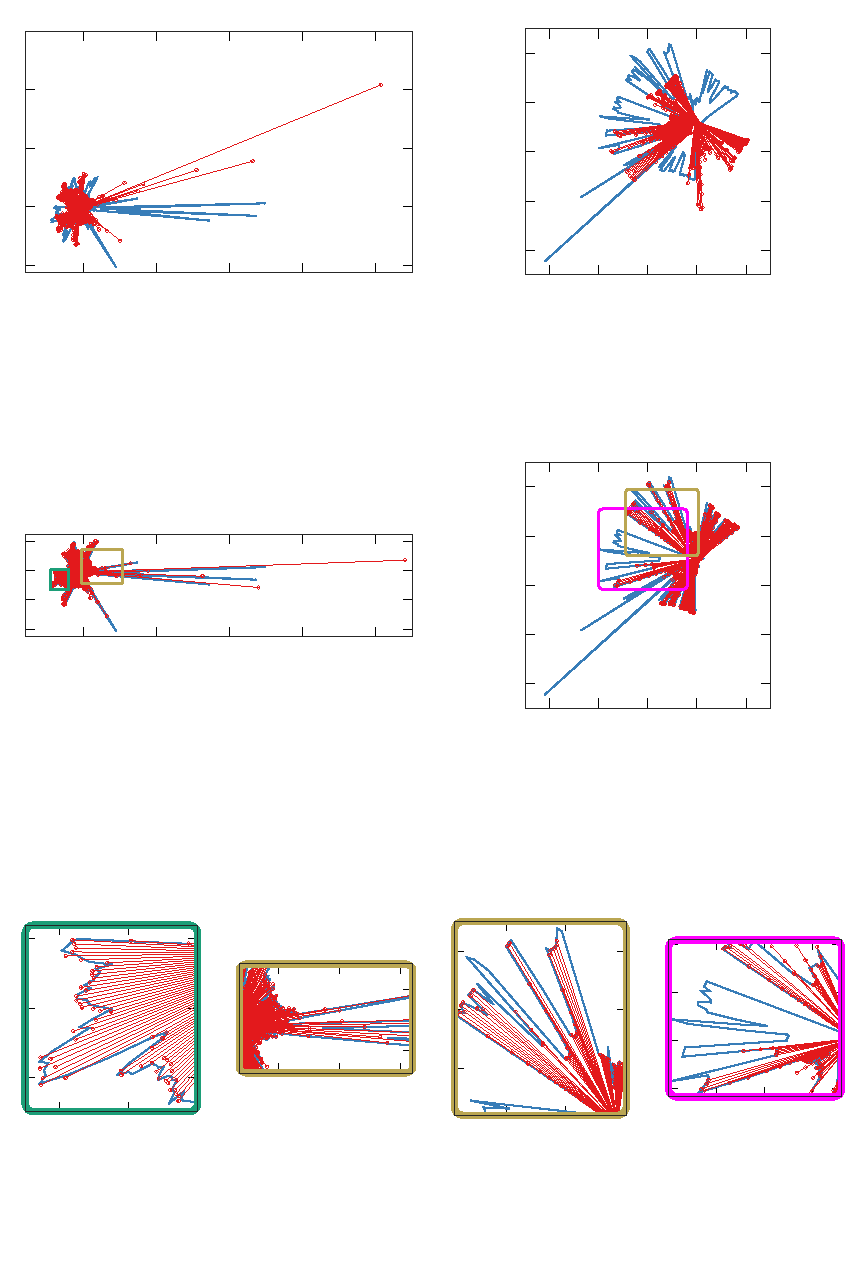
\includegraphics{./figures/parts/02/chapters/05/sections/04/from_video}}%
    \gplfronttext
  \end{picture}%
\endgroup

  \vspace{-1cm}
  \caption{\small Παραδείγματα ευθυγράμμισης σαρώσεων που εκθέτουν τις αρετές
           του FSM σε καταστάσεις πραγματικών συνθηκών: ο FSM
           είναι ταυτόχρονα εύρωστος σε θόρυβο μέτρησης, απρόβλεπτα μεγάλες
           αλλαγές στο περιβάλλον από το οποίο συλλαμβάνονται οι σαρώσεις
           εισόδου του, και σε συνθήκες μερικής επικάλυψης}
  \label{fig:02_05_04:04}
\end{figure}


%%%%%%%%%%%%%%%%%%%%%%%%%%%%%%%%%%%%%%%%%%%%%%%%%%%%%%%%%%%%%%%%%%%%%%%%%%%%%%%%
\section{Συμπεράσματα και περαιτέρω έρευνα}
  \label{section:02_03_05}
  %%%%%%%%%%%%%%%%%%%%%%%%%%%%%%%%%%%%%%%%%%%%%%%%%%%%%%%%%%%%%%%%%%%%%%%%%%%%%%%%
\subsection{Συμπεράσματα κεφαλαίου}
\label{subsection:02_01_05:01}

Σε αυτό το κεφάλαιο αξιολογήσαμε την επίδοση των τελευταίας τεχνολογίας πακέτων
λογισμικού ROS που είναι ικανά να φέρουν εις πέρας το έργο της αυτόνομους
πλοήγησης στο πεδίο εφαρμογής \ref{scope}. Οι αλγόριθμοι αυτοί είναι δύο ειδών:
αλγόριθμοι χάραξης μονοπατιών ανάμεσα σε δύο στάσεις του χάρτη του περιβάλλοντος
στο οποίο κινείται μία κινητή βάση ρομπότ, και αλγόριθμοι ελέγχου της κίνησης
του ρομπότ στο περιβάλλον του. Ο συνδυασμός τους αποτελεί τον πυρήνα της
πλοήγησης μίας κινητής βάσης ρομπότ άνευ εξωτερικών χειροκίνητων χειρισμών της.

Η αξιολόγηση είχε ως στόχους
\begin{itemize}
  \item το σχεδιασμό μίας ολοκληρωμένης, περιεκτικής, και επεκτάσιμης
        μεθοδολογίας αξιολόγησης μεθόδων αυτόνομους πλοήγησης κινητών βάσεων
        ρομπότ, και
  \item την εφαρμογή της για την αξιολόγηση της επίδοσης τρεχόντων υλοποιήσεών
        τους μέσω του μεσολογισμικού ROS
\end{itemize}

Προκειμένου να διακρίνουμε τα εύρωστα και εύχρηστα πακέτα λογισμικού από τα μη,
συστήσαμε μία μεθοδολογία προκαταρκτικής αξιολόγησής τους με βάσει ποιοτικά
κριτήρια που τίθενται από την εμπειρία ανάπτυξης και συντήρησης λογισμικού.
Στη συνέχεια σχεδιάσαμε μία μεθοδολογία αξιολόγησης με βάση ποσοτικές μετρικές,
οι οποίες αποτελούν αντικειμενικά κριτήρια της επίδοσης ενός ρομπότ στο έργο
της αυτόνομους πλοήγησης, και στις οποίες ένας μηχανικός ρομποτικής μπορεί να
θέσει επιπλέον ή λιγότερο βάρος αναλόγως των σκοπών της εφαρμογής των εν λόγω
πακέτων αυτόνομους πλοήγησης. Έπειτα εφαρμόσαμε τη μεθοδολογία ποσοτικής
αξιολόγησης σε εννιά συνδυασμούς πακέτων, πραγματοποιώντας χρήση τους για
αυτόνομη πλοήγηση σε δύο ετερογενή προσομοιωμένα περιβάλλοντα και σε ένα
πραγματικό. Τα περιβάλλοντα και οι διαδρομές πλοήγησης επιλέχθηκαν έτσι ώστε
να δοκιμάσουν τους υποκείμενους αλγορίθμους με μία σειρά κριτηρίων, και με
κλιμακωτή δυσκολία. Το αποτέλεσμα ήταν μία ιεράρχηση των συνδυασμών των πακέτων
λογισμικού, στην κορυφή της οποίας βρίσκεται ένας συνδυασμός ο οποίος φέρει
εις πέρας το έργο της αυτόνομους πλοήγησης με ελάχιστα σφάλματα πλοήγησης,
σε εύλογους χρόνους, και, συνολικά, άριστη επίδοση στο σύνολο των τριών
περιβαλλόντων δοκιμής.


%%%%%%%%%%%%%%%%%%%%%%%%%%%%%%%%%%%%%%%%%%%%%%%%%%%%%%%%%%%%%%%%%%%%%%%%%%%%%%%%
\subsection{Αιτίες περαιτέρω έρευνας}
\label{subsection:02_01_05:02}

Για το σκοπό της αυτόνομους πλοήγησης είναι απαραίτητη η γνώση ή η εκτίμηση της
τρέχουσας στάσης του ρομπότ: μόνο με βάση αυτήν είναι δυνατή η εύρεση ταχυτήτων
προς είσοδο στους κινητήρες των τροχών της κινητής βάσης έτσι ώστε να
ακολουθείται το σχεδιασθέν μονοπάτι. Στο πεδίο εφαρμογής \ref{scope} η γνώση
της στάσης δεν είναι δυνατή: μόνο η παρατήρησή της είναι δυνατή, μέσω των
αισθητήρων που φέρει το ρομπότ (παρατήρηση \ref{remark:01}). Για την παρατήρηση
της στάσης του ρομπότ κατά τη διενέργεια της πειραματικής διαδικασίας
χρησιμοποιήσαμε το φίλτρο σωματιδίων (ενότητα \ref{subsec:01_01_02_3}).

Αυτό που παρατηρήσαμε δια ζώσης και με γυμνό μάτι κατά τη διάρκεια της
πειραματικής διαδικασίας ήταν ότι η εκτίμηση της στάσης του ρομπότ δεν σύναδε
πάντοτε με την πραγματική του στάση: σε λίγες περιπτώσεις παρατηρήσαμε ότι η
εκτίμηση της θέσης ταλαντωνόταν απότομα ανάμεσα σε μερικές υποψήφιες
θέσεις---σε άλλες στιγμές παρατηρούσαμε ότι η εκτίμηση της στάσης του ρομπότ
είχε ορατό σφάλμα σε σχέση με την πραγματική του στάση. Το σχήμα
\ref{fig:02_01_05} δείχνει την εξέλιξη του μέσου όρου των σφαλμάτων κατάστασης
(του διανύσματος της στάσης) κατά τις δέκα διαδρομές του συνδυασμού του ελεγκτή
\texttt{teb\_local\_planner} με τον αλγόριθμο χάραξης μονοπατιών \texttt{navfn}
στο περιβάλλον CORRIDOR (αριστερά) και με τον \texttt{global\_planner} στο
περιβάλλον WILLOWGARAGE (δεξιά). Σε αυτά τα σχήματα παρατηρούμε τέσσερα
πράγματα για το σφάλμα κατάστασης:
(α) δεν έχει σταθερά μηδενική (ή αμελητέα) τιμή,
(β) δεν έχει σταθερή τιμή μέσα στο χώρο και κατά τη διάρκεια του χρόνου,
(γ) δεν έχει παρόμοιες καμπύλες εξέλιξης σε διαφορετικά περιβάλλοντα, και
(δ) δεν έχει το ίδιο άνω ή κάτω όριο σε διαφορετικά περιβάλλοντα.\footnote{Από
την ανάλυση των αποτελεσμάτων για όλους τους συνδυασμούς αλγορίθμων χάραξης
μονοπατιών με ελεγκτές κίνησης προκύπτει, όπως είναι εύλογο, ότι το σφάλμα
κατάστασης είναι ανεξάρτητο από αυτούς.}

Ανάλογα με τους σκοπούς ρομποτικών εφαρμογών το σφάλμα κατάστασης μπορεί να
έχει μεταβλητές προδιαγραφές. Για παράδειγμα, σε αποθήκες με μεγάλους χώρους και
πλατειά περάσματα, όπου ο στόχος είναι η απογραφή της θέσης προϊόντων με αδρή
ακρίβεια θέσης (της τάξης των δεκάδων εκατοστών του μέτρου), ούτε η πλοήγηση
δυσχεραίνεται, ούτε και διαταράσσεται η ακρίβεια της απογραφής. Αντιθέτως,
σε περιβάλλοντα με στενά περάσματα ή απαιτήσεις ακριβείας στάσης (για παράδειγμα
σε αυτόνομα παλετοφόρα οχήματα), η αυτόνομη πλοήγηση δυσχεραίνεται σε αναλογία
με το σφάλμα στάσης και το πόσο στενά είναι τα περάσματα, και το έργο που
απαιτεί ακρίβεια στάσης του ρομπότ (η φόρτωση των παλετών από το όχημα) σε
αναλογία με το μέγεθος του σφάλματος στάσης. Στο πλαίσιο της βιομηχανίας η
ελάττωση του σφάλματος εκτίμησης της στάσης ενός αυτόνομου ρομπότ προς το παρόν
επιτυγχάνεται είτε με επιπρόσθετο και κοστοβόρο εξοπλισμό, είτε με την απόρριψη
της αυτονομίας λόγω των υψηλών διακυβευμάτων σε κόστος και ασφάλεια.

Η έρευνα επί της ελάττωσης του σφάλματος της εκτίμησης της στάσης ενός ρομπότ
στο πεδίο εφαρμογής \ref{scope} θα είναι επικερδής για τους σκοπούς της
διάχυσης της αυτονομίας, και σε υπάρχουσες εφαρμογές που απαιτούν αυξημένη
ακρίβεια εκτίμησης σε σχέση με τις συμβατικές προσεγγίσεις εκτίμησης της στάσης
ενός αυτόνομου ρομπότ στο χώρο.

\begin{figure}[h]\vspace{1cm}\centering
   \begin{subfigure}{0.49\linewidth}\centering
     % GNUPLOT: LaTeX picture with Postscript
\begingroup
  \makeatletter
  \providecommand\color[2][]{%
    \GenericError{(gnuplot) \space\space\space\@spaces}{%
      Package color not loaded in conjunction with
      terminal option `colourtext'%
    }{See the gnuplot documentation for explanation.%
    }{Either use 'blacktext' in gnuplot or load the package
      color.sty in LaTeX.}%
    \renewcommand\color[2][]{}%
  }%
  \providecommand\includegraphics[2][]{%
    \GenericError{(gnuplot) \space\space\space\@spaces}{%
      Package graphicx or graphics not loaded%
    }{See the gnuplot documentation for explanation.%
    }{The gnuplot epslatex terminal needs graphicx.sty or graphics.sty.}%
    \renewcommand\includegraphics[2][]{}%
  }%
  \providecommand\rotatebox[2]{#2}%
  \@ifundefined{ifGPcolor}{%
    \newif\ifGPcolor
    \GPcolorfalse
  }{}%
  \@ifundefined{ifGPblacktext}{%
    \newif\ifGPblacktext
    \GPblacktexttrue
  }{}%
  % define a \g@addto@macro without @ in the name:
  \let\gplgaddtomacro\g@addto@macro
  % define empty templates for all commands taking text:
  \gdef\gplfronttext{}%
  \gdef\gplfronttext{}%
  \makeatother
  \ifGPblacktext
    % no textcolor at all
    \def\colorrgb#1{}%
    \def\colorgray#1{}%
  \else
    % gray or color?
    \ifGPcolor
      \def\colorrgb#1{\color[rgb]{#1}}%
      \def\colorgray#1{\color[gray]{#1}}%
      \expandafter\def\csname LTw\endcsname{\color{white}}%
      \expandafter\def\csname LTb\endcsname{\color{black}}%
      \expandafter\def\csname LTa\endcsname{\color{black}}%
      \expandafter\def\csname LT0\endcsname{\color[rgb]{1,0,0}}%
      \expandafter\def\csname LT1\endcsname{\color[rgb]{0,1,0}}%
      \expandafter\def\csname LT2\endcsname{\color[rgb]{0,0,1}}%
      \expandafter\def\csname LT3\endcsname{\color[rgb]{1,0,1}}%
      \expandafter\def\csname LT4\endcsname{\color[rgb]{0,1,1}}%
      \expandafter\def\csname LT5\endcsname{\color[rgb]{1,1,0}}%
      \expandafter\def\csname LT6\endcsname{\color[rgb]{0,0,0}}%
      \expandafter\def\csname LT7\endcsname{\color[rgb]{1,0.3,0}}%
      \expandafter\def\csname LT8\endcsname{\color[rgb]{0.5,0.5,0.5}}%
    \else
      % gray
      \def\colorrgb#1{\color{black}}%
      \def\colorgray#1{\color[gray]{#1}}%
      \expandafter\def\csname LTw\endcsname{\color{white}}%
      \expandafter\def\csname LTb\endcsname{\color{black}}%
      \expandafter\def\csname LTa\endcsname{\color{black}}%
      \expandafter\def\csname LT0\endcsname{\color{black}}%
      \expandafter\def\csname LT1\endcsname{\color{black}}%
      \expandafter\def\csname LT2\endcsname{\color{black}}%
      \expandafter\def\csname LT3\endcsname{\color{black}}%
      \expandafter\def\csname LT4\endcsname{\color{black}}%
      \expandafter\def\csname LT5\endcsname{\color{black}}%
      \expandafter\def\csname LT6\endcsname{\color{black}}%
      \expandafter\def\csname LT7\endcsname{\color{black}}%
      \expandafter\def\csname LT8\endcsname{\color{black}}%
    \fi
  \fi
  \setlength{\unitlength}{0.0500bp}%
  \begin{picture}(4000.00,3200.00)%
    \gplgaddtomacro\gplfronttext{%
      \colorrgb{0.00,0.00,0.00}%
      \put(726,440){\makebox(0,0)[r]{\strut{}$0.0$}}%
      \colorrgb{0.00,0.00,0.00}%
      \put(726,752){\makebox(0,0)[r]{\strut{}$0.01$}}%
      \colorrgb{0.00,0.00,0.00}%
      \put(726,1064){\makebox(0,0)[r]{\strut{}$0.02$}}%
      \colorrgb{0.00,0.00,0.00}%
      \put(726,1376){\makebox(0,0)[r]{\strut{}$0.03$}}%
      \colorrgb{0.00,0.00,0.00}%
      \put(726,1688){\makebox(0,0)[r]{\strut{}$0.04$}}%
      \colorrgb{0.00,0.00,0.00}%
      \put(726,1999){\makebox(0,0)[r]{\strut{}$0.05$}}%
      \colorrgb{0.00,0.00,0.00}%
      \put(726,2311){\makebox(0,0)[r]{\strut{}$0.06$}}%
      \colorrgb{0.00,0.00,0.00}%
      \put(726,2623){\makebox(0,0)[r]{\strut{}$0.07$}}%
      \colorrgb{0.00,0.00,0.00}%
      \put(726,2935){\makebox(0,0)[r]{\strut{}$0.08$}}%
      \colorrgb{0.00,0.00,0.00}%
      \put(858,220){\makebox(0,0){\strut{}$0$}}%
      \colorrgb{0.00,0.00,0.00}%
      \put(1316,220){\makebox(0,0){\strut{}$20$}}%
      \colorrgb{0.00,0.00,0.00}%
      \put(1773,220){\makebox(0,0){\strut{}$40$}}%
      \colorrgb{0.00,0.00,0.00}%
      \put(2231,220){\makebox(0,0){\strut{}$60$}}%
      \colorrgb{0.00,0.00,0.00}%
      \put(2688,220){\makebox(0,0){\strut{}$80$}}%
      \colorrgb{0.00,0.00,0.00}%
      \put(3146,220){\makebox(0,0){\strut{}$100$}}%
      \colorrgb{0.00,0.00,0.00}%
      \put(3603,220){\makebox(0,0){\strut{}$120$}}%
      \put(4400,3420){\makebox(0,0){\strut{}Σφάλμα κατάστασης $[(\text{m}^2 + \text{rad}^2)^{1/2}]$}}%
      \put(4400,-200){\makebox(0,0){\strut{}Αριθμός εκτιμήσεων στάσης στο χρόνο}}%
    }%
    \gplgaddtomacro\gplfronttext{%
    }%
    \gplfronttext
    \put(0,0){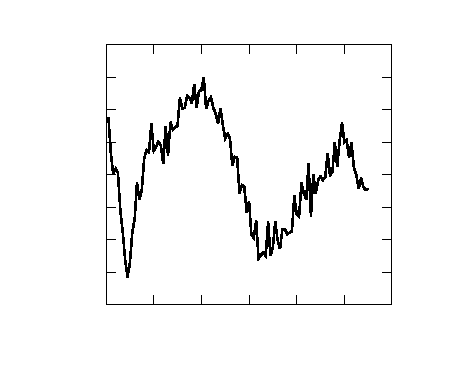
\includegraphics{./figures/parts/02/chapters/01/sections/05/pose_navfn_corridor}}%
    \gplfronttext
  \end{picture}%
\endgroup

     \vspace{0.75cm}
     \caption{\small CORRIDOR}
   \end{subfigure}
   \begin{subfigure}{0.49\linewidth} \centering
     % GNUPLOT: LaTeX picture with Postscript
\begingroup
  \makeatletter
  \providecommand\color[2][]{%
    \GenericError{(gnuplot) \space\space\space\@spaces}{%
      Package color not loaded in conjunction with
      terminal option `colourtext'%
    }{See the gnuplot documentation for explanation.%
    }{Either use 'blacktext' in gnuplot or load the package
      color.sty in LaTeX.}%
    \renewcommand\color[2][]{}%
  }%
  \providecommand\includegraphics[2][]{%
    \GenericError{(gnuplot) \space\space\space\@spaces}{%
      Package graphicx or graphics not loaded%
    }{See the gnuplot documentation for explanation.%
    }{The gnuplot epslatex terminal needs graphicx.sty or graphics.sty.}%
    \renewcommand\includegraphics[2][]{}%
  }%
  \providecommand\rotatebox[2]{#2}%
  \@ifundefined{ifGPcolor}{%
    \newif\ifGPcolor
    \GPcolorfalse
  }{}%
  \@ifundefined{ifGPblacktext}{%
    \newif\ifGPblacktext
    \GPblacktexttrue
  }{}%
  % define a \g@addto@macro without @ in the name:
  \let\gplgaddtomacro\g@addto@macro
  % define empty templates for all commands taking text:
  \gdef\gplfronttext{}%
  \gdef\gplfronttext{}%
  \makeatother
  \ifGPblacktext
    % no textcolor at all
    \def\colorrgb#1{}%
    \def\colorgray#1{}%
  \else
    % gray or color?
    \ifGPcolor
      \def\colorrgb#1{\color[rgb]{#1}}%
      \def\colorgray#1{\color[gray]{#1}}%
      \expandafter\def\csname LTw\endcsname{\color{white}}%
      \expandafter\def\csname LTb\endcsname{\color{black}}%
      \expandafter\def\csname LTa\endcsname{\color{black}}%
      \expandafter\def\csname LT0\endcsname{\color[rgb]{1,0,0}}%
      \expandafter\def\csname LT1\endcsname{\color[rgb]{0,1,0}}%
      \expandafter\def\csname LT2\endcsname{\color[rgb]{0,0,1}}%
      \expandafter\def\csname LT3\endcsname{\color[rgb]{1,0,1}}%
      \expandafter\def\csname LT4\endcsname{\color[rgb]{0,1,1}}%
      \expandafter\def\csname LT5\endcsname{\color[rgb]{1,1,0}}%
      \expandafter\def\csname LT6\endcsname{\color[rgb]{0,0,0}}%
      \expandafter\def\csname LT7\endcsname{\color[rgb]{1,0.3,0}}%
      \expandafter\def\csname LT8\endcsname{\color[rgb]{0.5,0.5,0.5}}%
    \else
      % gray
      \def\colorrgb#1{\color{black}}%
      \def\colorgray#1{\color[gray]{#1}}%
      \expandafter\def\csname LTw\endcsname{\color{white}}%
      \expandafter\def\csname LTb\endcsname{\color{black}}%
      \expandafter\def\csname LTa\endcsname{\color{black}}%
      \expandafter\def\csname LT0\endcsname{\color{black}}%
      \expandafter\def\csname LT1\endcsname{\color{black}}%
      \expandafter\def\csname LT2\endcsname{\color{black}}%
      \expandafter\def\csname LT3\endcsname{\color{black}}%
      \expandafter\def\csname LT4\endcsname{\color{black}}%
      \expandafter\def\csname LT5\endcsname{\color{black}}%
      \expandafter\def\csname LT6\endcsname{\color{black}}%
      \expandafter\def\csname LT7\endcsname{\color{black}}%
      \expandafter\def\csname LT8\endcsname{\color{black}}%
    \fi
  \fi
  \setlength{\unitlength}{0.0500bp}%
  \begin{picture}(4000.00,3200.00)%
    \gplgaddtomacro\gplfronttext{%
      \colorrgb{0.00,0.00,0.00}%
      \put(726,440){\makebox(0,0)[r]{\strut{}$0.0$}}%
      \colorrgb{0.00,0.00,0.00}%
      \put(726,796){\makebox(0,0)[r]{\strut{}$0.05$}}%
      \colorrgb{0.00,0.00,0.00}%
      \put(726,1153){\makebox(0,0)[r]{\strut{}$0.10$}}%
      \colorrgb{0.00,0.00,0.00}%
      \put(726,1509){\makebox(0,0)[r]{\strut{}$0.15$}}%
      \colorrgb{0.00,0.00,0.00}%
      \put(726,1866){\makebox(0,0)[r]{\strut{}$0.20$}}%
      \colorrgb{0.00,0.00,0.00}%
      \put(726,2222){\makebox(0,0)[r]{\strut{}$0.25$}}%
      \colorrgb{0.00,0.00,0.00}%
      \put(726,2579){\makebox(0,0)[r]{\strut{}$0.30$}}%
      \colorrgb{0.00,0.00,0.00}%
      \put(726,2935){\makebox(0,0)[r]{\strut{}$0.35$}}%
      \colorrgb{0.00,0.00,0.00}%
      \put(858,220){\makebox(0,0){\strut{}$0$}}%
      \colorrgb{0.00,0.00,0.00}%
      \put(1544,220){\makebox(0,0){\strut{}$50$}}%
      \colorrgb{0.00,0.00,0.00}%
      \put(2231,220){\makebox(0,0){\strut{}$100$}}%
      \colorrgb{0.00,0.00,0.00}%
      \put(2917,220){\makebox(0,0){\strut{}$150$}}%
      \colorrgb{0.00,0.00,0.00}%
      \put(3603,220){\makebox(0,0){\strut{}$200$}}%
    }%
    \gplgaddtomacro\gplfronttext{%
    }%
    \put(0,0){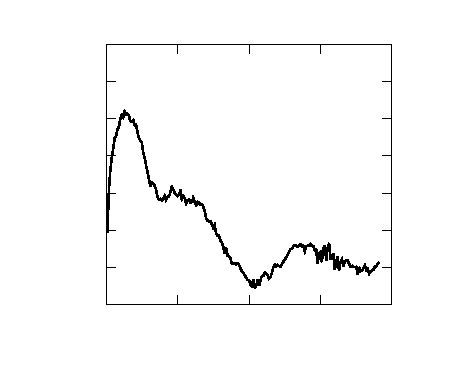
\includegraphics{./figures/parts/02/chapters/01/sections/05/pose_globalplanner_willowgarage}}%
    \gplfronttext
  \end{picture}%
\endgroup

     \vspace{0.75cm}
     \caption{\small WILLOWGARAGE}
   \end{subfigure}
\caption{\small Μέσος όρος σφαλμάτων εκτίμησης στάσης κατά τη διάρκεια του
         χρόνου σε δέκα πειράματα αυτόνομους πλοήγησης με τη χρήση φίλτρου
         σωματιδίων}
\label{fig:02_01_05}
\end{figure}

